\documentclass[12pt]{article}% Your documentclass. I recommend something from the KOMA script class

%------------------------------------------%
%                Packages
%------------------------------------------%
%These are the packages that we will use in our latex document. 

\usepackage{graphicx}
\usepackage{natbib}	%Bibliography package. It handles citations and can easily change formats. This is done at the end of the document
\usepackage[utf8]{inputenx}% For proper input encoding
\usepackage{adjustbox} %Handles resizing of tables, figures, etc. Based off of page and/or line width/height 
% Packages for tables
\usepackage{booktabs}% For Pretty tables
\usepackage{threeparttable}% For Notes below table
\usepackage{rotating}% To Rotate Table
\usepackage{amsmath, amssymb,mathrsfs} %For using math
\usepackage{bm}
\usepackage{caption} 
\usepackage[list=true]{subcaption} %For having multiple figures within the same one. Figure 1, with part (a) and (b)
%\setcounter{lofdepth}{2}
\usepackage{setspace} %Single, Double Space, etc 
\usepackage[paperwidth=8.5in, paperheight=11in,margin=1in]{geometry} %For controlling the dimensions. Very useful for Posters, etc 
\usepackage{chngpage} 
\usepackage{everypage}%For page numbers on rotated pages
\usepackage[capposition=top]{floatrow}
\usepackage{accents}
\usepackage{float}
\usepackage{comment}
\usepackage{morefloats}
\usepackage{placeins}% To Create Float Barriers so the tables will stay in their sections
\usepackage{pdflscape}

\usepackage{siunitx} %This aligns tables by their decimal and handles processing of the numbers within the tables
  \sisetup{
    detect-mode,
    group-digits      = false,
    input-symbols     = {( ) [ ] - +},
    table-align-text-post = false,
    input-signs             = ,
    %parse-numbers=false,
    %scientific-notation = true,
        %round-mode              = places,
        %round-precision         = 2,
        %input-ignore={,},
    %input-decimal-markers={.},
    %group-separator={,},
        } 
\usepackage{grffile}
\usepackage{soul}
\usepackage{color}
\usepackage{caption}
%\captionsetup[figure]{justification=raggedright,singlelinecheck=off}
\sisetup{separate-uncertainty=true}
\usepackage{mathptmx}
\DeclareCaptionLabelFormat{blank}{}

\usepackage[titletoc]{appendix}
\usepackage{multirow}
\usepackage{ragged2e}
\usepackage{titleps,kantlipsum}


%------------------------------------------%
%              Custom Commands
%------------------------------------------%
%These are the custom commands that I use in the latex document

\newcommand\iid{i.i.d.} %Makes iid a command
\newcommand\pN{\mathcal{N}} %Makes the natural numbers a command


\setcounter{MaxMatrixCols}{20}

\newtheorem{theorem}{Theorem}%[section]
\newtheorem{lemma}[theorem]{Lemma}
\newtheorem{proposition}[theorem]{Proposition}
\newtheorem{corollary}[theorem]{Corollary}
\newtheorem{assumption}[theorem]{Assumption}
\newenvironment{proof}{\paragraph{Proof:}}{\hfill$\square$ \\} %This fixes the problem with dynamic tables for some reason

%For Page Numbers while rotated
\newlength{\hfoot}
\newlength{\vfoot}
\AddEverypageHook{\ifdim\textwidth=\linewidth\relax
\else\setlength{\hfoot}{-\topmargin}%
\addtolength{\hfoot}{-\headheight}%
\addtolength{\hfoot}{-\headsep}%
\addtolength{\hfoot}{-.5\linewidth}%
\ifodd\value{page}\setlength{\vfoot}{\oddsidemargin}%
\else\setlength{\vfoot}{\evensidemargin}\fi%
\addtolength{\vfoot}{\textheight}%
\addtolength{\vfoot}{\footskip}%
\raisebox{\hfoot}[0pt][0pt]{\rlap{\hspace{\vfoot}\rotatebox[origin=cB]{90}{\thepage}}}\fi}
%http://tex.stackexchange.com/questions/209685/landscape-mode-and-page-numbering
\newpagestyle{mypage}{%
  \headrule
  \sethead{\shortstack[l]{Section \thesubsection:~\subsectiontitle }}{}{}
  \setfoot{}{\thepage}{}
}
\settitlemarks{section,subsection,subsubsection}

%------------------------------------------%
%      Matter Related to Table Creation
%------------------------------------------%
%This helps with custom automatic tables. It uses latex  functions
%http://www.jwe.cc/2012/03/stata-latex-tables-estout/
%http://repec.org/bocode/e/estout/estout.html

% *****************************************************************
% Estout related things
% *****************************************************************
\let\estinput=\input % define a new input command so that we can still flatten the document

\newcommand{\estwide}[3]{
    \vspace{.75ex}{
      \textsymbols% Note the added command here
      \begin{tabular*}
      {\textwidth}{@{\hskip\tabcolsep\extracolsep\fill}l*{#2}{#3}}
      \toprule
      \estinput{#1}
      \bottomrule
      \addlinespace[.75ex]
      \end{tabular*}
      }
    } 

\newcommand{\estauto}[3]{
    \vspace{.75ex}{
      \textsymbols% Note the added command here
      \begin{tabular}{l*{#2}{#3}}
      \toprule
      \estinput{#1}
      \bottomrule
      \addlinespace[.75ex]
      \end{tabular}
      }
    }

% Allow line breaks with \\ in specialcells
\newcommand{\specialcell}[2][c]{%
    \begin{tabular}[#1]{@{}c@{}}#2\end{tabular}
}
\DeclareUnicodeCharacter{00A0}{ }
% *****************************************************************
% Custom subcaptions
% *****************************************************************
% Note/Source/Text after Tables
% The new approach using threeparttables to generate notes that are the exact width of the table.
\newcommand{\Figtext}[1]{%
  \begin{tablenotes}[para,flushleft]
  \hspace{6pt}
  \hangindent=1.75em
  #1
  \end{tablenotes}
  }
\newcommand{\Fignote}[1]{\Figtext{\emph{Note:~}~#1}}
\newcommand{\Figsource}[1]{\Figtext{\emph{Source:~}~#1}}
\newcommand{\Starnote}{\Figtext{* p $<$ 0.1, ** p $<$ 0.05, *** p $<$ 0.01. Robust standard errors in parentheses.}}% Add significance note with \starnote
% If you are using hyper-ref (recommended), this command must go after all 
% other package inclusions (from the hyperref package documentation).
% The purpose of hyperref is to make the PDF created extensively
% cross-referenced.

\newcommand{\sym}[1]{\rlap{#1}} %Allows for fancy stars in tables that also works in beamer
%\newcommand{\sym}[1]{~} %Allows for fancy stars in tables that also works in beamer

% Create a function that works for the non-linear symbols
\newcommand{\nlsym}[1]{\rlap{\append{}{*}{#1}}} %Allows for fancy stars in tables that also works in beamer
%\newcommand{\nlsym}[1]{~} %Allows for fancy stars in tables that also works in beamer

% Character substitution that prints brackets and the minus symbol in text mode. Thanks to David Carlisle
\def\yyy{%
  \bgroup\uccode`\~\expandafter`\string-%
  \uppercase{\egroup\edef~{\noexpand\text{\llap{\textendash}\relax}}}%
  \mathcode\expandafter`\string-"8000 }

\def\xxxl#1{%
\bgroup\uccode`\~\expandafter`\string#1%
\uppercase{\egroup\edef~{\noexpand\text{\noexpand\llap{\string#1}}}}%
\mathcode\expandafter`\string#1"8000 }

\def\xxxr#1{%
\bgroup\uccode`\~\expandafter`\string#1%
\uppercase{\egroup\edef~{\noexpand\text{\noexpand\rlap{\string#1}}}}%
\mathcode\expandafter`\string#1"8000 }

\def\textsymbols{\xxxl[\xxxr]\xxxl(\xxxr)\yyy}


%Protects against odd minus sign errors within the tables
\catcode`_11
\protected\def \c__siunitx_minus_tl {$-$}
\catcode`_ 8 

%-----------Tables-------------%
% This Section is needed to make the tables work with amsmath. But because of the \( being open and having no match, Sublime Text thinks that everything after it (all text) is in math mode and hence changes the text color. This annoys me so the only ``solution'' is to just place this preamble here. It seems to work still. 
\makeatletter 
\edef\originalbmathcode{%
    \noexpand\mathchardef\noexpand\@tempa\the\mathcode`\(\relax} %\)

\def\resetMathstrut@{%
  \setbox\z@\hbox{%
    \originalbmathcode

    \def\@tempb##1"##2##3{\the\textfont"##3\char"}%
    \expandafter\@tempb\meaning\@tempa \relax
  }%
  \ht\Mathstrutbox@\ht\z@ \dp\Mathstrutbox@\dp\z@
}
\makeatother %./tables.tex:25: LaTeX Error: Bad math environment delimiter. [\)]
\usepackage{xparse}

\ExplSyntaxOn
\DeclareExpandableDocumentCommand{\append}{mmm}
 {
  #1\prg_replicate:nn{#3}{#2}
 }
\ExplSyntaxOff

\doublespacing

%------------------------------------------%
%     Hyper Ref
%------------------------------------------%
\usepackage[colorlinks,linkcolor=black,citecolor=black,urlcolor=black,hyperfootnotes=false]{hyperref} 

%------------------------------------------%
%   Appendix settings
%------------------------------------------%
% Appendix- Table of contents settings
% Make sure table of contents name is correct
\renewcommand{\contentsname}{Appendix table of contents}
% Make sure sections do not get stored in the table of contents
 \addtocontents{toc}{\protect\setcounter{tocdepth}{0}}


%------------------------------------------%
%   Referee Replies
%------------------------------------------%
 \usepackage{csquotes}
 \usepackage{microtype,xparse,tcolorbox}
\newenvironment{reviewer-comment }{}{}
\tcbuselibrary{skins}
\tcolorboxenvironment{reviewer-comment }{enhanced,
	left = 1em, top = 1ex, bottom = 1ex,
}

\newenvironment{in-paper-quote}{}{}
\tcbuselibrary{skins}
\tcolorboxenvironment{in-paper-quote}{enhanced,
	left = 1em, top = 1ex, bottom = 1ex, colupper=black, colback=white,
}
\ExplSyntaxOn
\NewDocumentEnvironment {response} { +m O{black!20} } {
	\IfValueT {#1} {
		\begin{reviewer-comment~}
			\setlength\parindent{2em}
			\noindent
			\ttfamily #1
		\end{reviewer-comment~}
	}
	\par\noindent\ignorespaces
} { \bigskip\par }

\NewDocumentCommand \Reviewer { m } {
	\section*{Reviewer~#1}
}
\ExplSyntaxOff
%\AtBeginDocument{\maketitle\thispagestyle{empty}\noindent}

% You can get probably get rid of these definitions:
\newcommand\meta[1]{$\langle\hbox{#1}\rangle$}
%\newcommand\PaperTitle[1]{``\textit{#1}''}

\begin{document}
   
% Set spacing 
\onehalfspacing



%------------------------------------------%
%     Title Page
%------------------------------------------%

\begin{titlepage}
%\vspace*{.1cm}
\begin{center}
\renewcommand{\thefootnote}{\fnsymbol{footnote}}
%\textbf{PRELIMINARY DRAFT: PLEASE DO NOT DISTRIBUTE}

\textbf{
\noindent\Large
\title
~
Comparative Effects of Recreational and Medical Marijuana Laws On Drug Use Among Adults and Adolescents
}

\vspace{.25cm}
%\vspace{.4cm}

{\large Alex Hollingsworth, Coady Wing, and Ashley C. Bradford\footnote{Hollingsworth: \href{mailto:hollinal@indiana.edu}{hollinal@indiana.edu}. O'Neill School of Public and Environmental Affairs. Indiana University, 1315 E. Tenth Street, Bloomington, IN, 47405 and National Bureau of Economic Research. 
Wing: \href{mailto:cwing@indiana.edu}{cwing@indiana.edu}. O'Neill School of Public and Environmental Affairs. Indiana University, 1315 E. Tenth Street, Bloomington, IN, 47405. 
Bradford: \href{mailto:asbrad@iu.edu}{asbrad@iu.edu}. O'Neill School of Public and Environmental Affairs. Indiana University, 1315 E. Tenth Street, Bloomington, IN, 47405.

We thank Patrick Carlin, Livy Crim, Ted Joyce, Tony LoSasso, Shyam Raman, and participants in the health workshop at Indiana University for their helpful comments.}} \\


\vspace{1cm}
{\large May 2022}\\%\vspace{.25cm}
%First version: October 2018 \\
%\vspace{.25cm}
\end{center}
%\vspace{.5cm}

\begin{abstract}
\begin{singlespace}

Thirty-four states have adopted medical marijuana laws and ten states have adopted recreational marijuana laws. There is little research comparing how these two types of laws affect drug consumption in the general population or in specific age groups. Using a difference in difference strategy, we find that recreational laws increase past-year marijuana use by 25\% among adults and by 10\% among adolescents. In contrast, medical laws increase adult use by only 5\% and have a negligible effect on adolescent use. We also find that recreational marijuana dispensaries are an important driver of the increase in marijuana use for adults 26 and over. Our results suggest that medical laws succeed in mitigating recreational (non-medical) use, that recreational laws produce large increases in marijuana use in the general population, and that underage marijuana use may be an important problem with existing implementations of recreational marijuana laws.

\end{singlespace}
%\end{smallsize}
\end{abstract}

\vspace{3cm}
\begin{singlespace}
{\small
    \noindent\textbf{JEL:} I18, I10, K32 \\
    ~\\
    \noindent\textbf{Keywords:} marijuana use, recreational marijuana, medical marijuana, substance abuse, adolescent drug use
}
\end{singlespace}
%\vspace{.6cm}

\setcounter{footnote}{0}
\end{titlepage}
     
%------------------------------------------%
%     Introduction
%------------------------------------------%

\onehalfspacing 

\section{Introduction} 
\label{sec:Introduction}

State governments are experimenting with policies that create legal marketplaces for marijuana. Thirty-four states have medical marijuana laws, which legalize marijuana consumption for people with a qualifying medical condition \citep{ProCon2018b}. More recently, ten states have adopted recreational marijuana laws that legalize marijuana consumption for adults without any qualifying health rationale \citep{ProCon2018}. These changes are controversial. The federal government and many states continue to have prohibition policies that make it illegal to sell and possess marijuana. 
The move to legalize marijuana use expands personal liberty in ways that seem consistent with core ideas about American government. But creating and managing regulated markets for psychoactive substances is complicated and may have unintended consequences. Even if recreational drug use is viewed as a matter of personal liberty, there may be a role for government in supplying information about the quality of drugs on the market and the possible side-effects of drug use. In addition, legalizing marijuana may increase drug use in the general population, which could produce negative externalities. Underage marijuana use is another concern. Recreational laws prohibit children and adolescents from buying and consuming marijuana, but these age restrictions may be hard to enforce in practice. Similarly, medical marijuana laws are designed to allow marijuana use among people with qualifying health conditions. They are not supposed to facilitate recreational marijuana use. However, it is unclear how well medical marijuana laws are able to exclude recreational users from medical markets.
In this paper, we bring data to bear on three questions about recent marijuana policy changes. First, how much do recreational laws alter the prevalence of marijuana use in the general population of U.S. adults? Second, do marijuana laws control underage marijuana use? Third, are medical laws \emph{de facto} recreational laws? That is, are people without qualifying health conditions just as able to obtain marijuana from medical markets as they would be from recreational markets? Our main analysis is based on data from the National Survey of Drug Use and Health Small Area Estimates (NSDUH SAE), and we use a generalized difference in difference (DID) design that exploits multiple policy changes. We find that recreational laws increase past-year marijuana use by about 15 percent among adults ages 18 to 25, and about 25 percent among adults over age 25. Access to dispensaries, physical locations where medical or recreational marijuana can be bought, are a key driver of the increases in use for those over the age of 25. Furthermore, our results suggest that that recreational laws are ineffective at controlling underage marijuana use. Specifically, adopting a recreational law increases marijuana use among adolescents ages 12 to 17 by about 10 percent. Our findings indicate that legalization increases marijuana use more for older age groups than for younger age groups. This is consistent with predictions by \citet{Jacobi2016}, who show using Australian data that younger age groups have greater pre-legalization access to marijuana and that access is an important predictor for post-legalization use. 

Across all age groups, the effects of recreational laws are quantitatively large, statistically significant, and are not sensitive to an extensive set of robustness checks and changes in model specification. In contrast, medical laws have much smaller effects. In most age groups, the effect of recreational laws on marijuana use  is three to four times larger than the effect of medical laws. One interpretation is that recreational laws increase marijuana use in the general population, but medical laws mainly affect marijuana consumption in a smaller sub-population of people with qualifying health conditions. We also find some evidence that medical marijuana laws may lead to small reductions in alcohol and tobacco use, and that recreational laws may increase cocaine use. However, these results are less stable and are sensitive to specification choice. 

We first present results from event-study specifications.  
For the measures of adult use, we find no evidence that adopting states have differential time trends in substance use prior to  recreational adoption. 
The event study point estimates of how adolescent marijuana use changes before and after recreational adoption are smaller and somewhat noisier, but still strongly suggest that legalization increased adolescent use. 
Our main results come from two-way fixed effect models. 
We use a decomposition technique to clarify the key sources of variation underlying the results \citep{Goodman-Bacon2018}, estimate event study models to test for differential pre-trends, and implement a series of supplementary analyses that examine common trend assumptions, compositional change, alternative model specifications (covariates, transformations of the outcome variable, and use of weights),  alternative approaches to statistical inference, alternative sample inclusion criteria, and alternative ways of coding policy changes. The core results are very stable across these tests.  The Goodman-Bacon decomposition demonstrates that the early adopting states are not driving our findings. 

We also assess the extent to which our results are affected by features of the dataset we use in our analysis. The NSDUH SAE is a state-year level data that is released in overlapping two-year waves. We ensure that this structure is not driving or otherwise biasing our estimates away from zero by considering specifications with alternative treatment timing, by estimating specifications using every other year of data (so there is no overlap across waves), and by considering alternative constructions of p-values based on randomization inference procedures.  Our estimated treatment effects and estimates of statistical significance are consistent across all of these checks. 

Our work relies heavily on survey based estimates of drug use from multiple waves of the NSDUH. One concern is that efforts to legalize marijuana may affect the extent to which NSDUH respondents are willing to give truthful and accurate answers to questions about drug use. We think the NSDUH is the best available data source for measuring marijuana use in representative samples of adults and adolescents in the U.S. and we found no evidence that there has been a change in measurement differences between the NSDUH and alternative school based surveys like the Youth Risk Behavior Survey (YRBS). However, to supplement our analysis of the NSDUH data, we also study the effects of recreational and medical marijuana laws using two non-survey data sources. First, using data from workplace drug tests, we find that recreational marijuana laws increase the the fraction of workplace drug tests that are positive for marijuana by about 30 percent. Second, using data from the FBI Uniform Crime Reports (UCR) we find that, recreational marijuana laws reduce adult arrests for marijuana possession by about 50 percent and increase juvenile arrests for marijuana possession by about 60 percent.  The non-survey results are interesting in their own right, but we view them as supporting evidence for our main result, which is that recreational marijuana laws generate substantial increases in the prevalence of marijuana use among adults and adolescents. 

Our study is the first quasi-experimental analysis of the causal effects of recreational laws on marijuana use in the general population of adults and adolescents in the United States. Most prior work examining the effects of recreational marijuana laws on marijuana use focuses on the narrower sub-population of current students. We are also the first to compare the differential effect that dispensaries of both medical and recreational marijuana may have on marijuana use in the United States.

The results of our analysis may be useful for developing new state marijuana policies and for fine tuning existing policies. In particular, our analysis of underage marijuana use is salient to recent debates as we find evidence that recreational marijuana adoption increases adolescent marijuana use. The medical community argues that marijuana use is likely most harmful for children and adolescents, who still have developing brains and are at a greater risk of impaired development from substance use \citep{AmericanAcademyofPediatrics2015}. While most advocates seem to accept this view, there is considerable public debate about whether legalization will increase \citep{MacleanMJUse2021,cerda2020association, Dudek2019}, decrease  \citep{Blumenfeld2019, Sepeda-Miller2019, Anderson2019}, or have no effect on adolescent marijuana use \citep{Anderson2015,Sarvet2018}. Our results cast doubt on the view that recreational marijuana laws will reduce adolescent marijuana use.

The results also contribute to research on the public health effects of marijuana policy. For example, \citet{Anderson2013} find that medical laws reduce traffic fatalities by 9\%; \citet{Bachhuber2014} and \citet{Powell2018} find that medical laws reduce opioid mortality by 20\%; and \citet{Chan2019} find that recreational laws reduce opioid mortality by 7\%. The most plausible interpretation of these results is that these laws lead to substitution between marijuana and other drugs. The results of our study help put these ``reduced form'' results in perspective by shedding light on the first stage effect of legalization on the use of marijuana. They also suggest that the larger increases in marijuana use produced by recreational laws may have larger effects on social outcomes than medical laws.

Our paper proceeds as follows. Section~\ref{sec:background} provides  background on marijuana policy and prior research.  Sections~\ref{sec:Data} and~\ref{sec:Methods} describe our data, research design, and econometric methods. Section~\ref{sec:Results} reports the results, sensitivity of our p-values to a randomization inference procedure, and a balance table comparing non-drug use outcomes between recreational marijuana states and other states. Section~\ref{sec:Conclusion} concludes. The Appendix reports policy adoption dates used in our analysis and the Online Appendix contains robustness checks, supplementary analyses, and other supporting information.

%------------------------------------------%
%     Background
%------------------------------------------%

\section{Background} 
\label{sec:background}

In the United States, marijuana has been illegal under federal law since 1970 when Congress passed the Controlled Substances Act (CSA). Under the CSA, marijuana is assigned to \textit{Schedule I}, which is reserved for drugs with “no currently accepted medical use and a high potential for abuse” \citep{DEA2019}. Despite the federal prohibition, states started to introduce medical marijuana laws in the 1990s. In 1996, California adopted the first medical law, which allowed adult California residents to use marijuana for medical purposes provided that the use is recommended by a licensed physician \citep{Reinarman2011}. Since then, thirty-three states and the District of Colombia have adopted medical laws that allow adults to use marijuana if they have specified health conditions \citep{ProCon2018b}.\footnote{The details of medical marijuana laws vary across states. Some states allow caregivers to cultivate and distribute marijuana; others have mandatory registration requirements. Some states cap the quantity of marijuana that person can legally possess, allow home cultivation, and allow dispensaries. In addition, the list of qualifying conditions that a patient must present to a physician in order to receive a medical marijuana recommendation varies across states.} In 2012, Colorado and Washington became the first states to adopt recreational marijuana laws, which permit adults to use marijuana without any health related justification. Since then, eight more states and the District of Columbia have adopted recreational laws \citep{ProCon2018}. To date, each of the recreational marijuana states had already adopted medical marijuana laws when the recreational laws were passed.

All recreational marijuana states prohibit the sale, purchase, and consumption of marijuana among people under age 21. However, other details of the laws vary across states. Colorado and Washington require marijuana to be tested before it is sold \citep{ThePolicySurveillanceProgram2015}. Home cultivation is allowed in all recreational states except Washington and Illinois. The states have different limits on the maximum quantity of marijuana one can legally possess, different legal limits for driving under the influence of marijuana, different licensing standards for cultivation facilities and retail outlets, and different administrative fees and taxes on sale of marijuana \citep{ThePolicySurveillanceProgram2015}. None of the recreational marijuana states restricts the potency of marijuana. Some states levy an excise tax on marijuana at a flat rate per ounce. Other states collect a percentage of the average retail price, which may act as a tax on the potency of the cannabis because average prices are closely related to potency \citep{Hanson2015}. The level of the tax varies across states, and marijuana tax revenue is often earmarked for enforcement, educational, and prevention campaigns \citep{Hanson2015, Hansen2017}.\footnote{Alaska collects \$50 tax per ounce from producers. California collects a 15\% sales tax from consumers and levies a cultivation tax on producers at a rate of \$9.25 per ounce of flowers and \$2.75 per ounce of leaves. Colorado recreational users pay a 15\% sales tax and a 15\% marijuana excise tax. In Massachusetts, the excise tax is 10.75\% and it does not levy a sales tax. Nevada also imposes a sales tax of 10\%, and an excise tax of 15\%. Oregon collects a 17\% sales tax but does not collect a marijuana specific excise tax. Finally, Washington collects a sales tax of 37\% \citep{TaxFoundation2018}.}


\subsection{Medical marijuana laws and marijuana use}\label{sec:mml_related_research}

A number of previous studies have explored the relationship between medical marijuana adoption and marijuana use. 
A series of papers provide evidence that medical marijuana adoption is associated with an increase in marijuana use for adults \citep{Cerda2012, Martins2016, WEN201564}. 
\citet{Pacula2015} and \citet{Hasin2017} find that the increase in adult use is driven by medical marijuana laws that allow for dispensaries. 
Other work has found that less restrictive medical marijuana laws are associated with increased consumption  \citep{Anderson2013,Smart2015,Sabia2017,Powell2018}. 
In line with the literature, in our analyses we distinguish between medical and recreational marijuana laws that allow for dispensary access and those that do not in order to control for the differential access that dispensaries could offer. 


Several studies report that medical marijuana laws reduce prescription drug use among publicly and privately insured patients and also reduce opioid overdose mortality \citep{Bachhuber2014,Bradford2018, Ozluk2017,Powell2018}.
\citet{Anderson2013} found medical laws decrease alcohol consumption, and \citet{WEN201564} found that they increased binge drinking for adults and had no effect on alcohol use for adolescents.
\citet{Choi2019} found that medical laws reduce cigarette consumption.
There is a small literature concerned with the effects of medical marijuana laws on non-substance use outcomes, including crime \citep{Morris2014,Gavrilova2017}, body weight \citep{Sabia2017}, and wages \citep{Sabia2018}. 
These studies provide indirect evidence that medical marijuana adoption increases marijuana use under the assumption that the reduced form effects in these studies are driven by an underlying increase in marijuana use. 

A key concern is that marijuana legalization may increase marijuana use among children and adolescents \citep{Anderson2014,Hall2015a,Hall2016,NationalAcademiesofSciencesEngineering2017,Salomonsen-Sautel2012,Thurstone2011,Volkow2014}. 
Previous research provides little evidence that medical marijuana adoption increases youth marijuana use.\footnote{\cite{Hasin2015} and \cite{Wall2011} find that adolescents living in  medical states had higher levels of marijuana use, but when \cite{Harper2012} extended that analysis to account for unmeasured heterogeneity and measurement error, they found no impact on past-month adolescent use. Similarly, \cite{Stolzenberg2016} found that the passage of medical marijuana laws was associated with an increase in adolescent marijuana use, but \cite{Wall2016} replicated the study and concluded that the previous study had not adequately controlled for the fact that medical states tend to have higher rates of marijuana use before medical laws were enacted.}
Many studies find no relationship between medical adoption and youth use \citep{Anderson2019, Anderson2015, Choo2014, Harper2012, Lynne-Landsman2013, Wall2016} and some find a reduction in use \citep{Johnson2017, Keyes2016}. 
Recent work has also explored how medical marijuana adoption has changed the perceived riskiness of marijuana use, but that this change in perception was not accompanied by a change in use among adolescents  \citep{Wen2018a,Sarvet2018}.


\subsection{Recreational marijuana laws and marijuana use}\label{sec:rml_related_research}

Because recreational laws are a recent phenomenon, there is not much previous work examining the ways they affect the use of marijuana and other drugs.\footnote{We focus on the American case. For studies of marijuana regulation in the Netherlands, see \citep{Korf1995, Monshouwer2004, MacCoun2001,MacCoun2010}} 
\citet{Wen2018} find that both medical and recreational laws reduce opioid prescribing rates in the Medicaid program;  \citet{Hollingsworth2019} find that Colorado’s recreational marijuana law reduced sales of alcohol products that have low cost per unit of alcohol; and \citet{Miller2018} find that alcohol and tobacco sales decrease following recreational legalization in Washington. 
As with the medical marijuana literature, these studies provide indirect evidence that recreational marijuana laws may increase marijuana use under the assumption that the effects on other outcomes are driven by a substitution towards marijuana use following the liberalization. 

Using Australian data, \citet{Jacobi2016} find that people who have more access to marijuana prior to legalization are less likely to increase marijuana use following legalization. 
They also show that pre-legalization access to marijuana is correlated with age, with younger groups reporting greater access. 
Due to these differences in pre-reform access, \citet{Jacobi2016} predict that if Australia legalized marijuana younger people would see a smaller change in marijuana use than older people. Assuming that -- under prohibition -- access to marijuana is correlated with age in the United States the way it is in Australia, a testable prediction is that the effects of recreational marijuana laws on marijuana use will vary by age and will have a smaller effect on younger people. 



\citet{Dills2017} and \citet{Cerda2017} study marijuana regulations in the U.S. using data on high school students in the Monitoring The Future (MTF) study. \cite{Dills2017} find no evidence that liberalization affects high school drug use or related behaviors. \cite{Cerda2017} use a version of a two group - two period DID based on logistic regressions. They find that Washington’s recreational laws increased marijuana use among the 8th grade and 10th grade students. They do not find evidence that Colorado’s recreational law affected drug use. 
\citet{Dilley2019} use a school-based survey in Washington to show that the average prevalence of 8th and 10th grade marijuana use declined following legalization. The survey they use is only conducted in Washington so they cannot compare these reported declines in marijuana use to a control group of students in a state that did not legalize marijuana. 
\cite{Kerr2017} studied Oregon's recreational law using data on university students. They estimated a mixed-effects logistic regression model, which suggested that Oregon’s recreational law increased marijuana use among students at one university in Oregon, but only among students who also reported being heavy alcohol consumers. \citet{Anderson2019} examine the relationship between medical and recreational adoption and self-reported past-month marijuana use among high school students using pooled data from the national and state Youth Risk Behavior Surveillance System (YRBSS). They find that recreational marijuana laws reduced the odds of marijuana use by 9\% among high school students. The closest study to ours is a recent paper by  \cite{cerda2020association}, which examines the association between recreational marijuana laws and measures of marijuana use and cannabis use disorder using data from the NSDUH. \cite{cerda2020association} estimate a mixed effects logistic regression that incorporates a state level random effect, a cubic spline in the survey year to model a national time trend, and a vector of time varying covariates. Using this model, they report slight increases in adolescent use, no increase in young adult use, and increases in older adult use. They also report an association between recreational legalization and cannabis use disorder in older adults. Our model differs from \cite{cerda2020association} by accounting for key sources of bias using a quasi-experimental difference-in-differences framework. We use state fixed effects to account for time-invariant unobservables, region-by-year fixed effects to account for region specific changes that vary across time, and include a number of robustness checks that ensure our results are not driven by endogenous policy selection. \citet{MacleanMJUse2021} also use the NSDUH SAE to examine how past year marijuana use increases following legalization. They show that recreational adoption increases use for those 12 and up by 28.8\%, but do not separately examine effects by age-group or for other measures of marijuana use.  


%------------------------------------------%
%     Data
%------------------------------------------%   

\section{Data} 
\label{sec:Data}

\subsection{National Survey of Drug Use and Health}
\label{sec:data_nsduh}

We use data from the National Survey of Drug Use and Health (NSDUH), which is an annual representative sample of the civilian, non-institutionalized population aged 12 and older living in the United States. Geographical identifiers are not available in the public use NSDUH. However, the NSDUH Small Area Estimation (SAE) files provide state-level prevalence estimates based on data from two adjacent years of NSDUH microdata (SAMHSA, 2015; Wright, 2003).\footnote{The NSDUH SAE have be used in previous research by \cite{Choi2019,Friedman2015}. The NSDUH SAE data are reported in two-year waves. We ensure that this overlapping structure is not driving our findings by considering specifications with alternative treatment timing, by estimating specifications using every other year of data to ensure no overlapping data, and by considering alternative constructions of p-values based upon randomization inference procedures. These checks are outlined in more detail in the Online Appendix.} 
%

The main substance use outcomes we study are NSDUH SAE state level age-specific drug use prevalence estimates from 2001-2002 to 2016-2017. We study five age groups reported in our data:  12 and up, 18 and up, 26 and up, 12-17,  and 18-25. For each age group we examine prevalence of: (i) any marijuana use in the previous year, (ii) any marijuana use in the previous month, (iii) first time marijuana use in the past two-years, (iv), any alcohol use in the previous month, (v) any tobacco use in the previous month, (vi) any cocaine use in the previous year. 

%------------------------------------------%
%                Table 1
%------------------------------------------%
% Summary statistics
    \begin{table}[ht]\centering
            \begin{adjustbox}{width=\textwidth}
            \centering
              \begin{threeparttable}
                \caption{Substance use percent [0-100] by substance and by age group, 2002/2003-2016/2017}
                \estauto{../output/tables/summary_statistics.tex}{6}{S[table-format=1.2,table-column-width=20mm]}
                \label{tab:summary_statistics}
               % \Figtext{Some basic text about the table.}
                \Fignote{N=765 (state-years). Mean reported, standard deviation in parentheses. First use is the percentage of those who tried marijuana for the first time in the past two years out of those who had never tried the drug before.}                %\Figsource{We good the data from here.}
              % \Starnote
              \end{threeparttable}
             \end{adjustbox}
        \end{table}

Table~\ref{tab:summary_statistics} reports summary statistics of each substance use measure for each age group across the states and years in our study period. The table shows that in the average state-year in our sample, the prevalence of past-year marijuana use was roughly 14\% for adolescents, 31\% for 18 to 25 year olds, and 9\% for those aged 26 and over. Rates of past-month marijuana use are roughly half the past-year use across all age-groups. 

An alternative source of survey data on adolescent drug use is the Youth Risk Behavior Survey (YRBS). However, there are several reasons for which we determined that the NSDUH would be the superior option in this case. First, the NSDUH samples from both adults and adolescents, while the YRBS only includes adolescents. In addition, the YRBS is a school-based survey. This means that any adolescents that are not attending school during survey collection are not included. The YRBS also does not include data from all states in every year, whereas the NSDUH does. Finally, the YRBS is a pen-and-pencil survey. The NSDUH, on the other hand, is taken using Audio Computer Assisted Self Interview (ACASI), which means that the respondent wears headphones, listens to recorded questions, and enters their own responses on a laptop computer. This is meaningful in this context, as there is a body of evidence indicating that there is higher rates of reporting for risky behaviors when surveys are given in ACASI format rather than pen-and-pencil. A full discussion comparing the pros and cons of using the YRBS versus the NSDUH can be found in the online appendix. 


Despite these advantages, the NSDUH measures we use in our analysis are still based on self-reported information about sensitive topics. The survey data may include reporting errors that arise if respondents are embarrassed, ashamed, or afraid to answer questions about illegal or stigmatized activity. Since the difference-in-difference research design that we use in the paper is based on changes in state recreational marijuana laws, the primary concern for identification is that the frequency of survey reporting errors has changed over time because of the policy changes. For example, if legalizing marijuana makes people more willing to admit to using marijuana, then difference-in-difference estimates of the effects of the laws on marijuana use may be confounded by an increase in willingness to report.  This issue may be particularly salient for adolescents. In Figure~\ref{fig:nsduh-v-yrbs}, we present a supplementary analysis that compares national time series data from the NSDUH and the YRBS to assess the likelihood that the recent wave of marijuana deregulations has altered the way that adolescents respond to survey questions about marijuana use. The reporting gap between the NSDUH and YRBSS does not change as more states legalize recreational marijuana suggesting this is not an issue.


\subsection{Marijuana Laws }\label{sec:data_laws}

We collected information on recreational and medical marijuana laws from the \cite{NationalAllianceforModelStateDrugLaws2017a,NationalAllianceforModelStateDrugLaws2017}, ProCon.org, \cite{Powell2018}, and the language of individual state laws. In our main analysis, we coded policy adoption as the first year in which it was legal under state law for residents to possess and consume marijuana within the limitations of each individual state law. Some of our analysis also examines the effects of dispensaries. Although dispensaries are typically envisioned by the same law that legalizes possession and consumption, dispensaries typically do not actually open until one or more years after possession and consumption become legal. We collected data on dispensary opening dates in each state, for both medical and recreational dispensaries, by searching state and local newspaper articles for mentions of the first recreational or marijuana dispensary in the state and confirming using multiple sources. Citations for the source of our information on  the date of initial passage, the date when legal protections were provided, and the date when the first dispensary opened are available in an online replication package.\footnote{\url{https://github.com/hollina/recreational-marijuana-legalization-and-use}.}



Table~\ref{tab:adoption_table} reports the adoption year for each medical and recreational marijuana law, and the dispensary opening dates that we use in our analysis.  The table also reports the two-year NSDUH wave that we consider to be treated in parentheses after each year. We use a conservative timing assignment in our preferred analysis. Specifically, we consider a two-year NSDUH period to be \textit{treated} if the policy was in effect in both years of the wave. For example, if a recreational marijuana law was implemented in a given state in 1999, we code that state as untreated in the NSDUH 1998-1999 wave and treated in the NSDUH 1999-2000 wave. In essence, we code some partially treated waves of data as untreated. This method is conservative in the sense that it likely attenuates our estimates of the effects of the law and makes it less likely that we will find evidence that the policy changes affected levels of drug use. 



In addition to the conservative coding scheme we use in the main analysis, we also consider two alternative strategies as robustness checks. First, we repeat our main analysis using a sample of data in which we drop every other year of data to avoid any overlap across panel years. This tests if the overlapping structure of the SAE data is driving our results. Second, we consider a more aggressive definition of treatment adoption, which codes a two-year NSDUH wave as treated if the policy was implemented in either of the years.\footnote{This aggressive definition approach is similar to work by \citet{Friedman2015} who used the NSDUH SAE to study the effects of e-cigarette bans on adolescent smoking.} These results are presented in the results and appendix sections of the paper.

\subsection{Workplace Testing Data and Marijuana Arrest Data}

The central questions in our study revolve around the effects of state medical and recreational marijuana regulation on the prevalence of marijuana use among adults and adolescents. As such, we primarily measure the prevalence of marijuana use using survey data. However, a possible alternative interpretation of our results on marijuana use is that they reflect changes in the survey measurement patterns rather then genuine increases in marijuana use in the population. To help probe the plausibility of this alternative interpretation, we also examine broader effects of marijuana regulations using non-survey data sources that should not be subject to the same concerns about willingness to self-report. These analyses are also substantively interesting because they provide insight into the way that marijuana laws are affecting outcomes in workplace and criminal justice settings. 

To study the prevalence of marijuana use using non-survey data, we examine data from Quest Diagnostics, a commercial lab that conducts workplace drug tests on behalf of employers \citep{questdiagnostics}. The outcome variable we analyze is simply the fraction of workplace drug tests conducted by Quest Diagnostics that positive for tetrahydrocannabinol (THC)---the primary psychoactive component of marijuana---in each state $\times$ year cell.
We use the data to study the effects of state marijuana laws on the positive test rates using the same regressions used for our survey based measures of the prevalence of marijuana use. Additionally, state marijuana laws  have important implications for the criminal justice system. Legalizing the production, sale, and consumption of marijuana under certain conditions reduces the number of people who are breaking the law and thus may reduce the number of people arrested for drug related crimes. However, the laws may increase marijuana use overall and some of the increased marijuana use may still be illegal (for example, underage marijuana use.) The number of marijuana arrests may also depend on the level of law enforcement effort devoted to marijuana related crimes, and it is possible that medical and recreational marijuana laws affect enforcement effort allocation as well. To study these issues, we work with the concatenated version of the FBI Uniform Crime Report arrest files provided by \citet{kaplan2020}. For a full discussion of the Quest Diagnostics and UCR Data, see the Online Appendix. 

\subsection{Covariates}\label{sec:data_covariates}

Our preferred models adjust for a set of state level time-varying covariates. Primarily, we control for macroeconomic indicators and demographic characteristics that have been linked to adverse substance use outcomes by \cite{Hollingsworth2017} and \cite{Ruhm2018}. We obtained annual data on state median income and unemployment rates from the Bureau of Labor Statistics. We use annual data from the Surveillance, Epidemiology, and End Results project to measure state population size and composition with respect to race, sex, ethnicity, and age. Data on state-level violent and property crime rates were obtained from the Uniform Crime Reports. Appendix Table~\ref{tab:summary_statistics_other} reports summary statistics on the covariates.
    
%------------------------------------------%
%               Methods
%------------------------------------------%
\section{Econometric Methods} 
\label{sec:Methods}

Our study is built around a generalized (staggered adoption) DID design that exploits multiple marijuana policy changes to estimate the effects of both medical and recreational marijuana laws. Recent work by \cite{Goodman-Bacon2018} emphasizes that conventional two-way fixed effects regressions can be misleading in these settings. To allay these concerns, we use a decomposition technique developed by \cite{Goodman-Bacon2018} to clarify the way the effect estimates are linked to specific policy changes and we present results from event study regressions that trace out drug use in the years surrounding policy changes. Our main analysis is focused on outcome variables that measure the prevalence of marijuana use in specific age groups, as measured by self-reported responses in multiple waves of the NSDUH. However, we also conduct some additional analysis of two non-survey data sources using the same basic econometric strategy. That is, we estimate the effects of state marijuana laws workplace marijuana test positivity rates using data from Quest Diagnostics. And we estimate the effects of marijuana laws on the juvenile and adult marijuana related arrests using arrest data from the FBI UCR database.

\subsection{Difference in Differences}

In the classical two group-two period DID, outcomes in treatment and control groups are measured before and after a change in treatment status in the treated group. For groups $a$ and $b$, the classical DID estimator is $\beta_{ab}^a = (P_a^{Post(t_a,t')} - P_a^{Pre(t'',t_a )}) - (P_b^{Post(t_a,t')} - P_b^{Pre(t'',t_a )})$, where $t_a$ is the treatment adoption date in group $a$, $P_j^{Post(t_a,t')}$ is the average outcome in group $j$ in a post period that runs from $t_a$ to an end date $t'$, and $P_j^{Pre(t'',t_a)}$  is the average outcome in group $j$ in a pre-period running from start date $t''$ to some time before $t_a$. Under the assumption that the two groups would have followed a common trend in the absence of treatment and treatment timing is strictly exogenous of the outcome variable, the probability limit of  $\beta_{ab}^a = ATT_a^{Post(t_a,t' )}$, which is the average treatment effect on the treated for group $a$.

The generalized DID design we use in this paper involves changes in state laws that occur in several states at different times. In our main analysis, we employ two-way fixed effects regressions to combine the variation from each of these policy changes. The idea is to use the statistical model to combine variation from several underlying 2x2 DID designs. A basic version of the analysis is a state-by-year level regression of drug use prevalence (or workplace test positivity, or marijuana arrests) on state and year fixed effects and a recreational marijuana law indicator,
%
\vspace{-.25cm}
\begin{align*}
P_{st} = \beta^{DID} R_{st}+ \theta_s + \delta_t + \epsilon_{st}.
\end{align*}

With two groups and two periods $\beta^{DID} = \beta_{a,b}^a$ and both methods identify $ATT_a^{Post(t_a,t' )}$ . While the fixed effects specification remains feasible with $S>2$ groups and $T>2$ periods, the connection between $\beta^{DID}$ and the underlying design is obscured, and it is not always clear what causal parameter $\beta^{DID}$ identifies. It turns out that $\beta^{DID}$ is a consistent estimator of the causal effect of the regulation if treatment effects are constant across both states and years and the identifying assumptions hold.\footnote{\cite{Wooldridge2005} shows that, even if treatment effects are heterogeneous, $\beta^{DID}$ is consistent for the overall average treatment effect if unit specific treatment effects are independent of the demeaned treatment variable.} \cite{Goodman-Bacon2018} shows that when treatment effects are heterogeneous and potentially correlated with changes in treatment exposure, $\beta^{DID}$ can be decomposed into a weighted average of pairwise classical DIDs. The decomposition is a useful way to understand the sources of variation driving our study. 

Over our study period, there are seven states that adopt recreational marijuana laws and forty-four states that do not adopt recreational marijuana laws.\footnote{Recreational laws were adopted in 2012 (Colorado and Washington), 2015 (Alaska, Oregon, and Washington, DC), and 2016 (California and Massachusetts). Maine, Michigan, Nevada, and Vermont adopted recreational marijuana laws in 2017 and 2018. These changes occurred after the period covered by the NSDUH SAE data and so these states are untreated throughout our study.}

The seven states that adopt recreational marijuana laws make their changes at three different points in calendar time. To make this clear, we group the states into timing groups. Specifically, we use  $k(s)\in\{E,M,L,U\}$ to index the early adopter, middle adopter, late adopter, and untreated groups of states, and we let $t_{k(s)}$  be the adoption year in group $k$.\footnote{This means $t_E=2012$, $t_M=2015$, $t_L=2016$, and $t_U=\infty$. As a result, $R_{st}=1(t\geq t_k(s)$ ) is a indicator set to 1 if a recreational marijuana law was in force in state $s$ in period $t$.}

With three timing groups and one untreated group, there are nine pairwise DIDs in our study. There are three DIDs that compare a treated timing group with the untreated comparisons group: $\beta_{E,U}^E,\beta_{M,U}^M$,and $\beta_{L,U}^L$. Then there are two DIDs for each of the three pairwise comparisons of timing groups: one in which the earlier group serves as the treatment group, and one in which the later group serves as the treated unit and the (already treated) earlier adopting group acts as a control. For instance, to construct $\beta_{E,M}^E$, the early timing group is the treatment group, the middle timing group is the control group, the post period runs from $t_E$ to $t_M$, and the pre-period runs from 2001 to $t_{E-1}$. In contrast, $\beta_{E,M}^M $ is a DID where the early timing group is the control, the post period runs from $t_M$ to 2016, and the pre-period runs from $t_E$  to $t_M$. The DID decomposition shows that,
%
\vspace{-.25cm}
\begin{align*}
\beta^{DID}= &s_{E,U}^E \beta_{E,U}^E + s_{M,U}^M \beta_{M,U}^M + s_{L,U}^L \beta_{L,U}^L \\
+&s_{E,M}^E \beta_{E,M}^E + s_{E,M}^M\beta_{E,M}^M  \\
+&s_{E,L}^E \beta_{E,L}^E + s_{E,L}^L\beta_{E,L}^L  \\
+&s_{M,L}^M \beta_{M,L}^M + s_{M,L}^L\beta_{M,L}^L. 
\end{align*}


In the formula, $s_{k,l}^k$ is the weight associated with the pairwise comparison of groups $k$ and $l$ when group $k$ serves as the treatment group. The weights are determined by the fraction of the sample in each timing group, and the proportion of the time that each timing group is treated.\footnote{Let $n_k$ be the share of the sample that belongs to group $k$. $n_{kl} = \frac{n_k}{(n_k +n_l)} $is the relative size of group $k$ in the $kl$ pair.Let $\bar{R_k}$ be the proportion of periods that timing group $k$ is exposed to treatment. After removing state and year fixed effects, the treatment exposure variable has variance $V(\tilde{D_{st}}) $. The weights  are $s_{kU}^k=\frac{1}{V(\tilde{R_{st}})}[(n_k + n_U)^2 n_{ku}(1-n_{ku})\bar{R_k}(1-\bar{R_k}))] $, $s_{kl}^k=\frac{1}{V(\tilde{R_{st}})}((n_k + n_l) (1-\bar{R_l})^2n_{kl}(1-n_{kl})\frac{\bar{R_k}-\bar{R_l}}{1-\bar{R_l}} \frac{1-\bar{R_k}}{1-\bar{R_l}})$, and $s_{kl}^l=\frac{1}{V(\tilde{R_{st}})}((n_k + n_l)\bar{R_l})^2 n_{kl}(1 - n_{kl})\frac{\bar{R_l}}{\bar{R_k}} \frac{\bar{R_k}- \bar{R_l}}{\bar{R_k}})$.}


Timing groups that represent a large share of the sample get more weight. And timing groups that adopt treatment closer to the middle of the study window get more weight than groups that adopt treatment closer to the start or the end of the study. By computing the weights that apply to our data, we can quantify the relative importance of the specific state policy changes for our study and assess how much treatment effect heterogeneity underlies our pooled fixed effect estimates. In addition, \cite{Goodman-Bacon2018} points out that policy variation that comes from comparisons of a later timing group with an already treated earlier timing group may be at risk of failing the common trends assumption if the effect of the policy is time varying. By computing the weights, we can determine how much emphasis our fixed effects model places on these problematic late vs early comparisons. In this sense, the decomposition weights represent a diagnostic analysis that sheds light on the validity of the two-way fixed effect model. In turn, the two-way fixed effects model should improve statistical efficiency by pooling information from multiple quasi-experiments, providing a more interpretable and parsimonious summary of the effect of the regulatory changes on measures of drug use.

\subsection{Two Way Fixed Effects}
\label{sec:research_design_twoway_fe}

With the decomposition as background, our preferred specification estimates the effects of both recreational and medical laws using an expanded version of a two-way fixed effect regression. The main specification is:

\begin{align}
P_{st}=\beta_1 R_{st}+\beta_2 M_{st}+\beta_3 MD_{st}+x_{st} \alpha+\theta_s+\delta_{r(s)t}+\epsilon_{st}. \label{eq:two_way_fe}
\end{align}

In our main analysis, $P_{st}$ is the log prevalence of a measure of drug use in state $s$ in period $t$ as measured in the NSDUH SAE; however, we also fit some models where the dependent variable is the log positivity rate for the workplace drug testing data, and the number of juvenile and adult arrests for marijuana possession and sales.\footnote{In the analysis of marijuana related arrests, we use fixed effects poisson models rather than linear models. These models maintain a non-negativity constraint and fit the data better than the linear model. However, the results are robust to a linear specification.} $R_{st}$ and $M_{st}$ are dummy variables indicating whether the state had a recreational or medical marijuana law during period $t$. $MD_{st}$ is a dummy variable set to 1 if the state’s medical marijuana law allows dispensaries in year $t$.\footnote{When a state has no medical marijuana law in place then  $M_{st}=MD_{st}=0.$ When a state has a non-dispensary medical marijuana law then $M_{st}=1$ and $MD_{st}=0$. When a state has a dispensary medical marijuana law then $M_{st}=MD_{st}=1$.} $x_{st}$ is a vector of time varying covariates.\footnote{The covariate vector consists of the unemployment rate, median income, \% white, and \% male.} We use $r(s)=(Northeast,Midwest,South,West)$ to index the four census regions so that $\delta_{r(s)t}$ is a region-by-year period fixed effect, which is inclusive of year fixed-effects. $\theta_s$ is a state fixed effect and $\epsilon_{st}$ is an error term that represents unmeasured factors that may affect the prevalence of substance use in a state. In the main analysis, $\beta_1$ is the effect of the recreational marijuana law on the natural log of the prevalence of substance use. $\beta_2$ represents the effect of a non-dispensary medical marijuana law, and $\beta_2+\beta_3$ is the effect of a dispensary-based medical marijuana law. 
To make the results more interpretable, we use the model coefficients to estimate the percent change in the prevalence of drug use generated by each marijuana policy change. For example, we use $\% \Delta \approx 100\times \left[exp(\beta_1)-1\right]$ to measure the effect of adopting a recreational marijuana law. In all tables and figures, we report this percent change effect and not the raw coefficients. We use a cluster robust variance matrix that allows for dependency at the state level to estimate standard errors for the coefficients, and we use the delta method to compute standard errors for the transformed coefficients.

This version of the model assumes that cross-state differences in the log prevalence of drug consumption among states in the same census region would not get any wider or narrower over time in the absence of policy changes. A nice feature of the census region-by-year fixed effects is that they will capture, and net away, any spill over effects of one state's recreational marijuana policy on nearby states, which has been observed in prior work \citep{HanenSpillovers2020}. In supplementary analysis, we assess the sensitivity of the results to alternative forms of this common trend assumption. Specifically, we estimated more flexible models that allow for census division-by-year fixed effects (there are nine divisions as opposed to four regions) and more restrictive models, which assume all states follow a common trend. We also fit models using a matched analytic sample of recreational and non-recreational states that had similar levels of drug use in the period before any states adopted recreational laws. The idea is that the common trends assumption may be more plausible when it is only required to hold across states that were similar at baseline. Finally, we also examined DID adjusted balancing tests to look for evidence that the composition of state populations changed over time in ways that may have confounded the effects of the marijuana policy changes \citep{Pei2019}.

\subsection{Event Study}\label{sec:research_design_event_study}

The generalized DID strategy requires a strict exogeneity assumption.\footnote{Let $\mathbf{R_s}=R_{s1},R_{s2},\ldots R_{sT}$ be the time series of the $R_{st}$ for $s$. Likewise, $\mathbf{M_s}$,$\mathbf{MD_s}$,and $\mathbf{x_s}$ contain the other time series. Under strict exogeneity $E(\epsilon_{st}| \theta_s,\delta_{rt},\mathbf{x_s},\mathbf{R_s},\mathbf{M_s},\mathbf{MD_s}) = E(\epsilon_{st}| \theta_s,\delta_{rt},x_{st},R_{st},M_{st},MD_{st})=0$. The assumption implies that $E(\epsilon_{st}^T, R_{st'})=0$ for $t\neq t'$. In other words, current period drug use is not affected by recreational marijuana laws from other time periods.} In our study, strict exogeneity implies that unmeasured factors that affect drug consumption in a state are independent of all past and future values of the marijuana policy variables, after adjusting for observed covariates, state fixed-effects, and region-by-year fixed-effects. In essence, strict exogeneity rules out differential pre-trends, anticipation effects, and delayed effects of the policy changes. Thus before we estimate two-way fixed-effect regressions, which maintain the strict exogeneity assumption, we first conduct an event-study analysis. Specifically, let $ysr_{st}=t-t_{k(s)}$  denote the number of years between the current period t and the year that timing group k implemented its recreational marijuana law.  We estimate the following event study models,

\begin{align}
P_{st} = &~~~1(ysr_{st} \leq -5) \tau + \sum_{h=2}^{4} \lambda_h 1(ysr_{st}=-h) \notag \\ 
&+\sum_{g=0}^1\beta_g 1(ysr_{st}=g) + 1(ysr_{st} \geq 2) \eta  \notag \\ 
&+ \gamma_1 M_{st}+
\gamma_2 MD_{st}+x_{st} \alpha+\theta_s+\delta_{r(s)t}+\epsilon_{st}. \label{eq:event_study}
\end{align}

Here the year before adoption is omitted as the reference group, therefore all other event-study estimates are reported relative to the difference between recreational and non-recreational states in the year before adoption. The $\lambda_h$ represent the current period effect of a recreational law that will be adopted h periods in the future. Under strict exogeneity, there are no differential pre-trends and so we expect $\lambda_h=0$ for $h=2\ldots4$.  The $\beta_g$ measure the way that the effect of recreational marijuana laws changes with time since adoption, which allows us to study the possibility that effects may fade out over time or that it may take a few years for the laws to have their full effect.

Since all states did not adopt recreational marijuana in the same year, event study coefficients without sufficient support may end up reflecting a changing composition of states rather than true treatment effects by time since policy adoption. For this reason we only report event study coefficients from those event-time periods which have a relatively balanced number of treated states supporting their estimate, but we control for event-time periods outside of this balanced window. For clarity, there are 7 treated units contributing to identification between $t-4$ and $t$ (AK, CA, CO, DC, MA, OR, and WA), five contributing to $t+1$ (AK, CO, DC, OR, and WA). As a robustness check, we also report event study estimates where we only include untreated states and the two states with the full five years of post-treatment data, CO and WA. In this robustness check we drop all recreational marijuana states except CO and WA entirely from the analysis. This ensures a perfectly balanced comparison group across the event study coefficients, but comes at the expense of some added noise. 
We present this event study as Figure~\ref{fig:event-study-early-adopters} in the Appendix. 

\subsection{Recreational Dispensaries}
\label{sec:research_design_disp}

As evidenced in Table~\ref{tab:adoption_table}, the first year that recreational marijuana consumption and possession are legalized is usually a few years before the opening of recreational dispensaries. Moreover, some jurisdictions (e.g. Washington D.C.) have legalized recreational marijuana without plans to allow for the sale of recreational marijuana at dispensaries. It is likely that dispensaries increase marijuana use because they make it easier for people to obtain marijuana. To explore this possibility, we estimate the effects of both recreational and medical laws and include separate indicator variables for both recreational and medical dispensaries. We work with an expanded version of the previous two-way fixed effect model,

\begin{align}
P_{st}=\beta_1 R_{st}+\beta_2 M_{st}+\beta_3 MD_{st} +\beta_4 RD_{st}+x_{st} \alpha+\theta_s+\delta_{r(s)t}+\epsilon_{st}. \label{eq:two_way_fe_disp}
\end{align}

This is the same as Equation~\ref{eq:two_way_fe}, but with the addition of $RD_{st}$, which is a dummy variable set to 1 if the state’s recreational marijuana law allowed dispensaries in year $t$. In the model, $\beta_1+\beta_4$ represents the effect of a dispensary-based recreational marijuana law. This additional structure imposes stronger interpretive assumptions on the time varying effects of the laws. It is possible that the opening of dispensaries has no additional effect on marijuana use, but that we could still find a positive effect on this variable if the increase in marijuana use grows with time since legalization. However, we think that the appearance of dispensaries likely increases the supply of marijuana. Moreover,  dispensaries do not always open with the exact same lag relative to the date of recreational legalization (e.g., in Alaska dispensaries opened in the first year following legalization, in Colorado dispensaries opened two years following legalization,  and in some states dispensaries have yet to open), providing us with additional identifying variation for the effect of dispensaries beyond time since legalization.

%------------------------------------------%
%               Results
%------------------------------------------%
\section{Results} 
\label{sec:Results}

\subsection{Effects of Recreational Marijuana Laws on Marijuana Use}
\label{sec:results_recreational}

\paragraph{Simple graphical evidence}
Adult marijuana use has been increasing across the country for the past decade. 
Figure~\ref{fig:change-in-mj-use-percent} reports the percent change in marijuana use between the 2005-2006 and 2016-2017 waves of the NSDUH SAE by recency of use, age group, and recreational marijuana status at the state level. 
The black diamonds indicate percent changes for those in recreational marijuana states, while the grey circles indicate the same for all other states. 
The bottom row displays the difference in the percent change in use between recreational marijuana states and all other states by age group as a rough first cut of the difference-in-difference estimate. 

These simple comparisons show that marijuana use increased more from 2005 to 2017 in recreational adopting states than in non-adopting states, across all age categories and both measures of use; past-month adolescent use (12 to 17) and young adult use grew by 15\% in recreational states relative to non-recreational states and older adult use increased by 51\%.\footnote{{ Appendix Figure~\ref{fig:change-in-mj-use-raw-data} shows a version of this figure in percentage point terms and Appendix Figure~\ref{fig:per_diff_mj_use_365_18} shows---for past year adult use---the changes in use for each state, demonstrating that these changes are not driven by one or two outliers.}}

%------------------------------------------%
%     Figure 1 - MJ Use over time
%------------------------------------------%
\begin{figure}[H]
    \caption{States that adopted recreational marijuana laws saw larger than average increases in marijuana use from 2005 to 2017.}
    \begin{minipage}{\linewidth}
        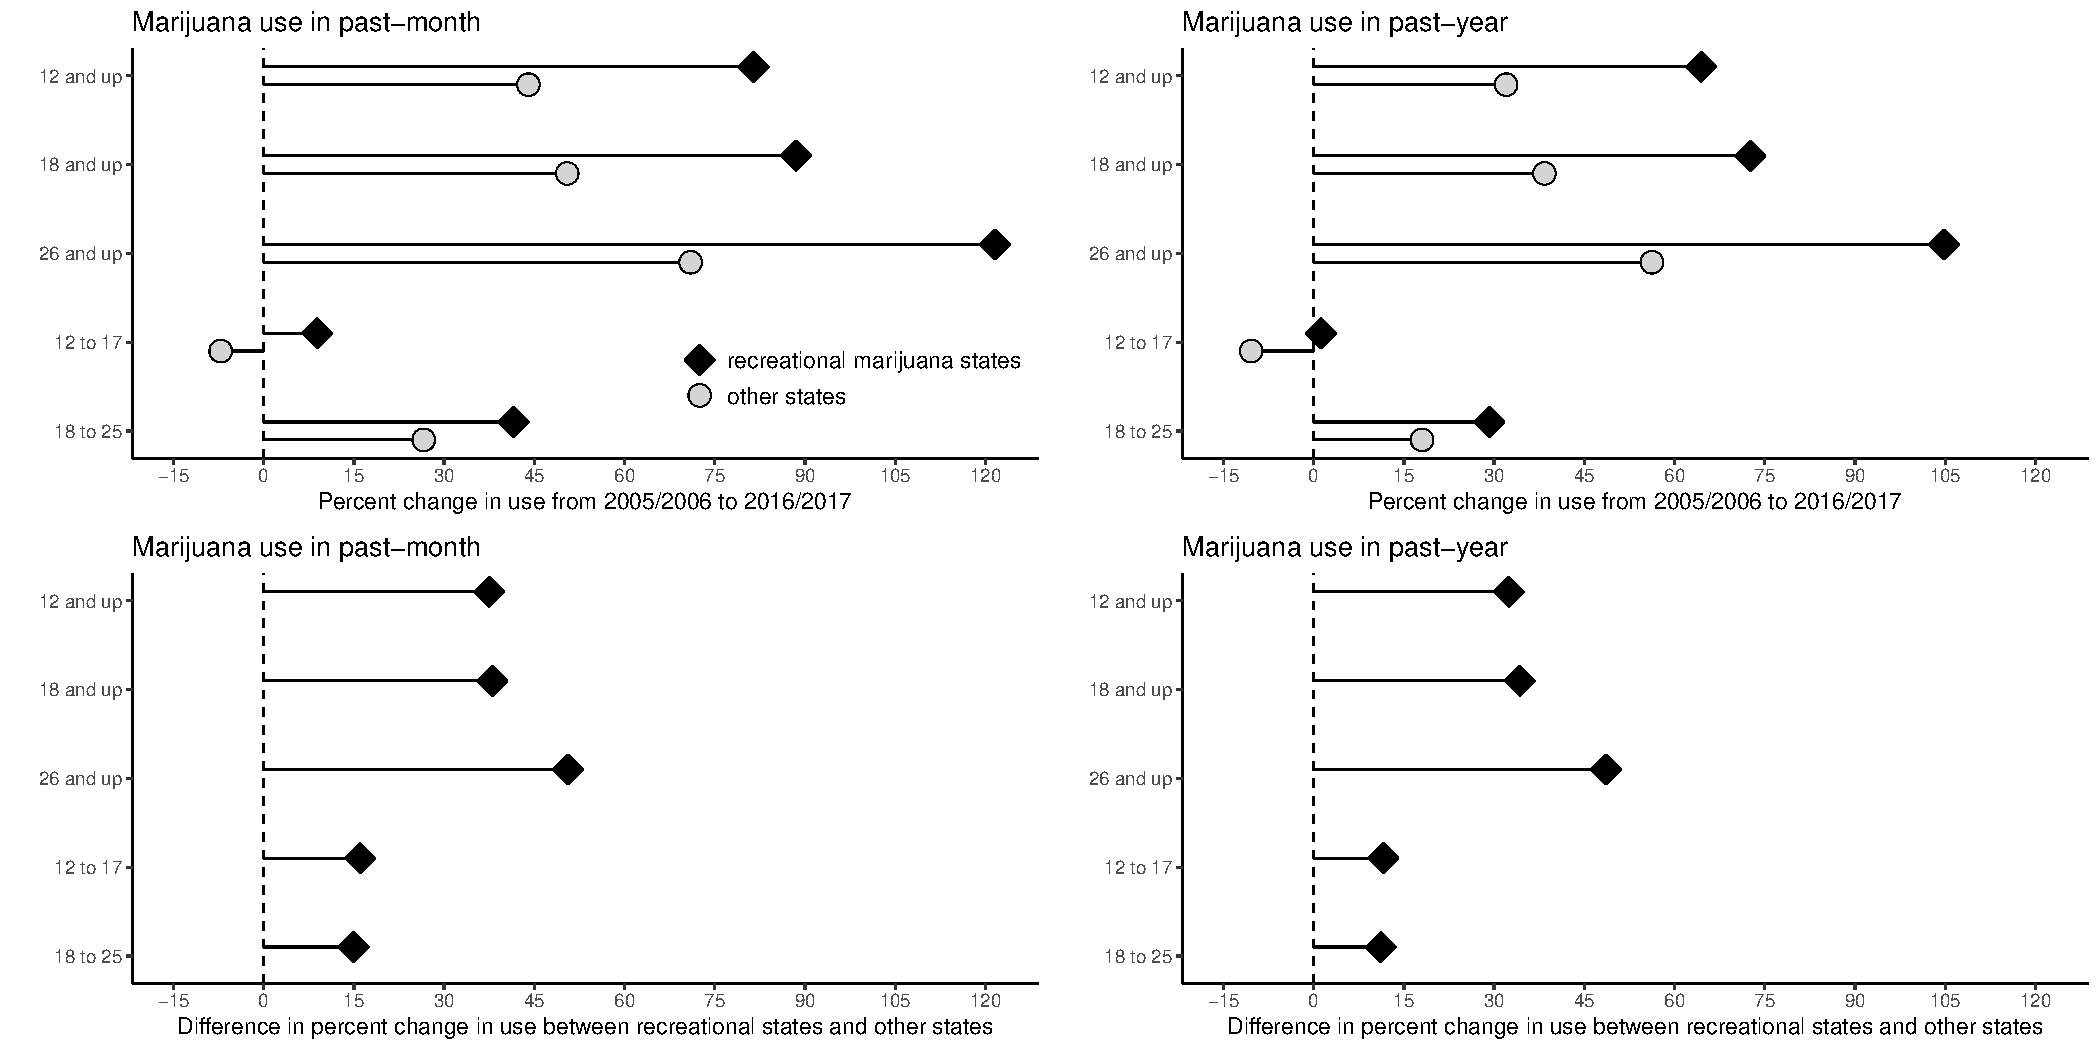
\includegraphics[width=\linewidth]{../output/plots/bw-change-in-use.pdf}
    \end{minipage}
        \label{fig:change-in-mj-use-percent}
\end{figure}

\paragraph{Event study analyses}
To test the assumption that the timing of the recreational marijuana laws are not associated with differential pre-treatment time trends, and to examine the way the effects of the laws change with time since adoption, we estimated an event study models that include indicator variables for the periods leading up to and lagging the policy changes in each state. Figures~\ref{fig:leads-and-lags-mj-past-year}-\ref{fig:leads-and-lags-mj-first-use} show the estimates for each measure of marijuana use from the event study regressions outlined in Equation~\ref{eq:event_study}. In each figure, the dependent variable is the natural log of the prevalence of drug use in state $s$ in period $t$ for a specified age group and type of drug. 
We use the model coefficients to compute $\% \Delta \approx 100\times \left[exp(\beta_1)-1\right]$, which is the percent change in the prevalence of drug use generated a given policy change.  
The shaded area reports 95\% confidence intervals. 

For each outcome and age group, the coefficients on the recreational marijuana leading dummies are small and stable across time, which lends credibility to our assumption that differential pre-trends are not driving the results. In contrast, the coefficients on the post-recreational marijuana lags are typically large and positive. For measures of past-year marijuana use and first time marijuana use, the point estimates suggest that the effects of the recreational marijuana laws on marijuana use increased with time since adoption. However,  this increasing trend should not be over-interpreted as the confidence intervals on the post-adoption coefficients overlap with one another so that the data are also consistent with a constant treatment effect. The post-period event study coefficients are statistically different from zero for most periods and outcomes for adults, but the point estimates are smaller and noisier for adolescents. 

The growing treatment effect observed in the event-study specifications could be in part due to marijuana dispensaries, which tend to open a few years after recreational marijuana is legalized for consumption and possession. We evaluated possibility this using Equation~\ref{eq:two_way_fe_disp}. The resulting coefficient estimates are presented in Table~\ref{tab:mj_use_add_rm_disp}. In these specifications, we regressed measures of log drug use prevalence on binary indicators for recreational, medical, medical-dispensary, and recreational-dispensary laws; a vector of time varying covariates; state fixed effects; and census region-by-year fixed effects.\footnote{The vector of time varying covariates includes state-level unemployment rate, median income, \% white, and \% male in each state-year} 

In each specification, the dependent variable is the natural log of the prevalence of drug use in state $s$ in period $t$ for a specified age group and type of drug. We use the model coefficients to compute $\% \Delta \approx 100\times \left[exp(\beta_1)-1\right]$, which is the percent change in the prevalence of drug use generated a given policy change.  We use a cluster robust variance matrix that allows for dependency at the state level to estimate standard errors for the coefficients, and we use the delta method to compute standard errors for the transformed coefficients. The standard errors are shown in parenthesis. The results that include dispensaries report the combined estimated treatment effect of legalization and  of dispensaries opening.  We compute the combined effect by adding the estimated coefficients on the binary indicator for medical (recreational) marijuana  and the binary indicator for medical (recreational) dispensary and then using the transformation above to compute the percentage effect. The standard error refers to the standard error of the combined effect. 

The table reports point estimates of the percent change in the prevalence of each measure of marijuana use for each age group. We find recreational marijuana legalization \emph{without} dispensary access increases marijuana use in every age group across all measures of use. For recreational adoption without dispensaries, the estimates show that past-year marijuana use rates increased by 11 percent among adolescents (ages 12-17), 12 percent among young adults (ages 18-25), and 13 percent among older adults (ages 26+). The effects of a non-dispensary recreational policy on past-month marijuana use are similar, with recreational legalization increasing past-month marijuana use by 14 percent for adolescents, 16 percent for young adults, and 21 percent for older adults. Finally, recreational marijuana laws with no dispensary access increase the fraction of those who recently used marijuana for the first time by 15 percent for adolescents, 17 percent for younger adults, and 10 percent for older adults. 

%------------------------------------------%
%    Figure 2 - Leads and lags by use type
%------------------------------------------%
\begin{figure}[h]
    \caption{Event-study estimates showing the impact of recreational marijuana legalization on marijuana use in the past year by age group.}
    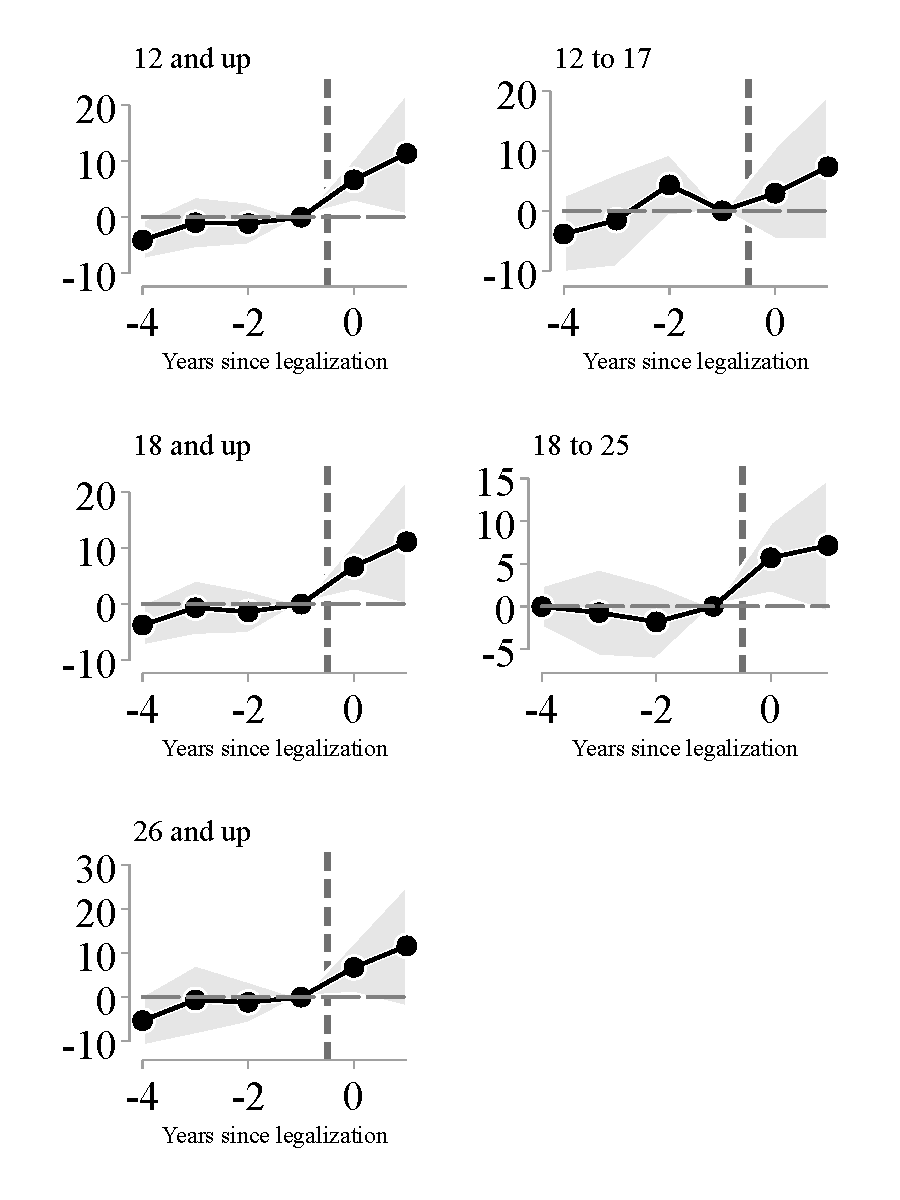
\includegraphics[width=.75\linewidth]{../output/plots/bw-event-study-estimates-ln-mj_use_365-bw.pdf}
    \label{fig:leads-and-lags-mj-past-year}
\end{figure}

%------------------------------------------%
%    Figure 3 - Leads and lags by use type
%------------------------------------------%
\begin{figure}[h]
    \caption{Event-study estimates showing the impact of recreational marijuana legalization on marijuana use in the past month by age group.}
    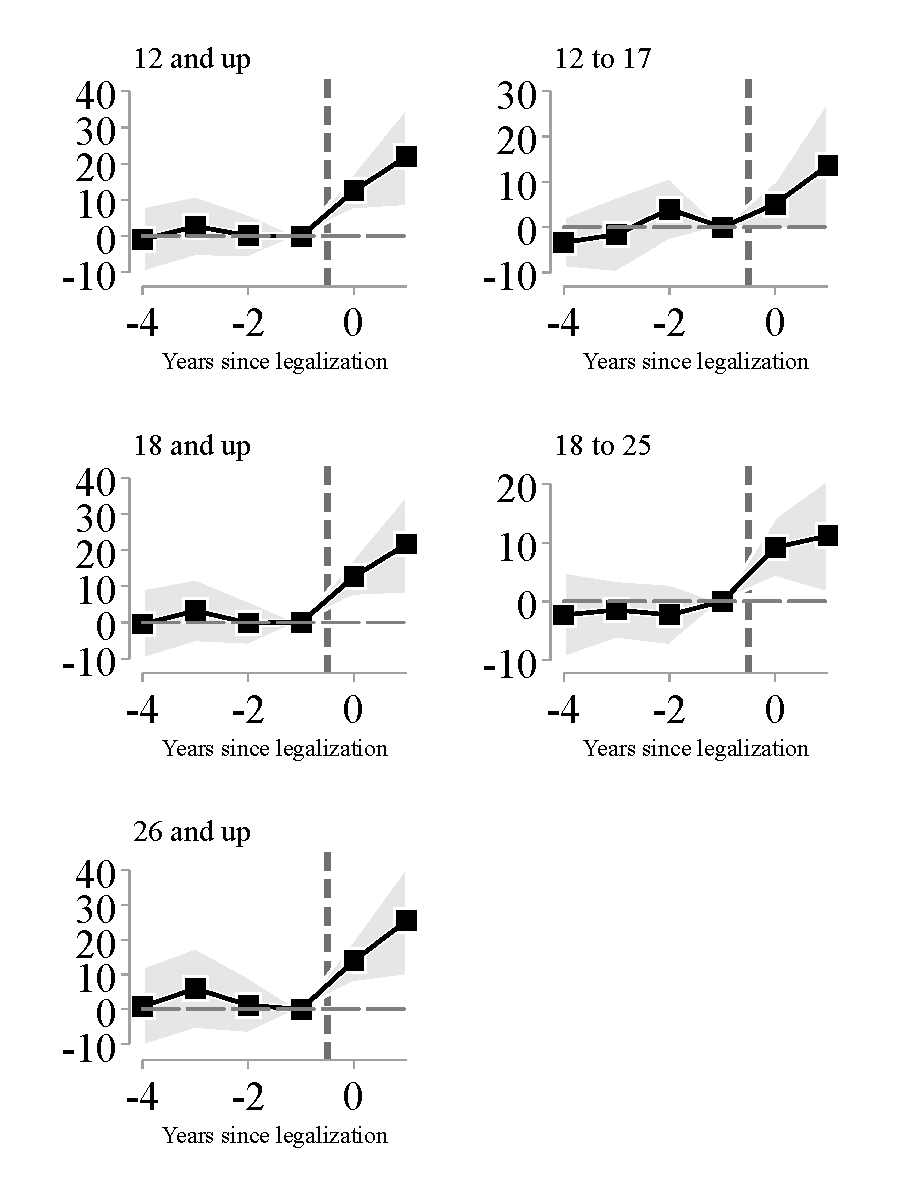
\includegraphics[width=.75\linewidth]{../output/plots/bw-event-study-estimates-ln-mj_use_30-bw.pdf}
    \label{fig:leads-and-lags-mj-past-month}
\end{figure}

%------------------------------------------%
%    Figure 4 - Leads and lags by use type
%------------------------------------------%
\begin{figure}[h]
    \caption{Event-study estimates showing the impact of recreational marijuana legalization on new marijuana initiates by age group.}
    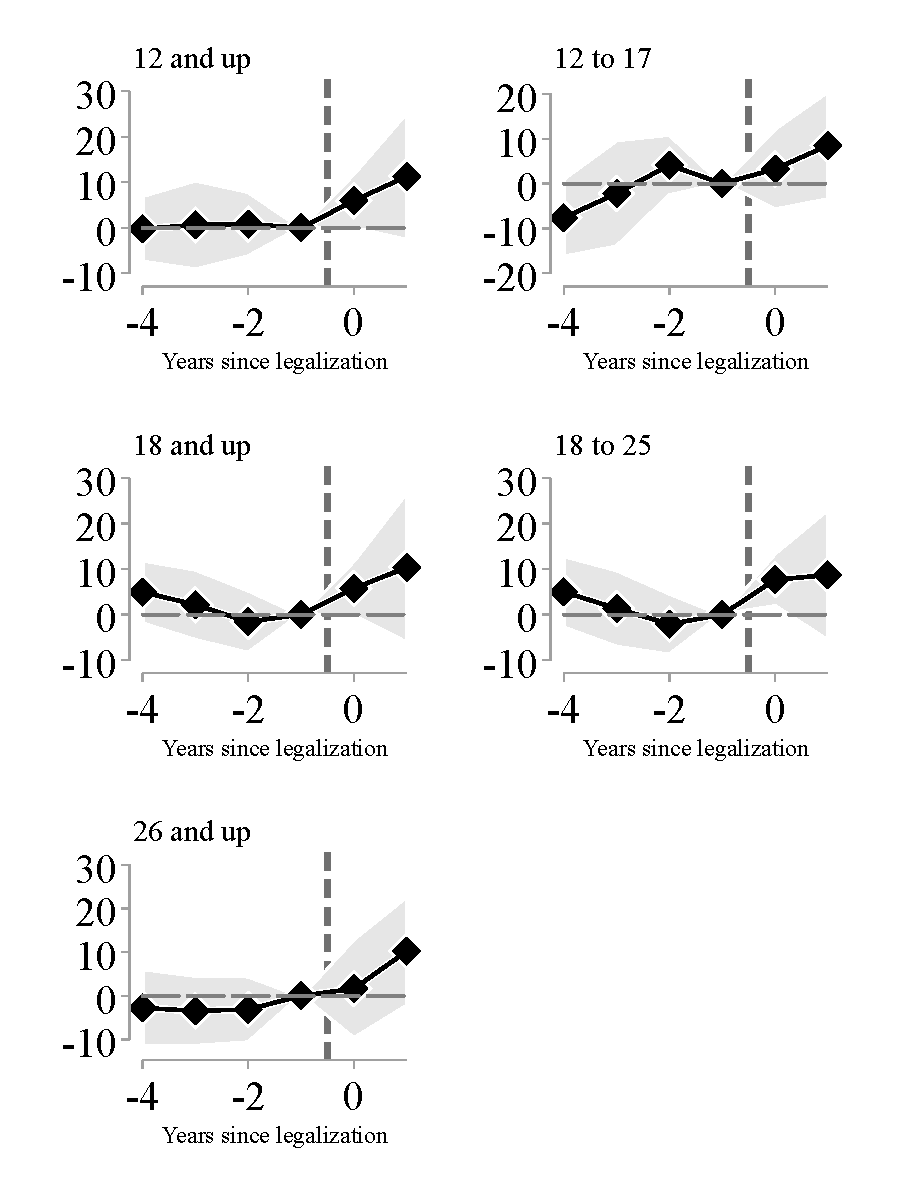
\includegraphics[width=.75\linewidth]{../output/plots/bw-event-study-estimates-ln-mj_first_use-bw.pdf}
    \label{fig:leads-and-lags-mj-first-use}
\end{figure}

\paragraph{Goodman-Bacon decompositions}
To estimate the effect of recreational marijuana laws in a more organized way, we fit the simple version of the two-way fixed effects regression model, which includes state and year fixed effects, and a recreational marijuana law indicator. 
Figure~\ref{fig:bacon_lead_lag_mj} shows the connection between the regression-based estimate of the effect of law and the nine pairwise DIDs that make up the design. 
In separate panels, we show the decomposition for three measures of marijuana use in five age groups.  In each graph, the vertical axis shows the treatment effect estimate measured as a percentage change in the prevalence of marijuana use. The horizontal axis measures the weight assigned to a particular pairwise DID comparison. Each of the scattered points in the graph gives the effect and weight associated with a different pairwise DID. The spacing of the scatter of points along the horizontal axis is identical across the graphs because the weights depend only on the sample share and adoption dates, which do not change across outcomes and age groups. The long-dashed line shows the coefficient estimate from the fixed effect regression model.
In each case, the fixed effect estimate – the weighted average of the pairwise DIDs – indicates that recreational laws generate substantial increases in marijuana use.

There are three important messages from the decomposition analysis in Figure~\ref{fig:bacon_lead_lag_mj}. First, the pooled fixed effects model puts the majority of the weight on comparisons of treated timing groups to the never treated group. In contrast, comparisons that exploit differential timing of adoption across pairs of treated timing groups receive much less weight. Second, the point estimates are quite similar across the nine pairwise designs, which suggests that the effects of the recreational marijuana laws are not very heterogeneous and that the fixed effect framework gives a reasonable summary effect measure. In particular, the three heavily weighted DIDs have quantitatively similar treatment effect estimates for most of the measures of marijuana use and in most of the age groups. Most of the timing-based DIDs are also clustered close to the regression-based estimate. Third, the most discrepant pairwise DIDs are timing-based comparisons that use an already treated unit as a control and a later treated group as a treatment group. The estimates from these DIDs are closer to zero and are occasionally negative. This may indicate that treatment effects change somewhat with time since adoption and that this leads to violations of the common trend assumption for these pairwise DIDs. This late vs early timing group problem is apt to be a negligible  source of bias in our study because these problematic DIDs receive little weight in the two-way fixed effects formulation.

\paragraph{Two-way fixed effects models}
Our main set of results come from the model in Equation~\ref{eq:two_way_fe}, which jointly examines the effects of recreational laws, medical laws, and medical dispensaries. Figure~\ref{fig:main_coef_plot} reports the coefficient estimates of the effect of recreational marijuana legalization on marijuana use by age group across three specifications of the basic model. The circles show the effect of recreational laws on marijuana use in the past year, the squares are the effects on marijuana use in the past 30 days, and the triangles show effects on the proportion of people who used marijuana for the first time in the past two years. We show estimates from three specifications: the open markers show effects from a model with only state and year fixed effects, the shaded markers add time varying covariates, and the solid markers add census region-by-year fixed effects. This third model is the same as Equation~\ref{eq:two_way_fe}. 

Across all models, the dependent variable is the natural log of the prevalence of drug use in state $s$ in period $t$ for a specified age group and type of drug. We use the model coefficients to compute $\% \Delta \approx 100\times \left[exp(\beta_1)-1\right]$, which is the percent change in the prevalence of drug use generated a given policy change.  We use a cluster robust variance matrix that allows for dependency at the state level to estimate standard errors for the coefficients, and we use the delta method to compute standard errors and associated 95\% confidence intervals that are reported in brackets. 

The point estimates are very stable across the three specifications and they imply that recreational marijuana laws increase marijuana use substantially. The 95\% confidence intervals on these effects exclude zero for every age group and outcome measure. 
Using the results from the model with census region-by-year fixed effects, we find that past-year marijuana use rates increased by 11 percent among adolescents (ages 12-17), by 13 percent among young adults (ages 18-25), and by 18 percent among older adults (ages 26+). The effects on past-month marijuana use are similar albeit slightly larger, with recreational legalization increasing the prevalence of past-month marijuana use by 14 percent for adolescents, 16 percent for young adults, and 26 percent for older adults. Finally, recreational marijuana laws also increase the fraction of people who used marijuana for the first time in the past two years by 15 percent for adolescents, 20 percent for younger adults, and 19 percent for older adults.

For most age groups, the combined effect of legalization and dispensaries is not much different than the initial effect of legalization on its own. However, dispensaries seem to have a very large effect on adults aged 26 and older. Among adults 26 and older, access to a recreational dispensary increases the effect of the recreational marijuana law on past-month use by half, doubles the effect on the prevalence of past-year marijuana use, and triples the increase in the prevalence of those who recently tried marijuana for the first time. For the two age groups that do not include those aged 26 and over, access to a dispensary does increase marijuana use relative to legalization only, but the difference in magnitude between the effects is smaller.\footnote{In Appendix Table~\ref{tab:mj_use_aggressive}, we report similar results that use an aggressive timing variable following \citet{Friedman2015} and outlined in section~\ref{sec:data_laws}. With this timing definition the combined effect of recreational marijuana legalization and recreational dispensaries is at least twice as large as the effect of recreational marijuana legalization without dispensaries for almost every age group and measure of use.}

\subsection{Effects of Medical Marijuana Laws on Marijuana Use}
\label{sec:results_medical}

Table~\ref{tab:mj_use_add_rm_disp} also shows estimates of the effects of dispensary and non-dispensary medical marijuana laws on the same set of marijuana utilization outcomes. The results imply that dispensary-based medical marijuana laws also lead to increased marijuana use among adults. However, the effects of recreational marijuana laws are three to four times larger than the analogous estimates for dispensary-based medical marijuana laws. For example, medical laws with dispensaries increase past-month marijuana use by 9 percent for older adults, while the recreational effect is 3.6 times larger. 


Medical marijuana laws have small and more statistically imprecise effects on past-year adolescent marijuana use. There is some evidence that medical marijuana adoption increases past-month use and the likelihood of an adolescent trying marijuana for the first time. However, like the effects on adult use, the point estimates of the effects of recreational laws on adolescent marijuana use are at least three times larger than the point estimates of the effects of medical laws on adolescent marijuana use. Non-dispensary medical marijuana laws have smaller and less precisely estimated effects on the prevalence of marijuana use across all ages and measures of marijuana use than medical marijuana laws with dispensaries. The majority of the coefficients on non-dispensary medical marijuana laws are not statistically different from zero. 


\subsection{Effects of Marijuana Laws on Other Psychoactive Substance Use}
\label{sec:results_other}

We also examined the effect of medical and recreational marijuana legalization on the prevalence of any alcohol use in the previous month, any tobacco use in the previous month, and any cocaine use in the previous year. For each substance and age group, we follow the same four step research strategy we used to study marijuana use. We discuss the results here, but relegate the tables and figures to the appendix.

 Figure~\ref{fig:bacon_lead_lag_oth} presents the \cite{Goodman-Bacon2018} pairwise DID decomposition for studies of the effects of recreational marijuana laws on measures of alcohol, tobacco, and cocaine use. The weights in these decompositions are identical to the weights shown in Figure~\ref{fig:bacon_lead_lag_mj} for marijuana use, and the point estimates also tend to cluster around the pooled fixed effect estimates. Figure~\ref{fig:aux_coef_plot} plots the effect estimates and confidence intervals from two-way fixed effects regressions that do not distinguish between dispensary and non-dispensary recreational marijuana effects. The results suggest that recreational laws did not have a substantial effect on adult alcohol or tobacco consumption. In contrast, recreational marijuana may have increased the prevalence of cocaine use by about 10 to 12 percent among adults.

 Figure~\ref{fig:unbalanced_lead_lag_other} presents results of the event study analysis of the effects of recreational marijuana laws on use of alcohol, tobacco, and cocaine. There is no evidence of differential pre-trends or anticipation effects. The post-treatment coefficient estimates suggest that recreational marijuana laws did not affect the use of alcohol for any age group. There is some evidence that recreational adoption decreases adult tobacco consumption three years following adoption. As in the simple two-way fixed effects analysis, the event study results suggest that recreational laws increased cocaine use. These event study point estimates are noisy, but they do increase substantially over the first two years after recreational marijuana laws for all age groups. The effects on cocaine use are statistically significant in the second post-treatment year for all of the samples that include the older adults.   

Finally, Table~\ref{tab:other_use_add_rm_disp} shows estimates of the effects of recreational marijuana laws on rates of alcohol use in the past month, tobacco use in the past month, and cocaine use in the past year for each of the five age groups using our preferred specification, which allows the effects of the recreational laws to change after dispensaries open. Here we see that non-dispensary medical marijuana laws reduce alcohol use by 1.5 percent for younger adults and by 2.0 percent for older adults. The point estimate is small and not statistically different from zero for adolescents, but the effects are significant for adult use. Dispensary based medical laws also seem to reduce alcohol use, although the estimates are noisier. In addition, we find that medical marijuana reduced the prevalence of tobacco consumption for adolescents and young adults, while dispensary based recreational laws appear to reduce tobacco consumption for older adults. 

These results also show that adult cocaine use appears to increase following recreational and medical marijuana legalization. The cocaine results are sensitive to specification choice, however. If we include population weights, all other results persist for recreational marijuana, but the effects of marijuana legalization on cocaine use become indistinguishable from zero. 

\subsection{Effects of Marijuana Laws on Workplace Drug Test Positivity}
\label{sec:workplace_results}

Our analysis so far uses self-reported measures of the prevalence of drug use that are collected in the NSDUH. 
One drawback to this approach is that the survey data could be misleading if respondents do not give true and accurate answers to questions about their use of marijuana and other drugs. 
To help allay these concerns we examined non-survey data from workplace drug tests results reported by Quest Diagnostics. 
Specifically, we obtained data on the fraction of Quest Diagnostics workplace drug tests that were positive for tetrahydrocannabinol (THC)---the psychoactive component of marijuana---in each state-year from 2007 to 2019. 
Table \ref{tab:quest_regs} reports estimates of regressions of the log positivity rate on the marijuana policy variables using versions of the the specification in equation \ref{eq:two_way_fe_disp}, which allows the effect of the policies to change after dispensaries open. 
The baseline specification in column (1) includes state fixed effects and year fixed effects. 
Column (2) shows results from a model that includes a full set of census region by year fixed effects. 
The results imply that when states adopt a recreational marijuana law, the fraction of workplace drug tests that are positive for marijuana use rises by almost 18 percent. 
The positivity rate rises even more after dispensaries open. 
In total, adopting a recreational marijuana law and opening dispensaries increase the workplace marijuana test positivity rate by about 30 percent. 
Medical marijuana laws do not seem to affect the workplace test positivity rates. 

%------------------------------------------%
%    Figure 3 - MJ Use by RML Binary
%------------------------------------------%
\begin{figure}[h]
    \caption{The impact of recreational marijuana legalization on marijuana use by age group.}
    \begin{minipage}{\linewidth}
      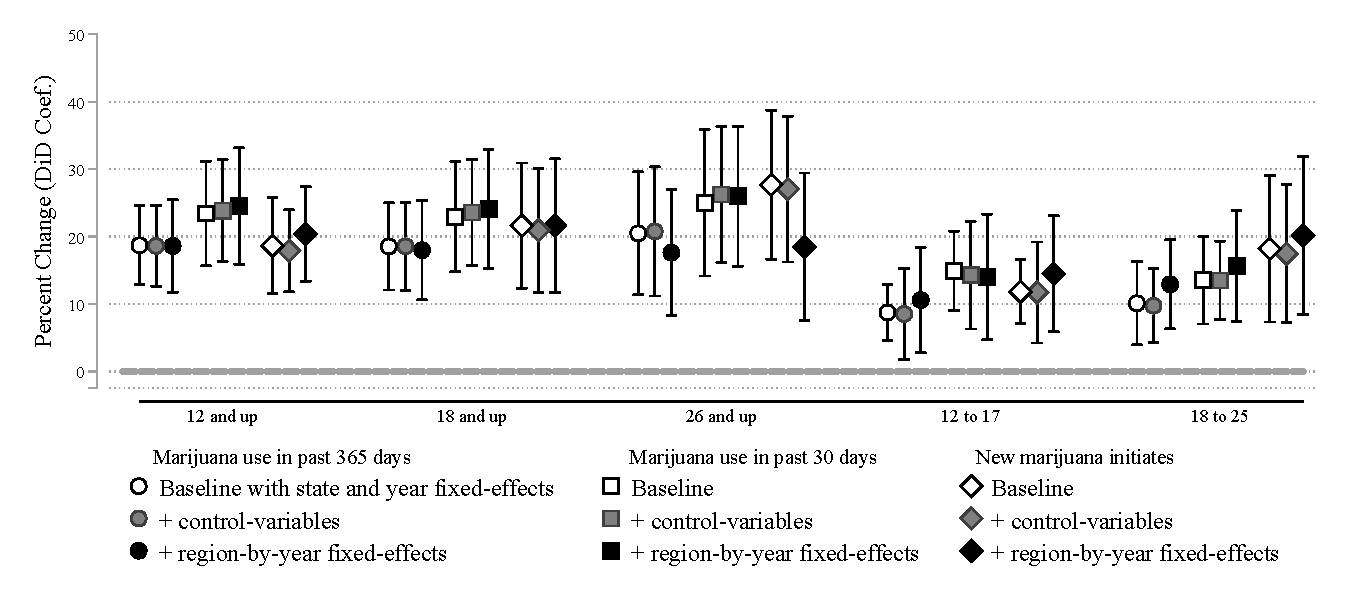
\includegraphics[width=\linewidth]{../output/plots/bw-main_recreational_figure_for_paper_robust_part_a.pdf}
       \label{fig:main_coef_plot}
    \end{minipage}
\end{figure}

%------------------------------------------%
%                Table 2
%------------------------------------------%
% Recreational marijuana and marijuana use
\begin{table}[h]\centering
    \begin{adjustbox}{width=.85\textwidth}
    \centering
      \begin{threeparttable}
        \caption{The impact of recreational marijuana on marijuana use by age group and frequency of use.}
        \estauto{../output/tables/mj_full_table_add_rm_disp.tex}{6}{S[table-format=1.2,table-column-width=20mm]}
        \label{tab:mj_use_add_rm_disp}
         \Fignote{
                 * p $<$ 0.1, ** p $<$ 0.05, *** p $<$ 0.01. Effects are in percent.  
                   }
      \end{threeparttable}
     \end{adjustbox}
\end{table}

%------------------------------------------%
%     Table 3: Quest diagnostic table
%------------------------------------------%
\begin{table}[t]\centering
    \begin{adjustbox}{width=.6\textwidth}
    \centering
      \begin{threeparttable}
        \caption{Access to recreational marijuana increases the percent of drug tests detecting THC.}
       \estauto{../output/tables/percent_test_positive_for_thc.tex}{3}{S[table-format=1.2,table-column-width=20mm, table-alignment = center]}
                    \label{tab:quest_regs}
         \Fignote{
          * p $<$ 0.1, ** p $<$ 0.05, *** p $<$ 0.01. Effects are in percent.  Data come from quest diagnostics and include years 2007 to 2019.}
      \end{threeparttable}
     \end{adjustbox}
\end{table}



Online Appendix Figure~\ref{fig:event-study-drug-tests} shows event study estimates of the effects of recreational marijuana laws on the log of the workplace marijuana positivity rate. 
In the figure, the x-axis denotes years since recreational adoption, with negative values indicating years prior to adoption. 
The specification includes indicators for the status of medical marijuana and medical dispensaries being open in each state and year, along with state and region-by-year fixed-effects.
To make the results more interpretable, we transform the event study coefficients to reflect percent changes and we compute standard errors on the transformation using the delta method. In the figure, the shaded area represents a 95\% confidence interval, calculated from robust standard errors clustered at the state level.

For the pre-treatment period all treatment estimates are statistically indistinguishable from zero and exhibit no problematic trends. 
This suggests that before recreational marijuana is adopted there is no difference between the THC positivity rates in states that will eventually adopt and all other states. 
Following adoption, there is a sharp rise in the percent of drug tests that indicate the presence of THC, with the point estimate hovering around 25\% in each year following recreational adoption. 

These workplace drug testing results should be interpreted with caution. 
Unlike the data from the NSDUH, the Quest Diagnostics workplace testing data can make no claim to being a random sample of firms or of workers or even of workers or firms that engage in workplace drug testing. 
At the same time, the results are consistent with the results from the NSDUH SAE data because they suggest that more people are using marijuana after states adopt recreational marijuana laws. 
Although the workplace testing data have their own problems of representativeness, they do not face the same concerns about possible changes in people's willingness to self-report their drug use. 
Taken together, the NSDUH SAE analysis and the workplace test positivity analysis suggest that recreational marijuana laws lead to a genuine increase in the prevalence of marijuana use.


%------------------------------------------%
%      Table 4: Drug Arrests Table         %
%------------------------------------------%
\begin{table}[ht]\centering
    \begin{adjustbox}{width=.7\textwidth}
    \centering
      \begin{threeparttable}
        \caption{The effect of marijuana legalization on arrests.}
      \estauto{../output/tables/mj_full_table_add_rm_disp_crime.tex}{3}{S[table-format=1.2,table-column-width=25mm]}
      \label{tab:arrest_poisson}
      \Fignote{
         * p $<$ 0.1, ** p $<$ 0.05, *** p $<$ 0.01. 
    Data come from the UCR and include years 2000 to 2016.  } 
      \end{threeparttable}
     \end{adjustbox}
\end{table}

\subsection{Effects of Marijuana Laws on Marijuana Arrests}
\label{sec:arrest_results}


We also examined the effects of state marijuana laws on the number of juvenile and adults marijuana related arrests using data from the FBI Uniform Crime Reports (UCR). We estimate the effects of the marijuana policies using a fixed effects Poisson regression based on the model in Equation \ref{eq:two_way_fe_disp}. The results are in table \ref{tab:arrest_poisson}. 
Estimates for marijuana arrests among adults are in the top panel. The bottom panel has results for juveniles. 
All models adjust for state fixed effects and census region-by-year fixed fixed effects, which are inclusive of year fixed-effects. 
Like the other tables in the paper, the results from these  regressions are transformed to show the effects on a percentage scale. 
We use a cluster robust variance matrix that allows for dependency at the state level to estimate standard errors for the coefficients, and we use the delta method to compute standard errors for the transformed coefficients. The standard errors are shown in parenthesis. The results that include dispensaries report the combined estimated treatment effect of legalization and  of dispensaries opening.  We compute the combined effect by adding the estimated coefficients on the binary indicator for medical (recreational) marijuana  and the binary indicator for medical (recreational) dispensary and then using the transformation above to compute the percentage effect. The standard error refers to the standard error of the combined effect. The regressions adjust for unemployment rate, median income, \% white, and \% male.

Since these data are from arrests, our treatment effect estimates may represent a combination of changes in the prevalence of marijuana use and changes in police enforcement effort. 
For adults, we expect that recreational legalization should reduce arrests for marijuana possession even if use of the substance is increasing. 
Adult possession arrests may not fall all the way to zero since the federal government still considers marijuana to be a controlled substance and certain types of possession (e.g., adults below the age of 21 or possession of too great a quantity) are still illegal at the state level. It is unclear what to expect for adult sales arrests.
On the one hand we may expect a reduction since increased legal access may compete with previously illicit sales, and  police practices may change lessening focus on marijuana. 
However on the other hand, sales arrests could increase since access to marijuana to be ``re-sold'' increases after dispensaries open and this reselling is illegal. 

The results in table \ref{tab:arrest_poisson} suggest that, for adults, recreational marijuana laws led to large reductions in the number of arrests police agencies made for both possession and sales. 
The results for possession are consistent with our hypothesis that recreational legalization will reduce possession arrests. 
We similarly find that sales arrests decline, although we cannot  identify the precise mechanism as this could be due to the emergence of a competitor (legal marijuana) or due to changes in policing. 

For juveniles, the hypothesized effects of recreational legalization on both possession and sales arrests are unclear. 
It could be that changes in policing cause reductions in arrests for both possession and sales. However, it is also plausible that increased access to marijuana leads to more youth consumption and sales and thus increased arrests since both youth possession and sales are illegal even following recreational legalization.  
Difference in difference models suggest that juvenile arrests for possession of marijuana did not change when recreational marijuana was first legalized, but rose by 60\% after dispensaries opened. 
In contrast, we find negative, but statistically insignificant, point estimates on effect for juvenile arrests for selling marijuana.
These results are consistent with the idea that following the opening of a recreational dispensary, access to marijuana increases for adolescents despite marijuana possession for this age group remaining illegal. 

\subsection{Robustness Checks and Sensitivity Analysis}

We conducted a series of supplementary analyses to probe the sensitivity of our results to key threats to validity. 
We start by examining whether the statistical significance of our results is sensitive to different approaches of conducting statistical inference that rely on weaker assumptions about the error structure of the model. 
We do this by estimating sampling distributions under the null hypothesis of no effect using two procedures based on randomization inference. 
This allows for observations that are dependent within state, but are less prone to over rejecting the null hypothesis than cluster robust standard errors. 
Table \ref{fig:randomization_table} shows that the randomization inference p-values are not meaningfully different from the p-values obtained from tests based on clustered standard errors. 

We then give a short summary of a series of robustness checks used to examine if the structure of the NSDUH SAE data affects our results by dropping every other year (Table  \ref{tab:mj_full_table_add_rm_disp_drop_odd}), comparing the NSDUH to other survey measures of drug use (Figure \ref{fig:yrbs_nsudh_monthly}), using alternative coding of state law changes (Tables~\ref{tab:mj_use_aggressive} and~\ref{tab:other_use_aggressive}), and different model specifications (Tables~\ref{tab:mj_use_pop_weights}, ~\ref{tab:other_use_pop_weights}, ~\ref{tab:mj_use_pop_mean}, and~\ref{tab:other_use_pop_mean}).  Overall, the supplementary analyses all support our main conclusion. 

We then run a series of robustness checks not related to the NSDUH structure. 
First, we show that marijuana policy changes were not associated with changes in the composition of states over time following a procedure described in \citet{Pei2019} (Table~\ref{tab:covariate_balance_table}). 
Next, we show suggestive evidence indicating that the regions where recreational and medical marijuana law adopting states are located had changing population patterns, but the adopting states did not have differential population changes relative to their respective regions (Table~\ref{tab:mj_and_pop}). We assess concerns that recreational marijuana states may have had higher marijuana use even before the policy changes, leading to relatively faster growth rates, by constructing comparison groups that were matched on pre-treatment outcome levels for each outcome and age group (Tables~\ref{tab:mj_use_only_good_pretrends} (marijuana) and ~\ref{tab:other_only_good_pretrendss} (other drugs)).  Tables~\ref{tab:only_good_pretrends_list_mj} and~\ref{tab:only_good_pretrends_list_oth} list the states included in each restricted regression. Finally, in Tables~\ref{tab:mj_use_no_region_fe} to~\ref{tab:oth_use_division-by-year}, we estimate regulatory effects from models that impose both stronger and weaker forms of the common trends assumption. The estimated
effects of recreational marijuana and medical marijuana legalization on marijuana use are virtually unchanged across these different specifications


%------------------------------------------%
%      Conclusion                          %
%------------------------------------------%
    
\section{Conclusion} 
\label{sec:Conclusion}

The landscape of marijuana policy is changing. Federal law classifies marijuana as a Schedule I drug with no accepted medical use. State medical marijuana laws challenge this view and create ways that people can access marijuana to legally treat specific health conditions. Recreational marijuana laws further chip away at prohibition by sidestepping medical questions. Both types of laws reduce certain barriers to the consumption of marijuana. However, they also incorporate taxes, licenses, inspections, and age restrictions in an effort to control the availability of legal marijuana and discourage marijuana consumption. These policy changes are happening quickly, and more changes are on the horizon.

The evidence we report suggests caution may be in order. We find that recreational marijuana laws substantially increase marijuana use. When states adopt recreational marijuana laws with dispensaries, the fraction of adults over age 18 who report using marijuana in the past month increases by 30 percent. 
This is a large change in the prevalence of regular psychoactive substance use. The long run effects of changes in the popularity of drug use are hard to predict. 
For example, the current opioid epidemic has been highly damaging to individuals and communities, and that epidemic seems to have at least some roots in changing views about the acceptable medical uses and risks of opioid pain medications. 
While marijuana is safer and less addictive than opioids, our analysis nevertheless suggests that recreational marijuana laws are creating an equilibrium in which a greater share of the population uses intoxicating substances.  
While it is not clear how recreational laws affect  the timing and intensity of marijuana use,
future research should examine the way recreational marijuana laws affect performance at work, school, and home.

Our study suggests that the strategies states are using to control underage access to marijuana may not be effective. When states adopt recreational marijuana laws with dispensaries, the fraction of adolescents who report using marijuana in the past month increases by 15 percent. The medical community has raised concerns that marijuana use may be damaging for children and adolescents who are still undergoing neurological development. Even if these developmental concerns are disregarded, increases in child and adolescent drug use are an unappealing side effect of recreational marijuana laws. Many of these worries are amplified by the fact that existing laws do not restrict marijuana potency, and recreational marijuana markets tend to sell highly potent marijuana. Understanding the consequences of adolescent marijuana use and the effects of more potent marijuana is an important area for future work.

Although our work suggests that recreational marijuana laws may not be successful at restricting adolescent access, we do find evidence that medical marijuana markets may serve a gatekeeping function. That is, medical laws do not lead to large increases in marijuana use in the general population. These results undermine claims that medical marijuana laws are de facto recreational laws \citep{Anderson2014}. Medical marijuana laws might control recreational use because medical authorization procedures are difficult to fake. Alternatively, potential recreational users may be discouraged from falsifying applications because they are reluctant to engage in deception or unwilling to endure certification costs. In any case, developing a better understanding of the methods available to states to control access to marijuana is crucial as the marijuana policy experiment continues.
  
%------------------------------------------%
%       References
%------------------------------------------%      
\FloatBarrier
\newpage
\setlength{\bibsep}{0.0pt}
\begin{spacing}{0}
\bibliographystyle{references/econ}
\bibliography{references/rml_use_references.bib}{}
\end{spacing}

\newpage

%------------------------------------------%
%       Appendix for Publication
%------------------------------------------%
\FloatBarrier
\setcounter{page}{1}

\renewcommand*{\thepage}{A\arabic{page}}

% Reset figure/table #'s
\setcounter{table}{0}
\setcounter{figure}{0}


% Add an A in front of tables and figures
\renewcommand{\thetable}{A\arabic{table}}
\renewcommand{\thefigure}{A\arabic{figure}}
\renewcommand{\thesection}{A.\arabic{section}}
\renewcommand{\thesubsection}{A.\arabic{subsection}}

\FloatBarrier


\begin{appendices}
\begin{center}
    \noindent{\Large \textbf{Appendix}}
\end{center}

\addtocontents{toc}{\protect\setcounter{tocdepth}{3}}


\FloatBarrier

%------------------------------------------%
%                Table A1
%------------------------------------------%
%\begin{landscape}

\begin{table}[htp!]
\caption{Policy adoption years and timing groups.}
\begin{adjustbox}{width=\textwidth}
\begin{tabular}{@{}lccclcccc@{}}
\toprule
              & \multicolumn{3}{c}{Medical}                                                                         &  & \multicolumn{4}{c}{Recreational}                                             \\ \cmidrule(lr){2-4} \cmidrule(l){6-9}
State         & Law passed & Year First Legal                           & Year First Dispensary Opens               &  & Law passed & Year First Legal   & Timing Group & Year First Dispensary Opens \\ \midrule \midrule
Alaska        & 1998       & 1999 (1999 - 2000)                         & 2016 (2016-2017)                          &  & 2014       & 2015 (2015-2016)   & Mid          & 2016 (2016-2017)            \\
Arizona       & 2010       & 2010 (2010 - 2011)                         & 2012 (2012-2013)                          &  &            &                    &              &                             \\
Arkansas      & 2016       & 2016 (2016 - 2017)                         &                                           &  &            &                    &              &                             \\
California    & 1996       & 1996 (1996 - 1997)                         & 1996 (1996-1997)                          &  & 2016       & 2016 (2016 - 2017) & Late         & 2018 (NA)                   \\
Colorado      & 2000       & 2000 (2000 - 2001)                         & 2005 (2005-2006)                          &  & 2012       & 2012 (2012 - 2013) & Early        & 2014 (2014 - 2015)          \\
Connecticut   & 2012       & 2012 (2012 - 2013)                         & 2014 (2014-2015)                          &  &            &                    &              &                             \\
Delaware      & 2011       & 2011 (2011 - 2012)                         & 2015 (2015-2016)                          &  &            &                    &              &                             \\
D.C.          & 2010       & 2010 (2010 - 2011)                         & 2013 (2013-2014)                          &  & 2014       & 2015 (2015 - 2016) & Mid          &                             \\
Florida       & 2016       & 2017 (NA)                                  & 2016 (2016-2017)\sym{**} &  &            &                    &              &                             \\
Hawaii        & 2000       & 2000 (2000 - 2001)                         & 2017 (NA)                                 &  &            &                    &              &                             \\
Illinois      & 2013       & 2014 (2014 - 2015)                         & 2015 (2015-2016)                          &  & 2019       & 2020 (NA)          & NA           &                             \\
Louisiana     & 2016       & 2016 (2016 - 2017)                         & 2019 (NA)                                 &  &            &                    &              &                             \\
Maine         & 1999       & 1999 (1999- 2000)                          & 2011 (2011-2012)                          &  & 2016       & 2017 (NA)          & NA           &                             \\
Maryland      & 2003       & 2014 (2014 - 2015)\sym{*} & 2017 (NA)                                 &  &            &                    &              &                             \\
Massachusetts & 2012       & 2013 (2013 - 2014)                         & 2015 (2015-2016)                          &  & 2016       & 2016 (2016 - 2017) & Late         & 2018 (NA)                   \\
Michigan      & 2008       & 2008 (2008 - 2009)                         & 2009 (2009-2010)                          &  & 2018       & 2018 (NA)          & NA           &                             \\
Minnesota     & 2014       & 2014 (2014 - 2015)                         & 2015 (2015-2016)                          &  &            &                    &              &                             \\
Missouri      & 2018       & 2018 (NA)                                  &                                           &  &            &                    &              &                             \\
Montana       & 2004       & 2004 (2004 - 2005)                         & 2009 (2009-2010)                          &  &            &                    &              &                             \\
Nevada        & 2001       & 2001 (2001 - 2002)                         & 2015 (2015-2016)                          &  & 2016       & 2017 (NA)          & NA           & 2017 (NA)                   \\
New Hampshire & 2013       & 2013 (2013 - 2014)                         & 2016 (2016-2017)                          &  &            &                    &              &                             \\
New Jersey    & 2010       & 2010 (2010 - 2011)                         & 2012 (2012-2013)                          &  &            &                    &              &                             \\
New Mexico    & 2007       & 2007 (2007 - 2008)                         & 2009 (2009-2010)                          &  &            &                    &              &                             \\
New York      & 2014       & 2014 (2014 - 2015)                         & 2016 (2016-2017)                          &  &            &                    &              &                             \\
North Dakota  & 2016       & 2016 (2016 - 2017)                         & 2019 (NA)                                 &  &            &                    &              &                             \\
Ohio          & 2016       & 2016 (2016 - 2017)                         & 2019 (NA)                                 &  &            &                    &              &                             \\
Oklahoma      & 2018       & 2018 (NA)                                  & 2018 (NA)                                 &  &            &                    &              &                             \\
Oregon        & 1998       & 1998 (1998 - 1999)                         & 2009 (2009-2010)                          &  & 2014       & 2015 (2015 - 2016) & Mid          & 2015 (2015 - 2016)          \\
Pennsylvania  & 2016       & 2016 (2016 - 2017)                         & 2018 (NA)                                 &  &            &                    &              &                             \\
Rhode Island  & 2006       & 2006 (2006 - 2007)                         & 2013 (2013-2014)                          &  &            &                    &              &                             \\
Utah          & 2018       & 2018 (NA)                                  &                                           &  &            &                    &              &                             \\
Vermont       & 2004       & 2004 (2004 - 2005)                         & 2013 (2013-2014)                          &  & 2018       & 2018 (2018- 2019)  & NA           &                             \\
Washington    & 1998       & 1998 (1998 - 1999)                         & 2014 (2014-2015)                          &  & 2012       & 2012 (2012 - 2013) & Early        & 2014 (2014 - 2015)          \\
West Virginia & 2017       & 2019 (NA)                                  &                                           &  &            &                    &              &                             \\ \bottomrule
\end{tabular}
\label{tab:adoption_table}
\end{adjustbox}
{\footnotesize
    \begin{justify}
        \emph{Note}:
        In parentheses after each year, we report the first two-year NSDUH SAE data  that we consider treated in our preferred analysis.
        We adopt a conservative approach where we only consider a two-year period to be treated if both years have a particular policy in effect.
        Thus if a law was passed in 1999, we would consider 1998-1999 to be untreated and 1999-2000 to be treated.
        We adopt this approach since it will serve to attenuate our estimates.
        We also consider a more aggresive definition of treatment in Tables~\ref{tab:mj_use_aggressive} and~\ref{tab:other_use_aggressive}.
        A timing group is characterized by the policy adoption year for recreational marijuana: early includes Colorado and Washington (panel wave 2012/2013); mid includes Alaska, Oregon, and Washington DC (panel wave 2015/2016); and late includes California and Massachusetts (panel wave 2016/2017). \\
    \sym{*}~~~Although Maryland passed a law on 5/22/2003 (effective 10/2/2003) that provided legal protections to patients for possession/use of marijuana, no supply source was identified in the law. Therefore, most studies do not recognize this first law, and do not code MD as having a medical marijuana law until the June 2014 law passed (Powell et al. 2018). \\
    \sym{**}~~~~Florida opened up a dispensary in June 2016 under a "right-to-try " law only for terminally ill patients, therefore it is not coded in the data as having a medical marijuana dispensary.
    \end{justify}
}
\end{table}

%------------------------------------------%
%    Figure 2 - MJ Goodman Bacon Weights
%------------------------------------------%
\begin{figure}
    \caption{Goodman-Bacon DID decomposition weights and treatment effects estimates of the impact of recreational marijuana legalization on marijuana use by age group.}
  \begin{minipage}{.9\linewidth}
  \begin{subfigure}[b]{0.32\columnwidth}
    \caption{\scriptsize{Marijuana use in past year}}
    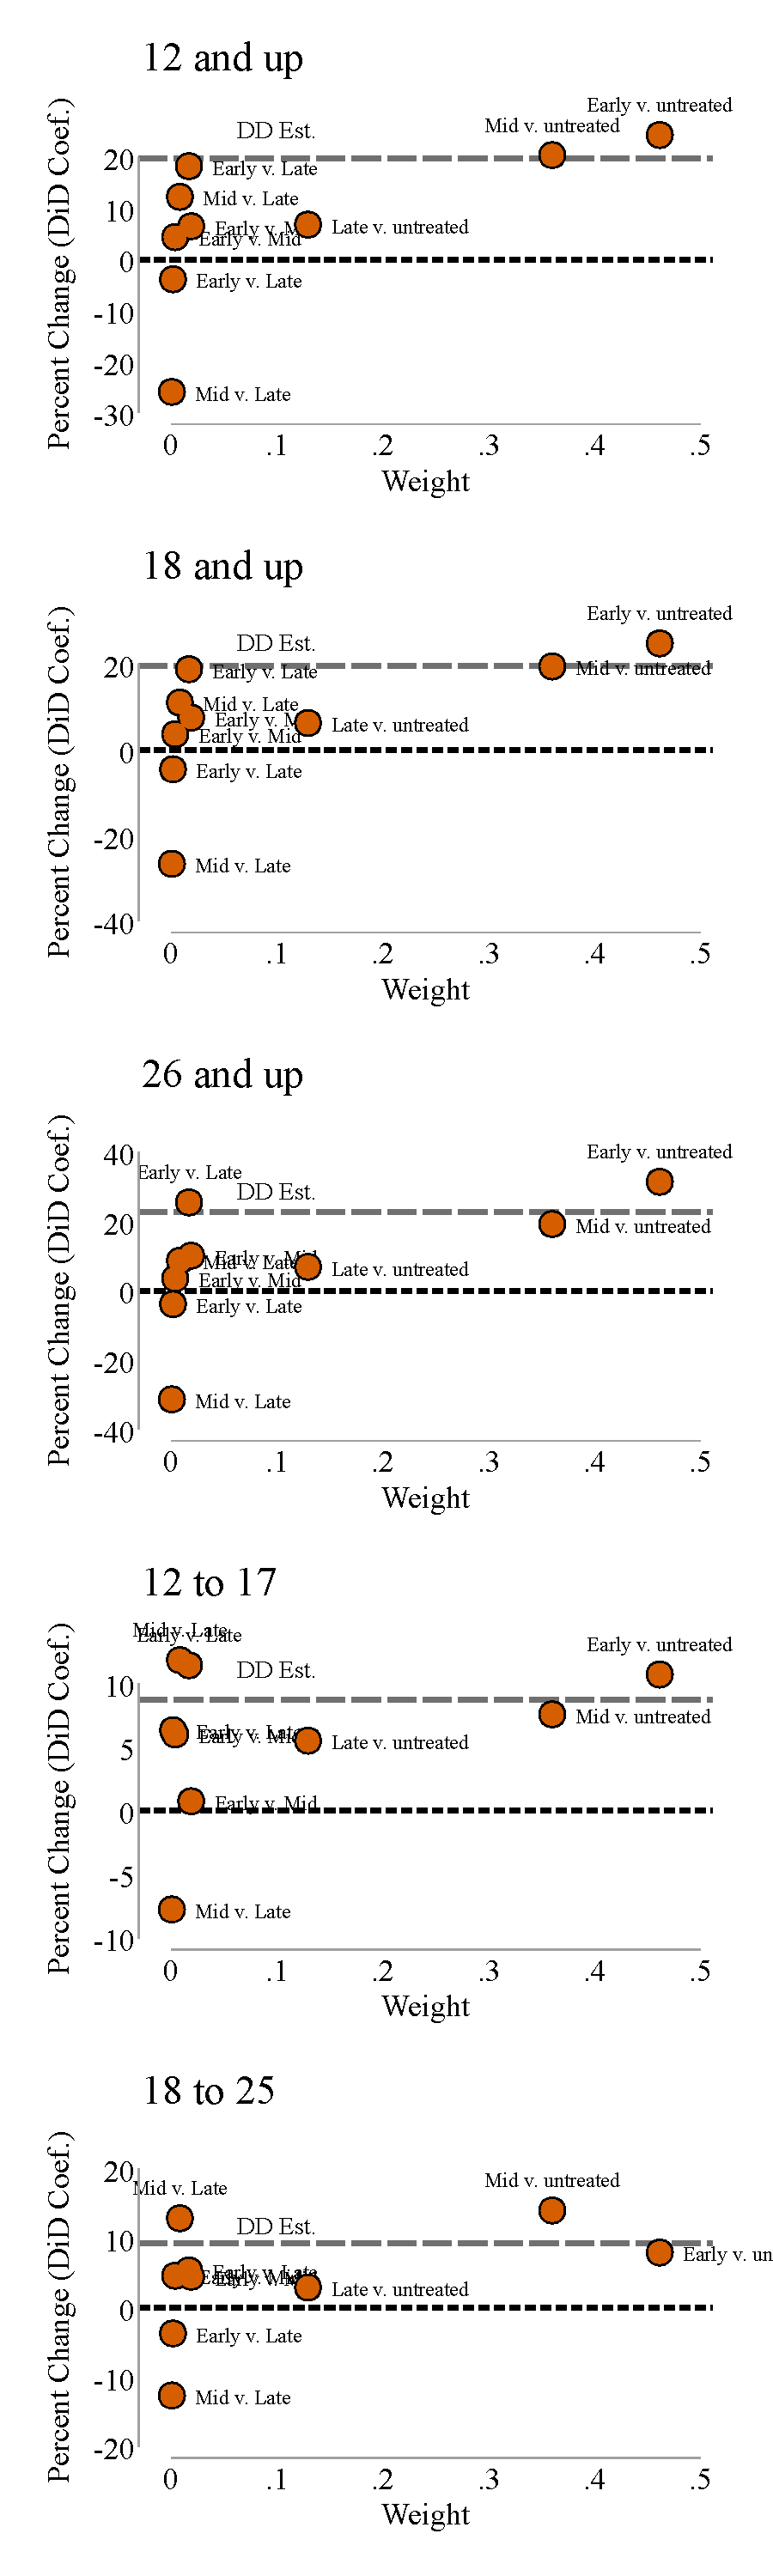
\includegraphics[width=\linewidth]{../output/plots/bacon_weights_ln_mj_use_365.pdf}
  \end{subfigure}
  \hfill %%
  \begin{subfigure}[b]{0.32\columnwidth}
      \caption{\scriptsize{Marijuana use in past 30 days}}
    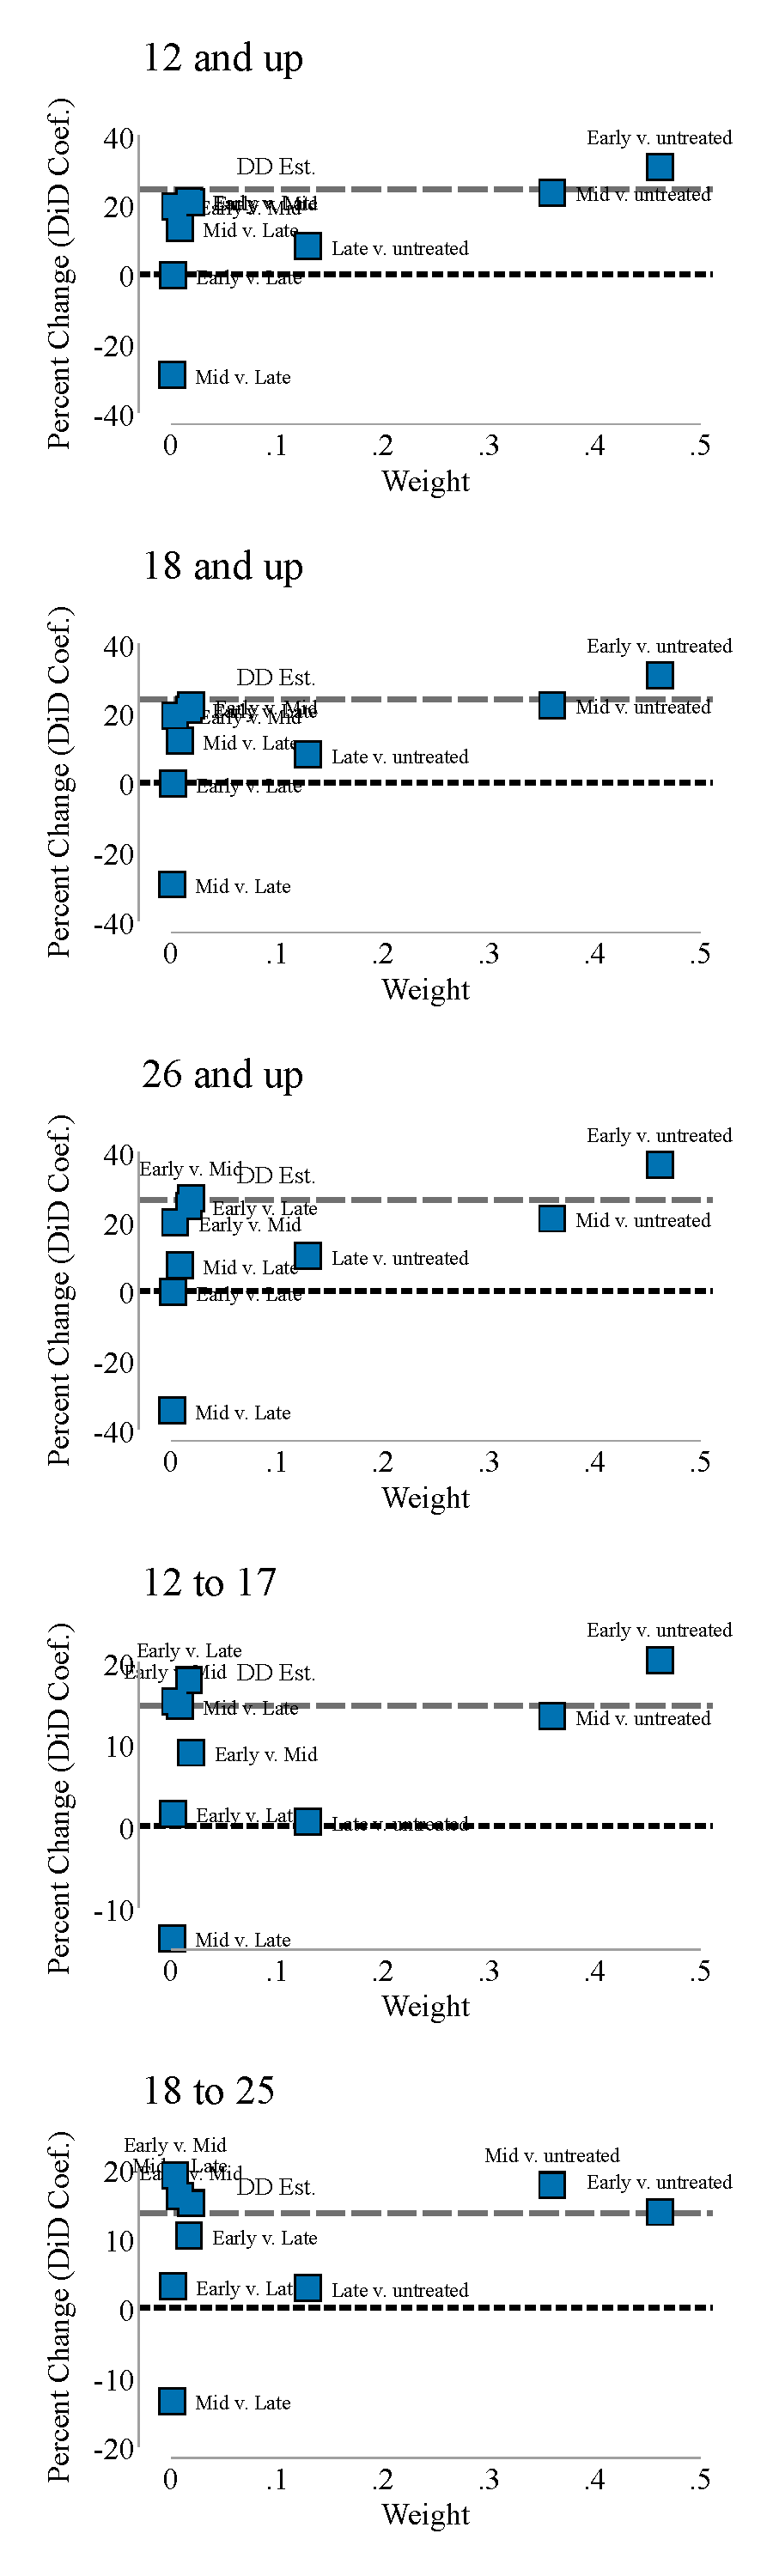
\includegraphics[width=\linewidth]{../output/plots/bacon_weights_ln_mj_use_30.pdf}
  \end{subfigure}
 \hfill %%
  \begin{subfigure}[b]{0.32\columnwidth}
      \caption{\scriptsize{Marijuana initiates in past two years}}
    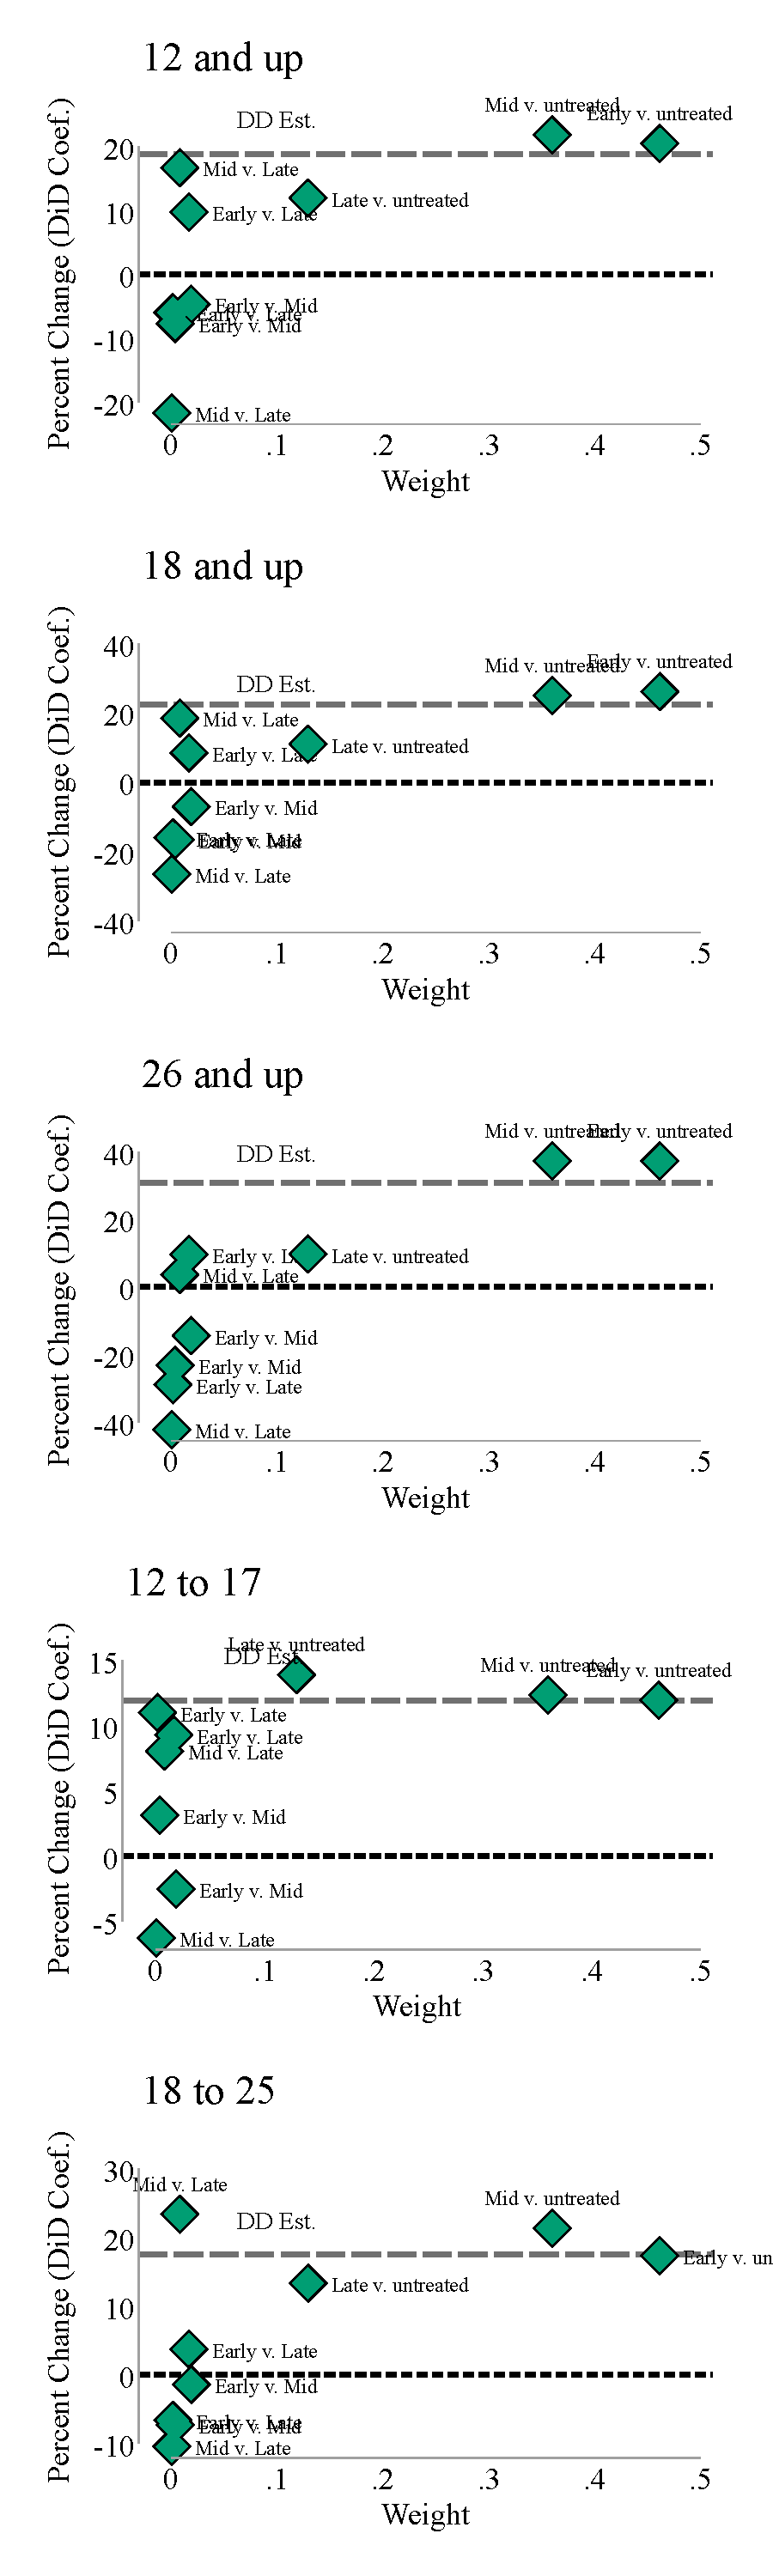
\includegraphics[width=\linewidth]{../output/plots/bacon_weights_ln_mj_first_use.pdf}
  \end{subfigure}
      \label{fig:bacon_lead_lag_mj}
         \begin{justify}
                {\footnotesize
                    \emph{Note:} 
            Weights are constructed as in \citep{Goodman-Bacon2018}.
            Each point plots the 2x2 DID coefficient from a comparison of the two groups in the label against the weight given to that group in the combined DID regression.
            The gray dashed line denotes the average DID treatment effect estimate and the black dashed line is at zero.
            The average DID treatment effect estimate reported here is the average of the y-values for each point weighted by their respective x-values.
            For ease of exposition, the regressions used to obtain these estimates include only state and year fixed-effects and do not control for other policy or control variables.
             We use the model coefficients to compute $\% \Delta \approx 100\times \left[exp(\beta_1)-1\right]$, which is the percent change in the prevalence of drug use generated a given policy change.    
                There are four total groups, one untreated group and three treated AKA timing groups (i.e. states that eventually adopt recreational marijuana laws).
            A timing group is characterized by the policy adoption year:
            early includes Colorado and Washington (panel wave 2012/2013);
            mid includes Alaska, Oregon, and Washington DC (panel wave 2015/2016);
            and late includes California and Massachusetts (panel wave 2016/2017).
                \par}
            \end{justify}
  \end{minipage}
\end{figure}

\end{appendices}
\newpage
%------------------------------------------%
%               Online Appendix
%------------------------------------------%
\FloatBarrier

%\pagenumbering{arabic}% resets `page` counter to 1
\setcounter{page}{1}

\renewcommand*{\thepage}{OA\arabic{page}}

% Reset figure/table #'s
\setcounter{table}{0}
\setcounter{figure}{0}

% Add an A in front of tables and figures
\renewcommand{\thetable}{OA\arabic{table}}
\renewcommand{\thefigure}{OA\arabic{figure}}
\renewcommand{\thesection}{OA.\arabic{section}}
\renewcommand{\thesubsection}{OA.\arabic{subsection}}

\FloatBarrier


%\begin{online_appendices}
% Make Table of Contents
\begin{center}
\noindent{\Large \textbf{Online Appendix}}


\end{center}

%%%%%%%%%%%%%%%%%%%%%%%%%%%%%%%%%%%%%%%%%%%%%%%%%%%%%%%%%%%%%%%%%%%%%%%%%%%%%%%%%%%%%%%
% Make an automatic table of contents

% Turn back on the storage of sections and subsections for the table of contents
\addtocontents{toc}{\protect\setcounter{tocdepth}{3}}


%-----------------------------------------%
%               Figure A1               %
%-----------------------------------------% 
\subsection{NSDUH and YRBS Comparison }\label{sec:yrbs_appendix}

An alternative source of survey data on adolescent drug use is the Youth Risk Behavior Survey (YRBS). A key difference between the YRBS and the NSDUH is the mode of data collection. The YRBS is school-based survey that is collected using a paper-and-pencil self administered questionnaire. The NSDUH is a household survey and the adolescent data are collected at the respondent's home. In theory, adolescent responses to both surveys may be affected by bystander effects. YRBS respondents may be answering questions in the presence of survey staff, teachers, other students. Adolescent NSDUH respondents may be answering questions in the presence of survey staff, parents, and siblings. 

Although the YRBS can be a useful data source, we believe that the NSDUH is a better choice for our study of the comparative effects of marijuana laws on drug use across age groups. The NSDUH offers the same measures of substance use for both adolescents and adults in each state over a period of time when states made changes to their marijuana laws, and the NSDUH sampling frame includes all adolescents and adults. In contrast, the YRBS does not include data from all states in any given year, and it only includes adolescents who are in school during survey collection.\footnote{There are actually several versions of the YRBS. The national YRBS is designed to provide a nationally representative sample of students but it is not meant to provide estimates at the sub-national level and it does not include students from all states in any given year. Some large school districts run a ``district level YRBS''. Most states also run a ``state level YRBS'', however several recreational marijuana states do not run a state level YRBS.  Research that combines these different national, state, and district surveys is quite complicated and weights that make them representative are not available.}%
These factors make it difficult to design credible difference-in-difference studies around the YRBS. 

Beyond these practical difficulties with the YRBS, the NSDUH also relies on more sophisticated methods of collecting data on sensitive topics than the YRBS. While the YRBS is collected using paper-and-pencil self administered questionnaires (SAQ), the NSDUH data on sensitive topics are collected using Audio Computer Assisted Self Interview (ACASI), which means that the respondent wears headphones, listens to recorded questions, and enters their own responses on a laptop computer.\footnote{Non-sensitive questions are collected using Computer Assisted Personal Interview (CAPI) in which an interviewer reads questions from a computer screen and enters the answers offered by the survey respondent. Computer assisted methods like CAPI and ACASI reduce administrative errors (faulty skips, mixing up answers, etc) that are a problem with conventional paper surveys.} 
%
Randomized survey experiments suggest that the ACASI method used in NSDUH elicits more truthful/accurate responses to sensitive questions. For example, \citet{turner1998adolescent} randomly assigned 15-19 year old male respondents to answer sensitive questions using a pencil-and-paper SAQ vs ACASI. The ACASI group reported higher rates of marijuana use, intravenous drug use, needle sharing, and drug use among sexual partners. \citet{tourangeau1996asking} randomly assigned 18-45 year old survey respondents to three computer assisted interview groups: CASI (text-based), ACASI, and CAPI. The fraction of respondents reporting marijuana and cocaine use was higher with ACASI than with CASI and CAPI. \cite{aquilino2000response} examine bystander effects on adolescent responses to substance use questions in a study where respondents were randomly assigned to paper-and-pencil SAQ vs CASI. The interviewer recorded whether a parent was in the room while the adolescent was completing the survey. Respondents answering with a parental bystander did report less drug use, but \citet{aquilino2000response} found that CASI respondents reported more marijuana use than  SAQ respondents and that the CASI effect was larger when parents were in the room. They also note that parents opted not to be in the room in about 90\% of the interviews, suggesting that bystander effects may not be very important in survey practice. In a more elaborate laboratory experiment, \citet{couper2003understanding} compared text CASI, text + audio CASI, and audio-only CASI under both high privacy and low privacy conditions. None of the contrasts in the study indicated statistically significant differences in reported marijuana use or other sensitive behaviors; however, the study was not powered to detect small effects.

\clearpage

\subsection{Workplace Testing Data and Marijuana Arrest Data}

The central questions in our study revolve around the effects of state medical and recreational marijuana regulation on the prevalence of marijuana use among adults and adolescents. As such, we primarily measure the prevalence of marijuana use using survey data. However, a possible alternative interpretation of our results on marijuana use is that they reflect changes in the survey measurement patterns rather then genuine increases in marijuana use in the population. To help probe the plausibility of this alternative interpretation, we also examine broader effects of marijuana regulations using non-survey data sources that should not be subject to the same concerns about willingness to self-report. These analyses are also substantively interesting because they provide insight into the way that marijuana laws are affecting outcomes in workplace and criminal justice settings.

\paragraph{Workplace drug testing data}

To study the prevalence of marijuana use using non-survey data, we examine data from Quest Diagnostics, a commercial lab that conducts workplace drug tests on behalf of employers. These data are a convenience sample. The employers who contract with Quest Diagnostics for workplace drug testing are not a random sample of all employers or even all employers that use workplace drug testing. However, Quest Diagnostics does perform workplace tests for employers located in every state in the country and the data we use is available in each state from 2007 to 2019 \citep{questdiagnostics}. The outcome variable we analyze is simply the fraction of workplace drug tests conducted by Quest Diagnostics that positive for tetrahydrocannabinol (THC)---the primary psychoactive component of marijuana---in each state $\times$ year cell.
We use the data to study the effects of state marijuana laws on the positive test rates using the same regressions used for our survey based measures of the prevalence of marijuana use.

\paragraph{Marijuana arrest data}

State marijuana laws have important implications for the criminal justice system. Legalizing the production, sale, and consumption of marijuana under certain conditions reduces the number of people who are breaking the law and thus may reduce the number of people arrested for drug related crimes. However, the laws may increase marijuana use overall and some of the increased marijuana use may still be illegal. Underage marijuana use is one example, but there may also be arrests related to marijuana use in illegal locations, violations of quantity limits, or because of unlicensed sales. The number of marijuana arrests may also depend on the level of law enforcement effort devoted to marijuana related crimes, and it is possible that medical and recreational marijuana laws affect enforcement effort as well. To study these issues, we work with the concatenated version of the FBI Uniform Crime Report arrest files provided by \citet{kaplan2020}. 

These are agency-month level data on the number of arrests made by each police agency by type of crime and offender demographics. The UCR is made up of administrative data collected by the FBI from police agencies operating across the country. Importantly, police agencies are not legally required to contribute data to the UCR system. Some agencies have only started reporting relatively recently, and some agencies do not report their data every month. These problems tend to be worse in rural areas with small populations. To avoid problems with changes in the composition of the data, we limit our analytic sample to agencies that serve communities of more than 10,000 people and agencies that report data in every month from 2000 to 2016.%\footnote{\hl{ADD UCR AGENCY NUMBERS}}
We collapse the $agency \times month$ data to $state \times year$ cells, recording the total number of juvenile and adult marijuana possession arrests and marijuana sales arrests made by the UCR-reporting agencies in the state over the course of the year. 

\FloatBarrier
\begin{figure}
    \caption{Goodman-Bacon DID decomposition weights and treatment effects estimates of the impact of recreational marijuana legalization on other drug use by age group.}
\begin{minipage}{.9\linewidth}
  \begin{subfigure}[b]{0.32\columnwidth}
    \caption{\scriptsize{Alcohol use in past 30 days}}
    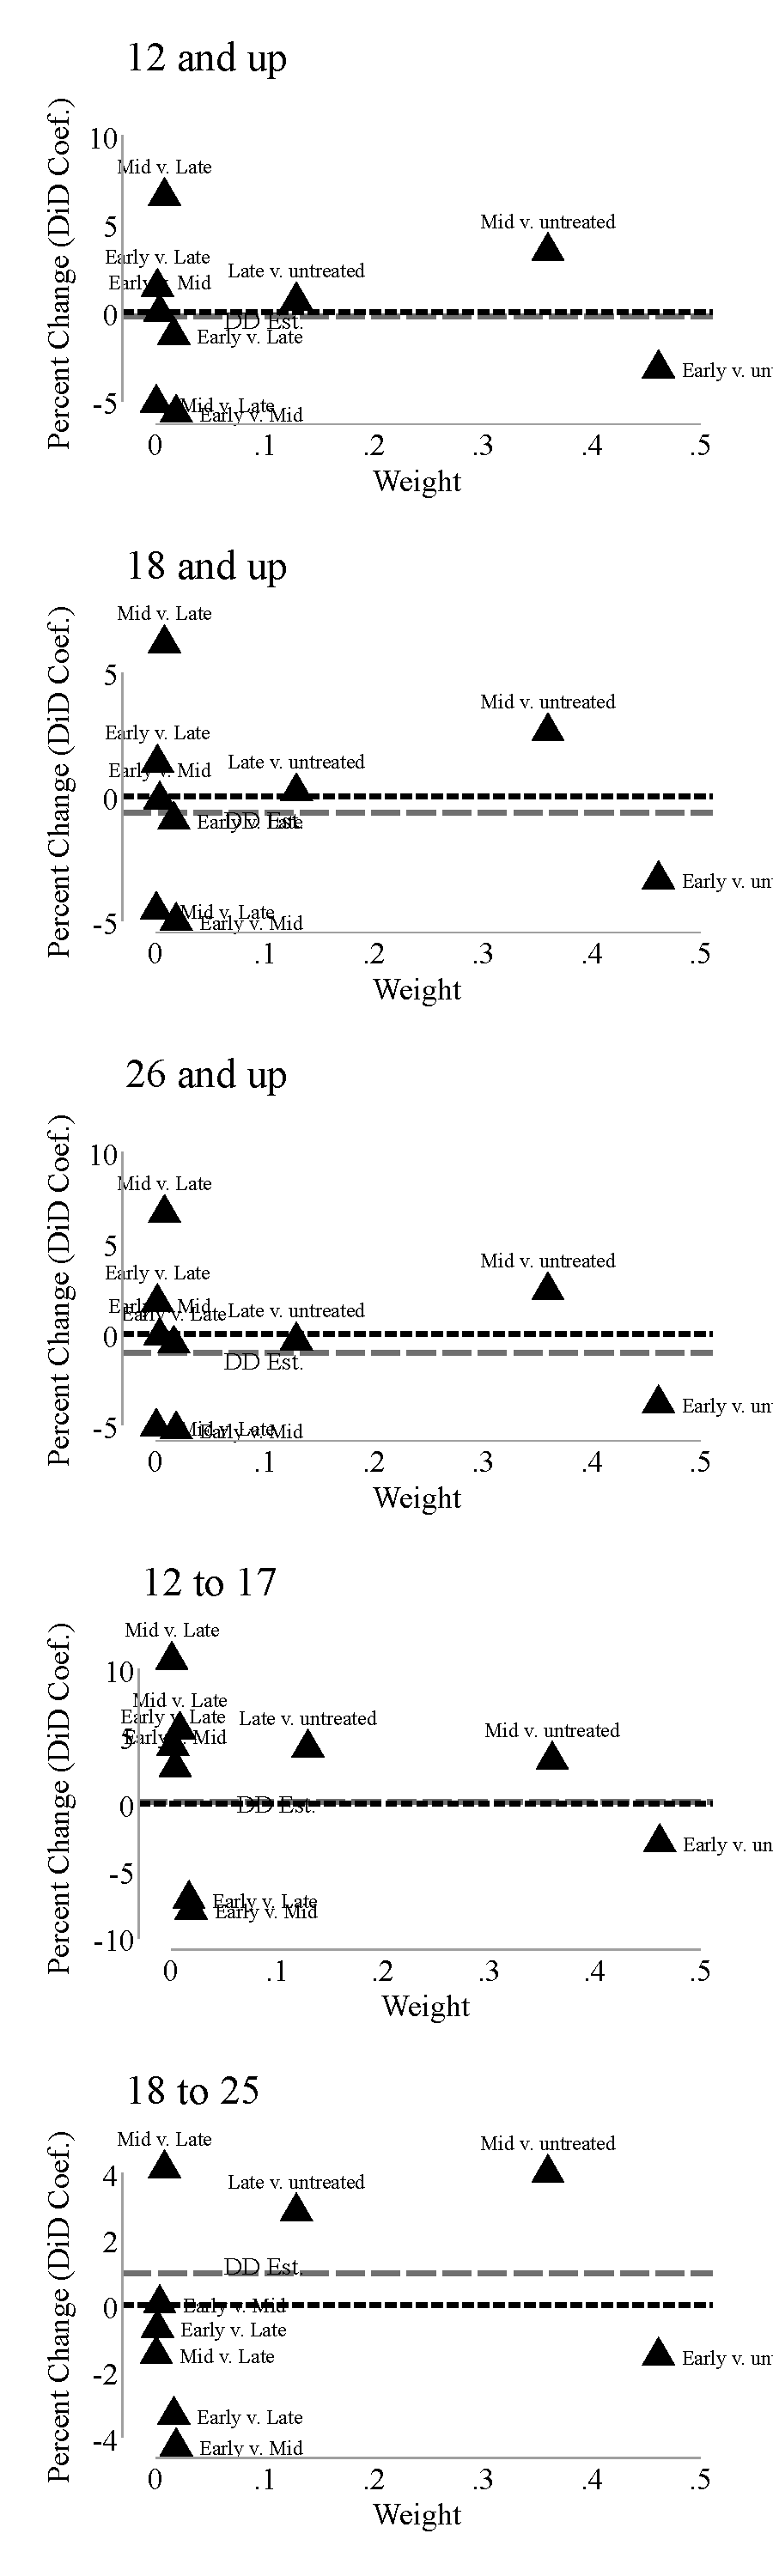
\includegraphics[width=\linewidth]{../output/plots/bacon_weights_ln_alc_use_30.pdf}
    \label{fig:bacon_lead_lag_alc_30}
  \end{subfigure}
  \hfill %%
  \begin{subfigure}[b]{0.32\columnwidth}
      \caption{\scriptsize{Tobacco use in past 30 days}}
    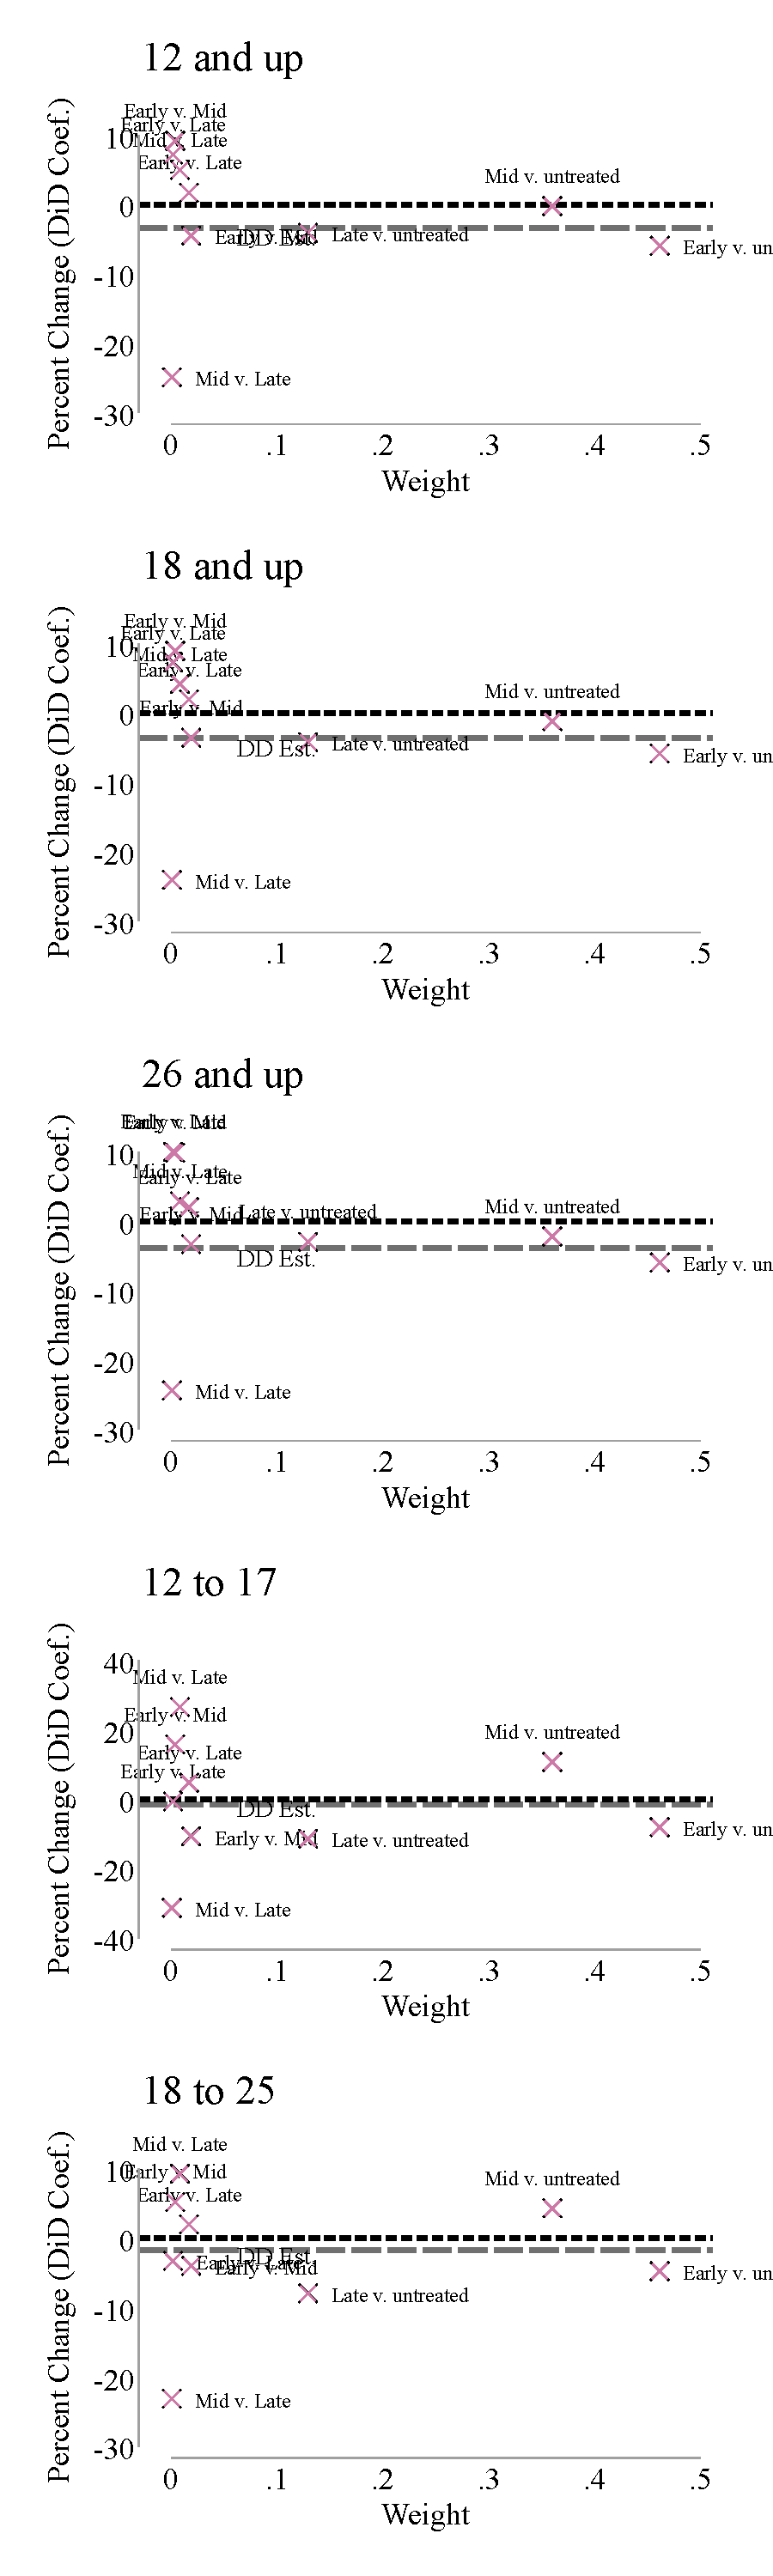
\includegraphics[width=\linewidth]{../output/plots/bacon_weights_ln_tob_use_30.pdf}
    \label{fig:bacon_lead_lag_tob_30}
  \end{subfigure}
   \hfill %%
  \begin{subfigure}[b]{0.32\columnwidth}
    \caption{\scriptsize{Cocaine use in past year}}
    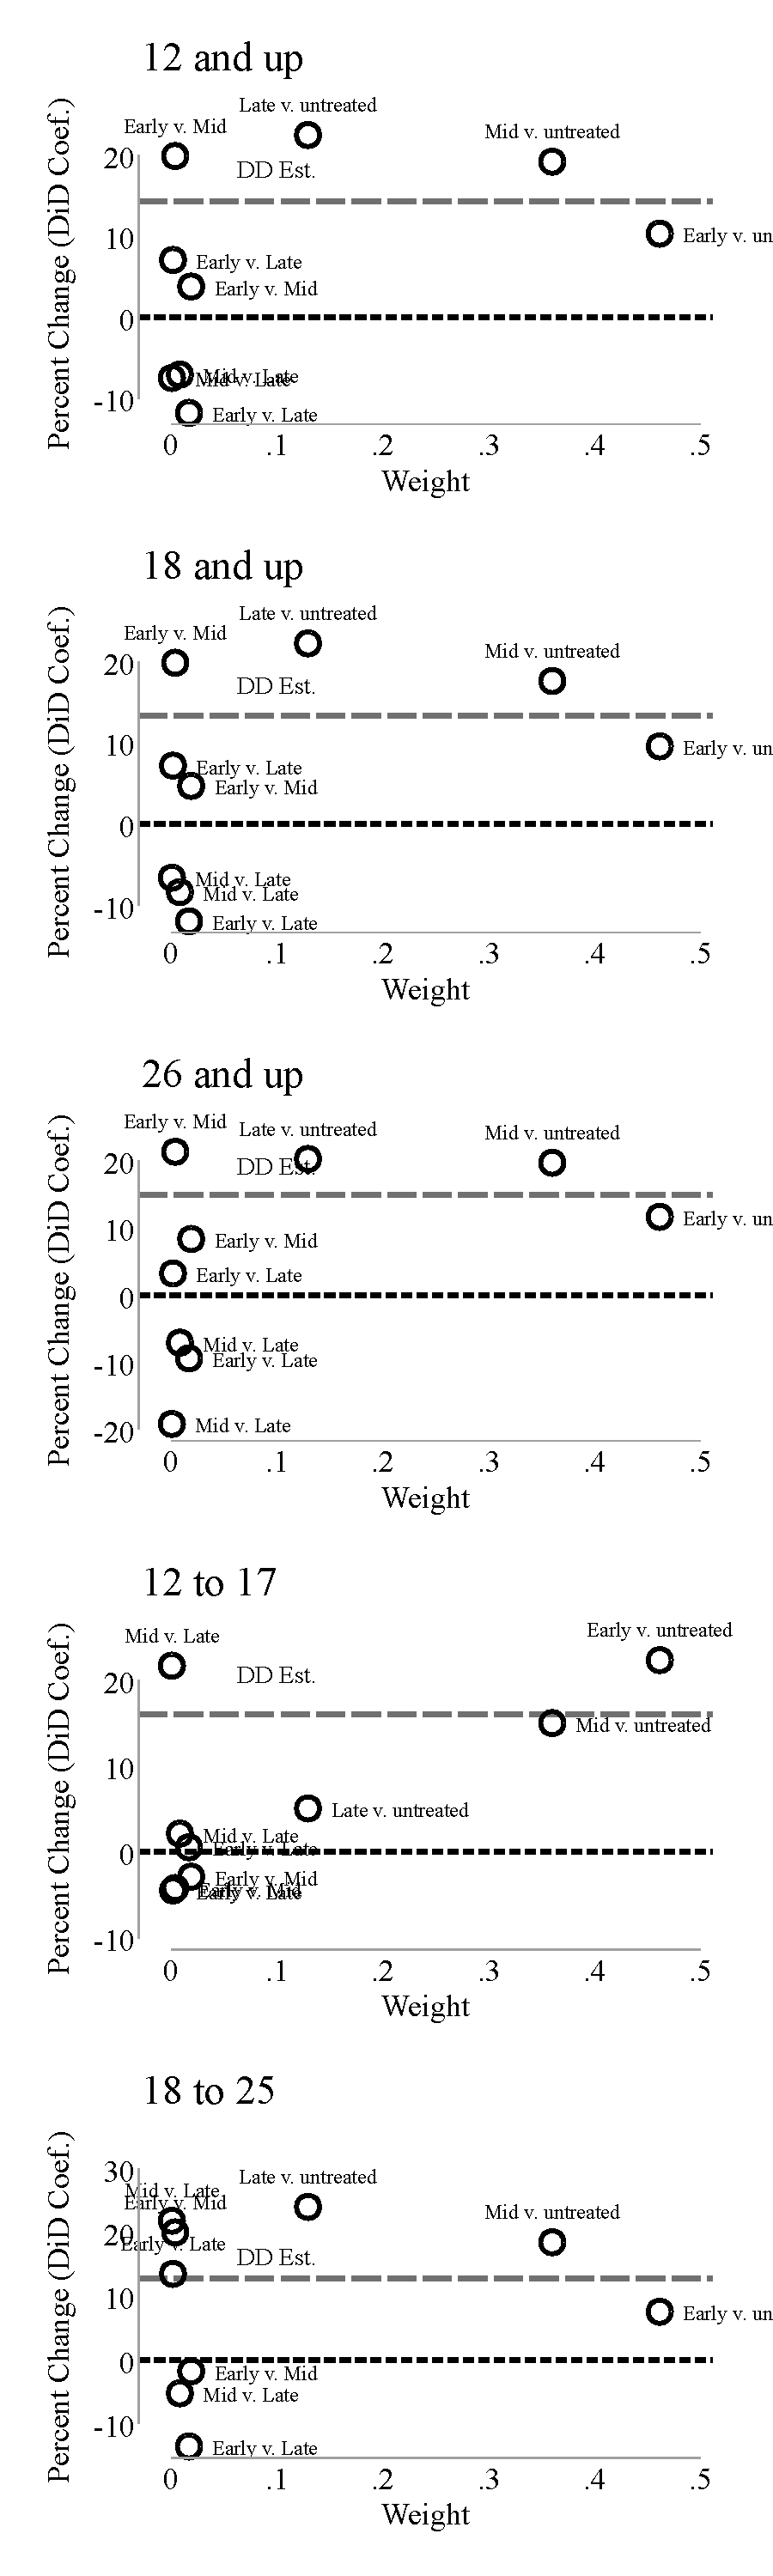
\includegraphics[width=\linewidth]{../output/plots/bacon_weights_ln_coke_use_365.pdf}
    \label{fig:bacon_lead_lag_coke_365}
  \end{subfigure}
  \label{fig:bacon_lead_lag_oth}
 \begin{justify}
                {\footnotesize \vspace{-.5cm}
                    \emph{Note:} 
    Weights are constructed as in Goodman-Bacon (2018).
    Each point plots the 2x2 DID coefficient from a comparison of the two groups in the label against the weight given to that group in the combined DID regression.
    The gray dashed line denotes the average DID treatment effect estimate and the black dashed line is at zero.
    The average DID treatment effect estimate reported here is the average of the y-values for each point weighted by their respective x-values.
    For ease of exposition, the regressions used to obtain these estimates include only state and year fixed-effects and do not control for other policy or control variables.
    We use the model coefficients to compute $\% \Delta \approx 100\times \left[exp(\beta_1)-1\right]$, which is the percent change in the prevalence of drug use generated a given policy change.     
    There are four total groups, one untreated group and three treated AKA timing groups (i.e. states that eventually adopt recreational marijuana laws).
    A timing group is characterized by the policy adoption year:
    early includes Colorado and Washington (panel wave 2012/2013);
    mid includes Alaska, Oregon, and Washington DC (panel wave 2015/2016);
    and late includes California and Massachusetts (panel wave 2016/2017).
\par}
            \end{justify}
  \end{minipage}
\end{figure}


\begin{figure}[h]
    \caption{The impact of recreational marijuana legalization on other drug use by age group.}
        \begin{minipage}{\linewidth}
      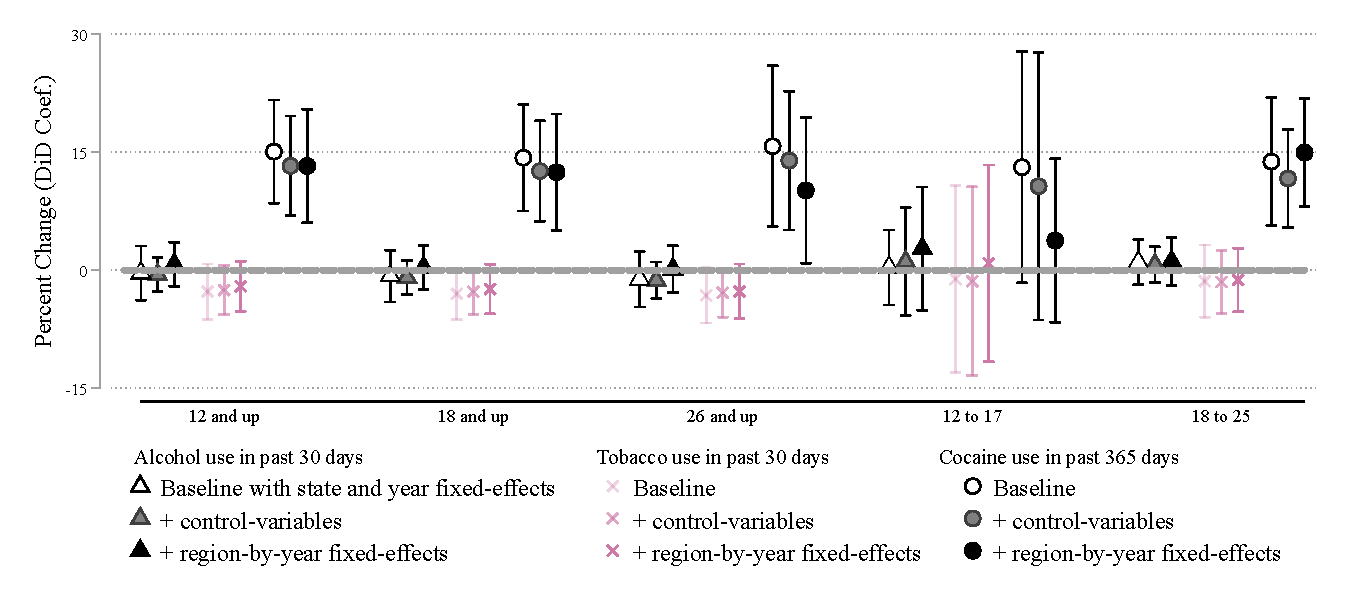
\includegraphics[width=\linewidth]{../output/plots/aux_figure_for_paper_robust_part_a.pdf}
       \label{fig:aux_coef_plot}
        \vspace{-1cm}
     \begin{justify}
                {\footnotesize
                    \emph{Note:} 
        Color and shape are associated with the dependent variable, while shade is associated with the specification.
       The baseline specification includes only indicators for the status of medical marijuana, medical dispensary, and recreational marijuana legalization in each state and year along with state and year fixed-effects.
       The baseline does not include control variables.
       Control variables are the unemployment rate, median income, \% white, \% male. 
       The dependent variable is the natural log of the prevalence of drug use in state $s$ in period $t$ for a specified age group and type of drug. We use the model coefficients to compute $\% \Delta \approx 100\times \left[exp(\beta_1)-1\right]$, which is the percent change in the prevalence of drug use generated a given policy change.  We use a cluster robust variance matrix that allows for dependency at the state level to estimate standard errors for the coefficients, and we use the delta method to compute standard errors and associated 95\% confidence intervals that are reported in brackets. 
                \par}
            \end{justify}
    \end{minipage}
    \end{figure}

\begin{figure}
    \caption{Leads and lags of impact of recreational marijuana legalization on substance use by age group.}
            \begin{minipage}{.9\linewidth}
  \begin{subfigure}[b]{0.32\columnwidth}
    \caption{Alcohol use in past 30 days}
    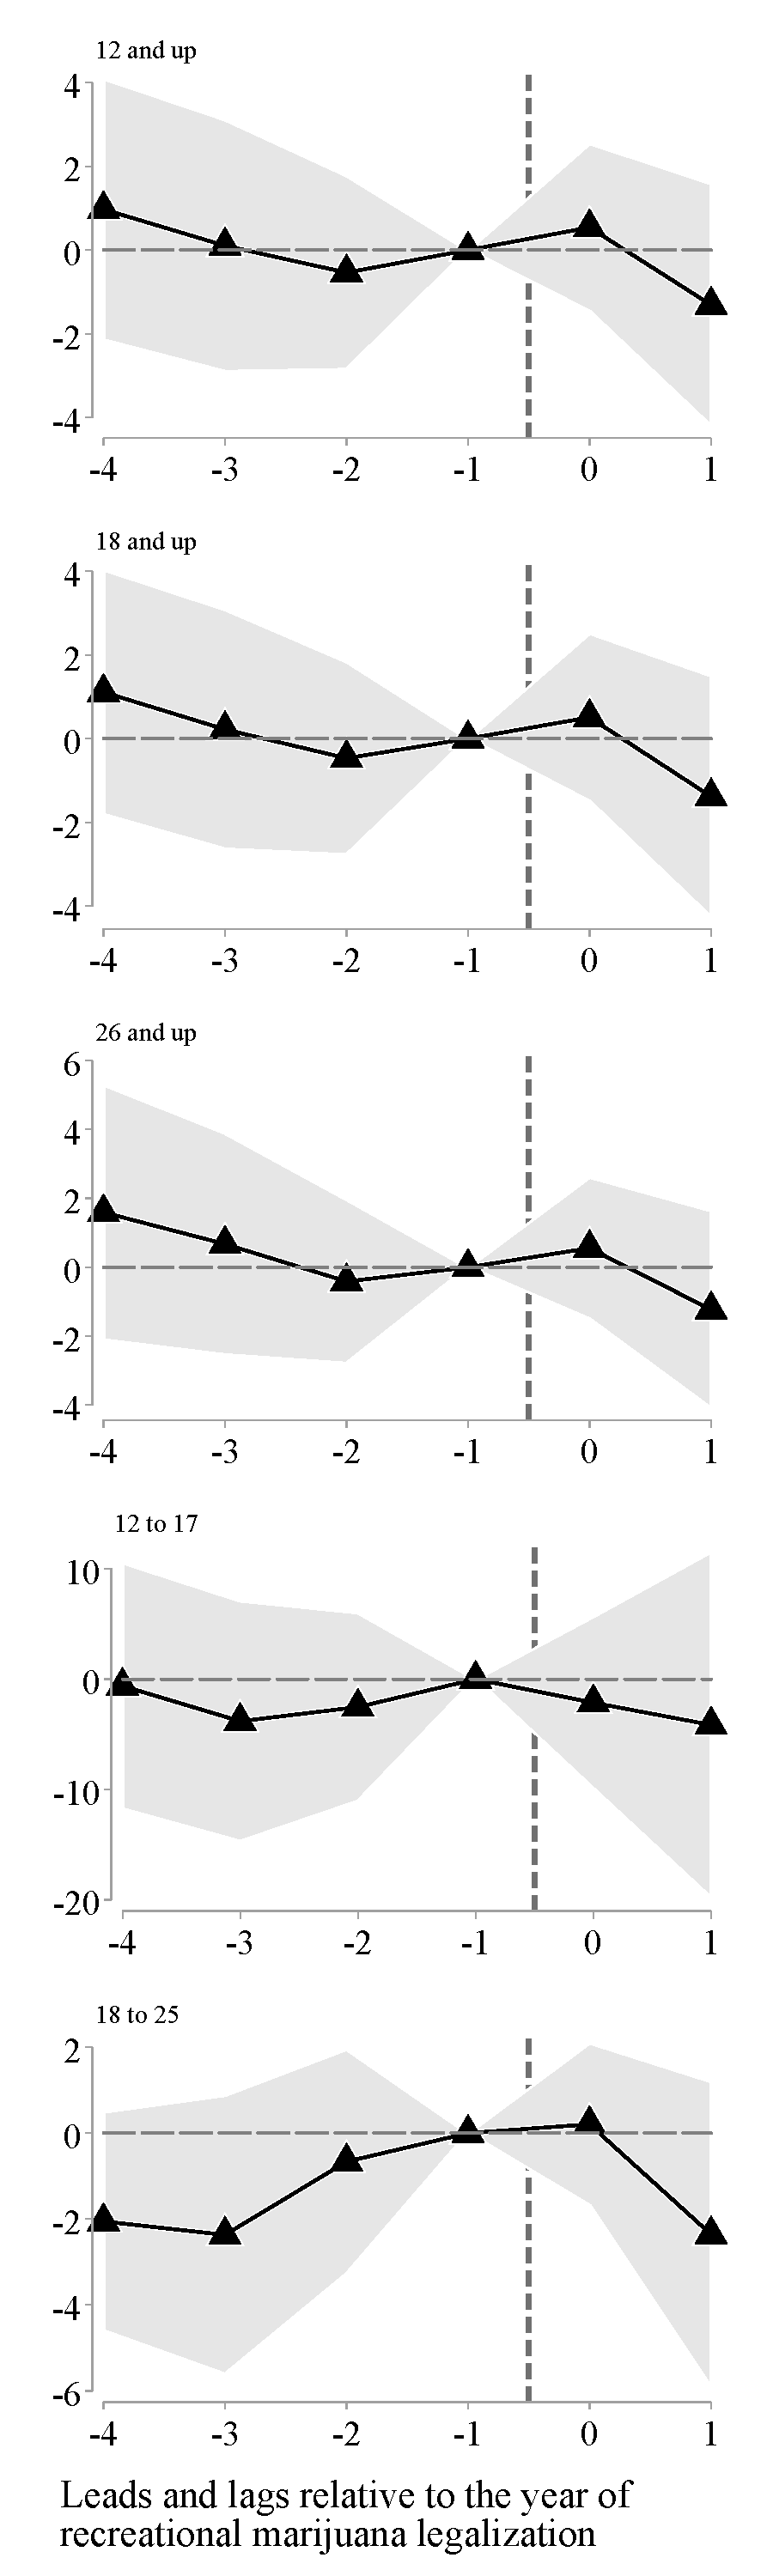
\includegraphics[width=\linewidth]{../output/plots/event-study-estimates-ln-alc_use_30.pdf}
    \label{fig:lead_lag_alc_30}
  \end{subfigure}
  \hfill %%
  \begin{subfigure}[b]{0.32\columnwidth}
      \caption{Tobacco use in past 30 days}
    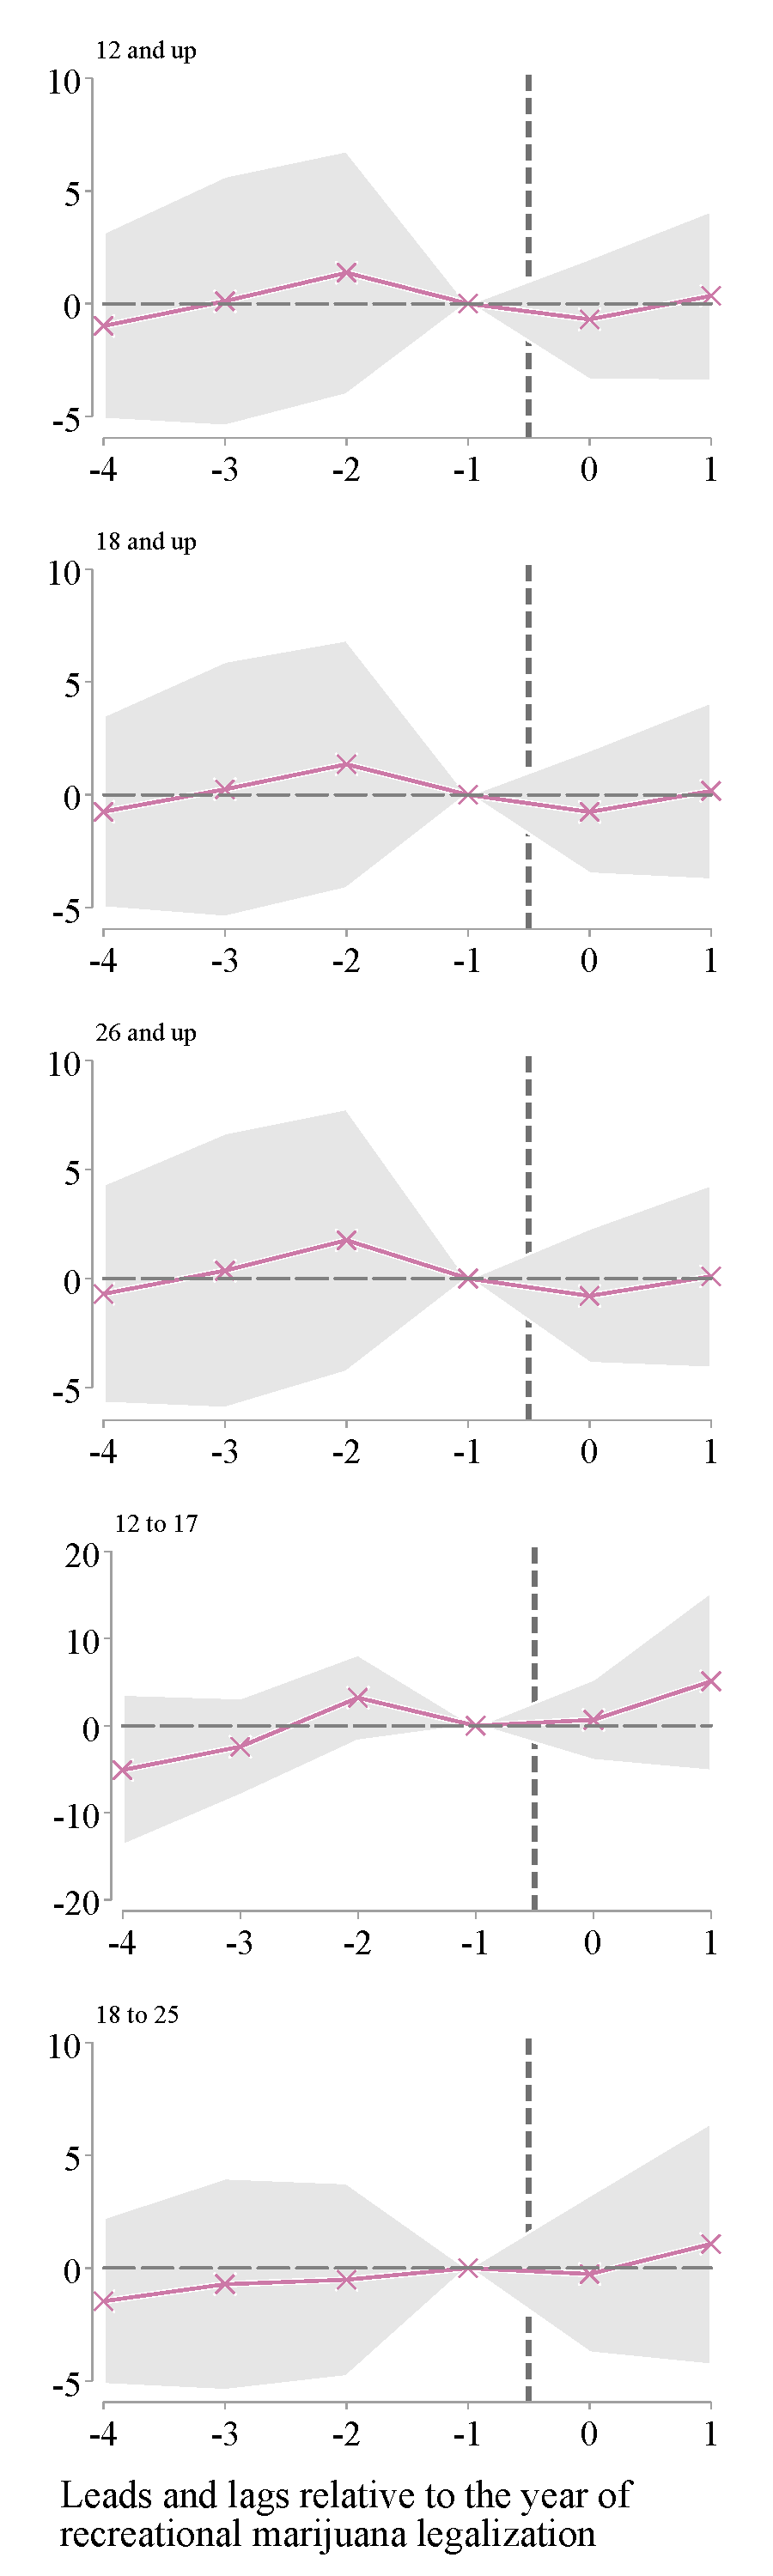
\includegraphics[width=\linewidth]{../output/plots/event-study-estimates-ln-tob_use_30.pdf}
    \label{fig:lead_lag_tob_30}
  \end{subfigure}
   \hfill %%
  \begin{subfigure}[b]{0.32\columnwidth}
    \caption{Cocaine use in past year}
    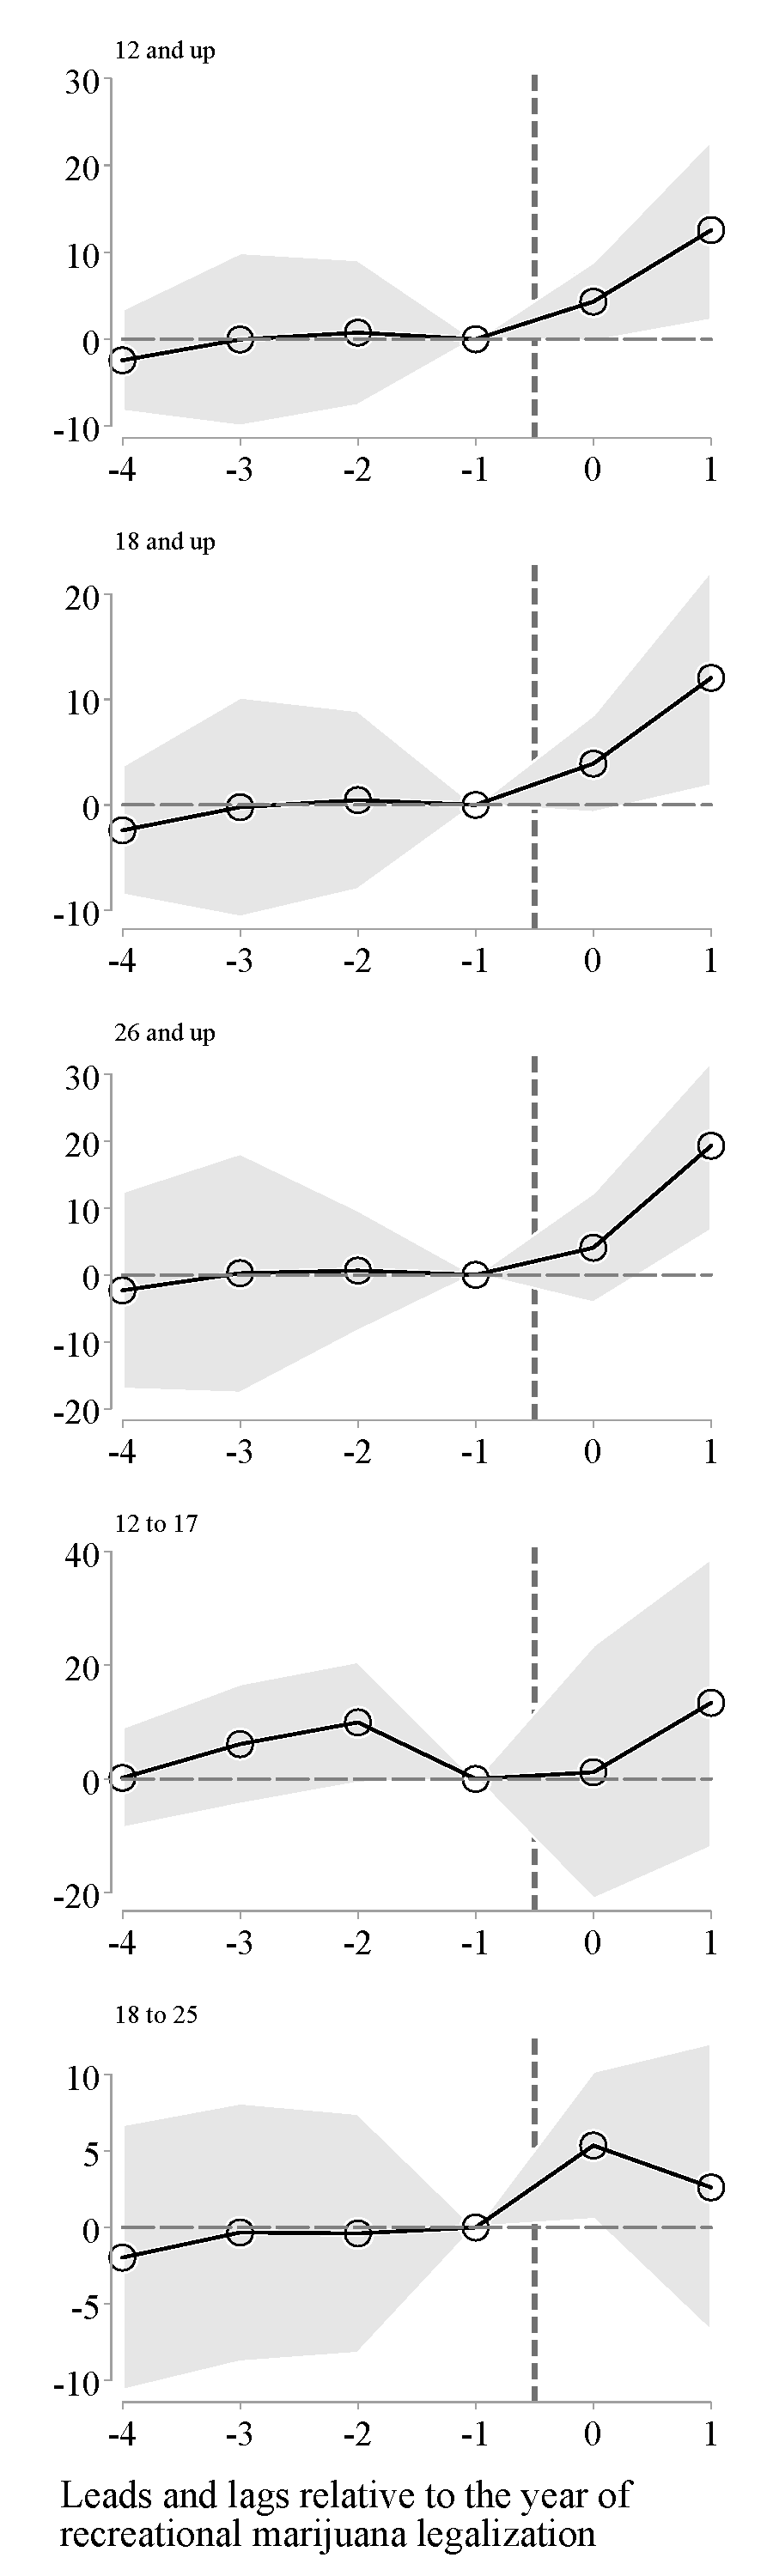
\includegraphics[width=\linewidth]{../output/plots/event-study-estimates-ln-coke_use_365.pdf}
    \label{fig:unbalanced_lead_lag_coke_365}
  \end{subfigure}
        \label{fig:unbalanced_lead_lag_other}
 \begin{justify}
                {\footnotesize
                    \emph{Note:} 
            The dependent variable is the natural log of the prevalence of drug use in state $s$ in period $t$ for a specified age group and type of drug. We use the model coefficients to compute $\% \Delta \approx 100\times \left[exp(\beta_1)-1\right]$, which is the percent change in the prevalence of drug use generated a given policy change.  We use a cluster robust variance matrix that allows for dependency at the state level to estimate standard errors for the coefficients, and we use the delta method to compute standard errors for the transformed coefficients and associated 95\% confidence intervals, which are reported by the shaded area. The standard error refers to the standard error of the combined effect. The regressions adjust for unemployment rate, median income, \% white, and \% male. 
                \par}
            \end{justify}
       \end{minipage}
\end{figure}



\FloatBarrier




    % Recreational marijuana and other substance use
      \begin{table}[ht]\centering
          \begin{adjustbox}{width=.85\textwidth}
          \centering
            \begin{threeparttable}
              \caption{The impact of recreational marijuana on substance use by age group and frequency of use.}
              \estauto{../output/tables/other_use_full_table_add_rm_disp.tex}{6}{S[table-format=1.2,table-column-width=20mm]}
              \label{tab:other_use_add_rm_disp}
             \Fignote{
                 * p $<$ 0.1, ** p $<$ 0.05, *** p $<$ 0.01.
The dependent variable is the natural log of the prevalence of drug use in state $s$ in period $t$ for a specified age group and type of drug. We use the model coefficients to compute $\% \Delta \approx 100\times \left[exp(\beta_1)-1\right]$, which is the percent change in the prevalence of drug use generated a given policy change.  We use a cluster robust variance matrix that allows for dependency at the state level to estimate standard errors for the coefficients, and we use the delta method to compute standard errors for the transformed coefficients. The standard errors are shown in parenthesis. The results that include dispensaries report the combined estimated treatment effect of legalization and  of dispensaries opening.  We compute the combined effect by adding the estimated coefficients on the binary indicator for medical (recreational) marijuana  and the binary indicator for medical (recreational) dispensary and then using the transformation above to compute the percentage effect. The standard error refers to the standard error of the combined effect. The regressions adjust for unemployment rate, median income, \% white, and \% male. }          %\Figsource{We good the data from here.}
            % \Starnote
            \end{threeparttable}
           \end{adjustbox}
        \end{table}

%------------------------------------------%
%     Event Studies
%------------------------------------------%
\begin{figure}[H]
    \caption{Event study estimates of effect recreational marijuana legalization on the \% of drug tests that are positive for THC.}
    \begin{minipage}{\linewidth}
      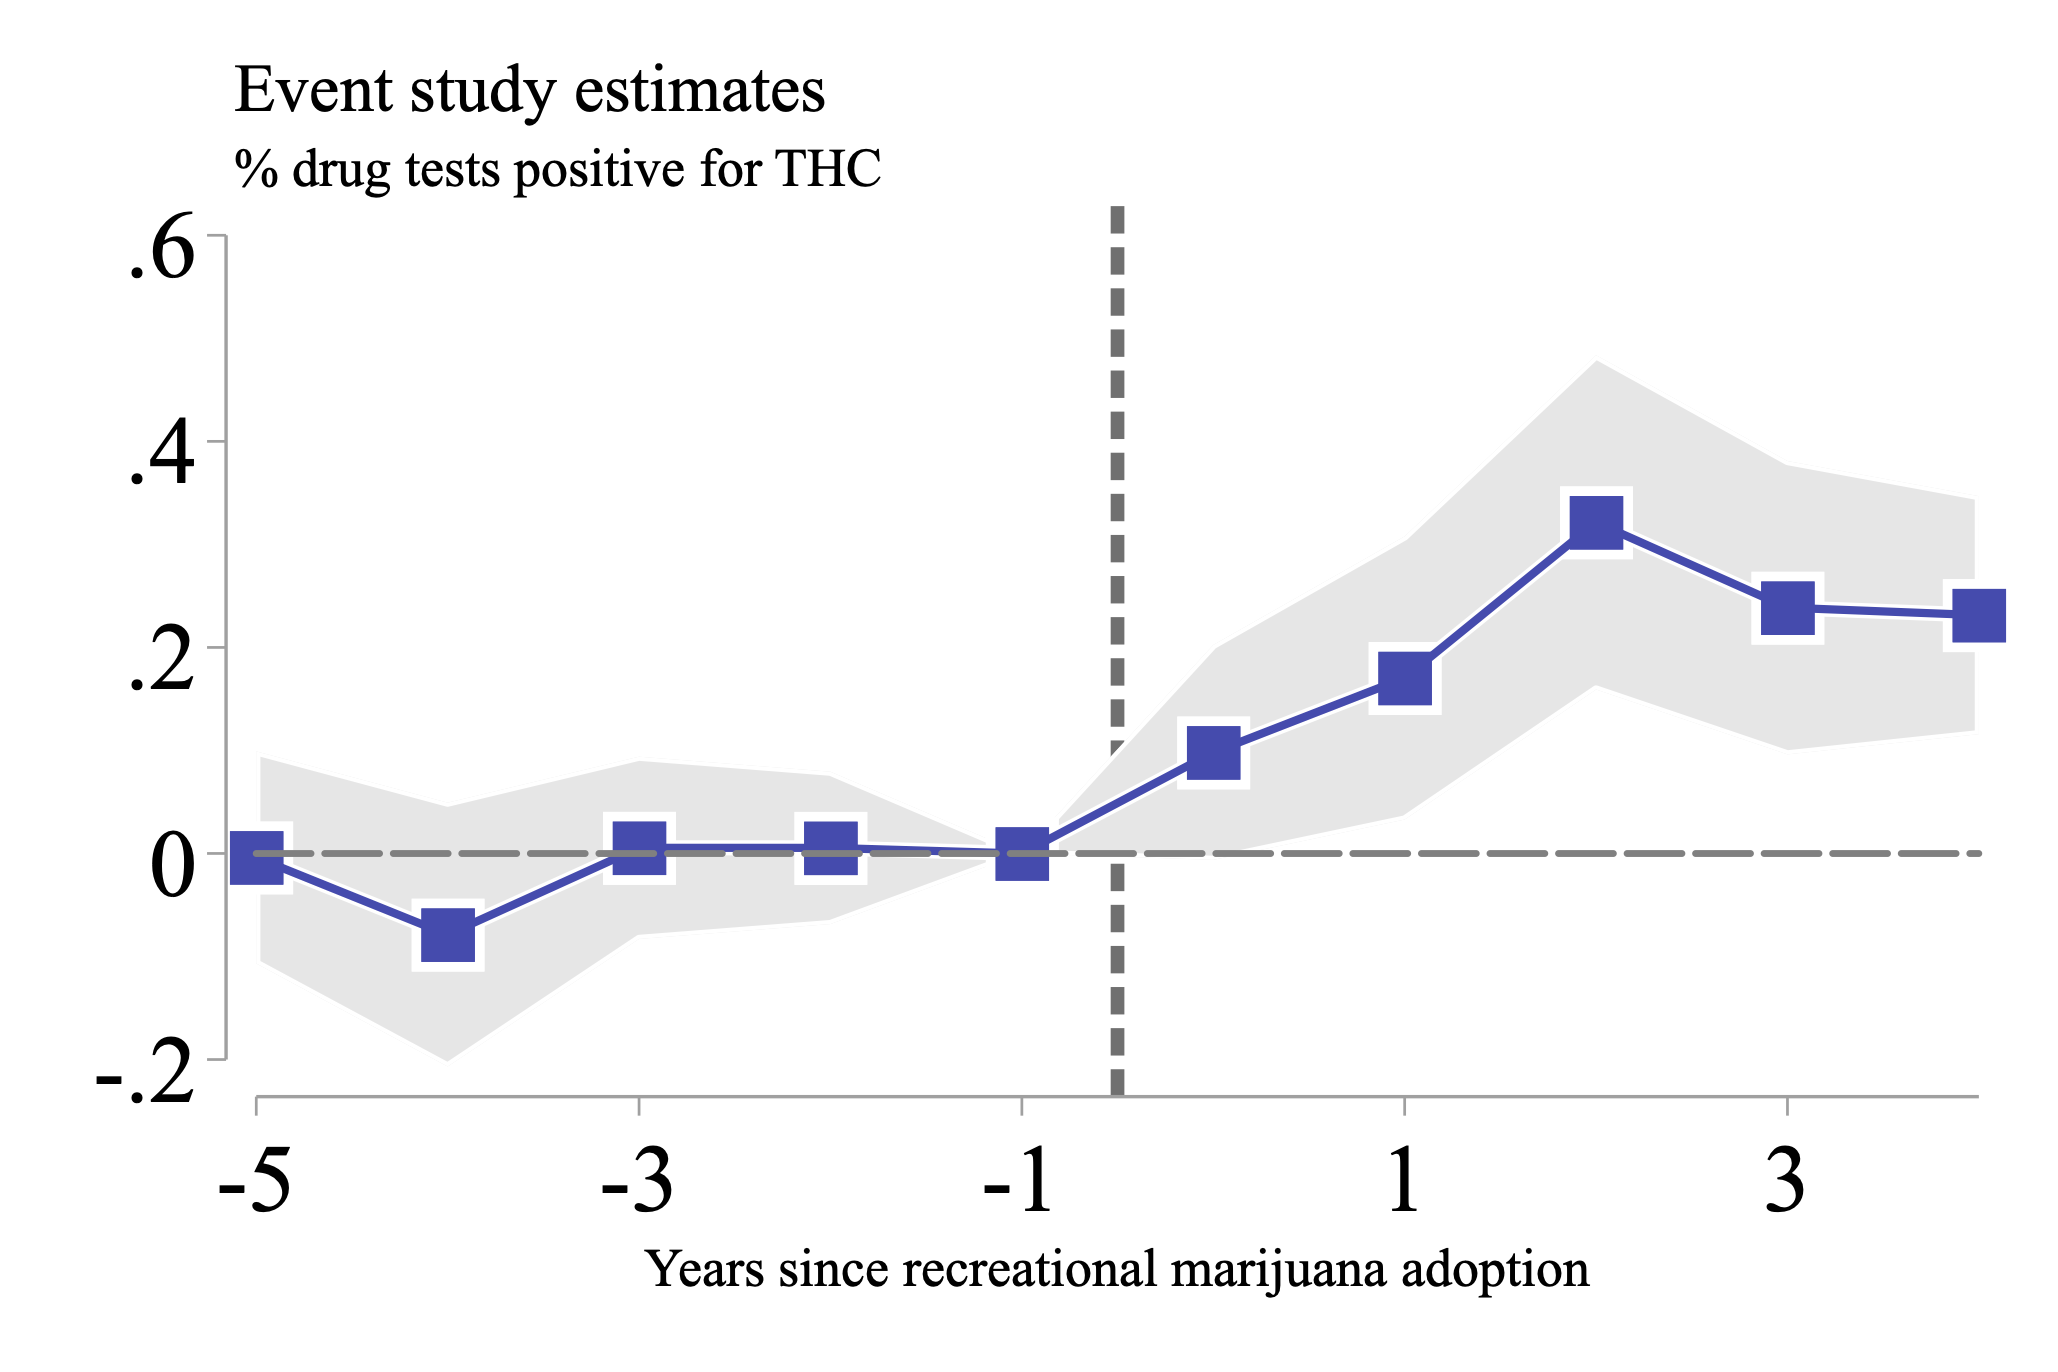
\includegraphics[width=\linewidth]{../output/plots/event-study-percent_test_positive_for_thc.png}
       \label{fig:event-study-drug-tests}
        \vspace{-1cm}
              \begin{justify}
                {\footnotesize
                    \emph{Note:} 
             This figure shows the effect of recreational marijuana legalisation on the percent (\%[0-100]) of drug tests that detect THC (the primary psychoactive compound in marijuana). 
       The x-axis denotes years since recreational adoption, with negative values indicating years prior to adoption. 
       The specification includes indicators for the status of medical marijuana and medical dispensaries being open in each state and year, along with state and region-by-year fixed-effects.
       We use the model coefficients to compute $\% \Delta \approx 100\times \left[exp(\beta_1)-1\right]$, which is the percent change in the prevalence of drug use generated a given policy change.  We use a cluster robust variance matrix that allows for dependency at the state level to estimate standard errors for the coefficients, and we use the delta method to compute standard errors for the transformed coefficients and associated 95\% confidence intervals, which are reported by the shaded area.
                \par}
            \end{justify}
       \end{minipage}
    \end{figure}
\FloatBarrier

\subsection{Robustness Checks and Sensitivity Analysis}
\label{sec:robust_a}

We conducted supplementary analysis to probe the sensitivity of our results to key threats to validity. 
We start by examining whether the statistical significance of our results is sensitive to different approaches to conducting statistical inference that rely on weaker assumptions about the error structure of the model. 
Then we give a short summary of a series of robustness checks we used to examine concerns about the structure of the NSDUH SAE data, alternative coding of state law changes, different model specifications, and tests for compositional change. Overall, the supplementary analysis supports our main conclusions. 

\subsubsection{Statistical Inference}
\label{sec:inference}
The cluster robust variance matrix we use throughout the paper may produce standard errors that are too small with a finite number of states and a relatively small number of treated states. To assess the sensitivity of our conclusions to this concern, we estimate sampling distributions under the null hypothesis of no effect using two procedures based on randomization inference. Both approaches work by randomly assigning placebo marijuana policy changes to randomly chosen state-year cells. One approach uses a flexible law generating process and the other uses a restrictive law generating process.

In the flexible procedure, we conduct 500 simulations. In each simulation, we randomly chose integers between 1 and 50 to determine how many states will experience each of the three regulatory changes (recreational, medical, dispensary-medical). Then we randomly select the treated states, randomly assign each of the treated states an adoption year for each variable, and create the three pseudo law variables. Finally, we regress observed outcomes on the placebo marijuana regulation variables, covariates, state fixed-effects, and region-by-year fixed-effects.

The flexible procedure allows a broader range of possible configurations of policy changes that actually occurred in our data and this could lead to a narrower sampling distribution than a law generating process that more closely mimics the collection of treatment changes in our study. Accordingly, we also considered a more restrictive randomization procedure in which we permute the distribution of regulatory variables within census regions. Specifically, in each of the 500 simulations, we swap each state’s full policy time series (recreational, medical,  dispensary-medical, and dispensary-recreational) with the policy time series of another state in the same census region. Then we estimate our preferred two-way fixed effects regression. 
In both simulations, we used the empirical distribution of the 500 placebo law coefficient estimates to test the null hypothesis that each law had no effect on the drug use outcomes in our study. Specifically, we compute p values from the randomization distribution using:

\begin{align*}
p= \frac{1}{500} \sum_{k=1}^{500} 1(abs(\widehat{\theta(k)}) \geq abs((\widehat{\theta_{Data}}))
\end{align*}

In the formula, $\widehat{\theta_{Data}}$ is a parameter estimate from our actual data, and $\widehat{\theta(k)}$  is the corresponding parameter estimate from the $k^{th}$ simulation. $E[\widehat{\theta(k)}]=0$ across the simulations, but some simulations will generate a large $\widehat{\theta(k)}$ just by chance. The p-value measures the proportion of simulations with a point estimates at least as large in absolute value as the one observed in our data. The randomization inference procedures allow for observations that are dependent within state, but they are less prone to over rejecting the null hypothesis than cluster robust standard errors. Table~\ref{tab:ri_p_values} shows that the randomization inference p-values are not meaningfully different from the p-values obtained from tests based on clustered standard errors.

\subsubsection{Sample Construction, Weighting, Data Coding}

\paragraph{Comparing NSDUH to other survey data on marijuana use}
%Measurement in NSDUH vs YRBS
One concern with our results is that the passage of recreational marijuana laws may have made people more willing to report their marijuana use in survey settings, even when privacy may be in doubt. This concern may be particularly salient for adolescent respondents in the NSDUH who could be answering sensitive questions while their parents are nearby. To shed some light on this alternative interpretation, we examined data on adolsecent marijuana use from the nationally representative version of the YRBS. Since the YRBS is collected in schools using paper-and-pencil self-administered questionnaires, it may be less subject to concerns about bystander effects. The orange lines in figure \ref{fig:yrbs_nsudh_monthly} shows the difference in prevalence of 12-17 year olds who report using marijuana in the past month (top panel) and the ever (bottom panel) from 2003 to 2017. The green line shows the fraction of 12-17 year olds in the United States who are living in states that have implemented recreational marijuana laws. Over the period covered in the graph, the fraction of adolescents living in recreational marijuana states grew from 0 to more than 20 percent. In contrast, the gap between the NSDUH and the YRBS is quite stable over the entire period. This graph cannot tell us which survey provides a more accurate measure of adolescent marijuana use. But it does suggest that the reporting differences between the two surveys has not changed much in response to changes in state marijuana laws. 


%No panel overlap.
\paragraph{Drop overlapping years}
The NSDUH SAE data we use in the main analysis is based on two-year waves of data. This means that adjacent waves of the NSDUH SAE share some overlapping data. Table~\ref{tab:mj_full_table_add_rm_disp_drop_odd} shows results from models in which we drop every other year from the NSDUH SAE data. This ensures that there is no overlap in data from one year to the next. Despite losing almost 50\% of the data, our main results are unchanged, indicating that the overlapping structure of the NSDUH SAE data is not driving our results. 

%Aggressive treatment. 
\paragraph{Use alternative treatment dates}
Appendix Tables~\ref{tab:mj_use_aggressive} and~\ref{tab:other_use_aggressive} show that our main results are robust to using an aggressive timing variable outlined in section~\ref{sec:data_laws}. With this timing definition the combined effect of recreational marijuana legalization and recreational dispensaries is at least twice as large as the effect of recreational marijuana legalization without dispensaries for almost every age group and measure of use. The results support our claim that the conservative coding procedure used in our main analysis produces estimates that are -- if anything -- biased towards zero.

% Pop weights
\paragraph{Use population weights}
Tables~\ref{tab:mj_use_pop_weights} and~\ref{tab:other_use_pop_weights} shows that the results are very similar when we weight the observations by state population size; however, the effects of recreational laws on cocaine use are not statistically significant in this specification.

%Untransformed
\paragraph{Level instead of log-transform}
Tables~\ref{tab:mj_use_pop_mean} and~\ref{tab:other_use_pop_mean} show that our main results are robust to using the untransformed mean of drug use rather than the natural log transform.

\subsubsection{Model Robustness Checks}

%Balance Test
\paragraph{Covariate balance}
Under the common trends assumption, the policy changes should not be associated with changes in the composition of the states over time. Table~\ref{tab:covariate_balance_table} shows a fixed effects version of a balance table that follows \citet{Pei2019} by assessing whether the policy changes predict changes in time varying covariates after adjusting for fixed effects. The outcome variables in these balance tests regressions are time varying covariates that are not included in our main results. This test helps evaluate the identification assumption that the variation in our independent variables of interest is unrelated to omitted variables after conditioning our preferred set of fixed effects. After controlling for state and region-by-year fixed effects, we find no clear evidence that the adoption of recreational marijuana induces changes in or is related to total population, \% Hispanic, \% aged 0 to 14, \% aged 15 to 24,  \% aged 25 to 44,  \% aged 45 to 64, \% 65+,  violent crime rate, or property crime rate. We find some evidence that recreational marijuana adopting states see a dip in the \% of the  black population, however this difference is only significant at the 10\% level and is small in magnitude. Taken together the results from the balancing supports the common trends assumption.

%Examine pop distribution
\paragraph{Does legalization affect population distribution?}
The common trends assumption might fail if states that adopted recreational marijuana laws were experiencing compositional changes that might affect levels of drug use. Table~\ref{tab:mj_and_pop} shows estimated coefficients from regressions of the natural log of state sub-population sizes on the marijuana regulation variables and fixed effects. In models that do not include census region-by-year fixed effects (top panel), the adoption of recreational laws and medical laws are associated with small changes in the size of some sub-populations. However, the magnitude and significance of these effects decline to almost zero when census region-by-year effects are included in the model. This may indicate that the regions where recreational and medical marijuana law adopting states are located had changing population patterns, but the adopting states did not have differential population changes relative to their respective regions. This pattern of results is why we prefer effect estimates from models that allow for regions specific time trends. 

%Limit to similar pre-period mean
\paragraph{Limit control states based on similar substance use}
To assess concerns that recreational marijuana states may have had higher marijuana use even before the policy changes and that initially high marijuana use might be associated with faster growth rates, we constructed comparison groups that were matched on pre-treatment outcome levels for each outcome and age group. Specifically, we restricted the control states to those that had pre-treatment mean outcomes within 1.5 standard deviations of the pre-treatment mean in the recreational marijuana states. The results are in Table~\ref{tab:mj_use_only_good_pretrends} (marijuana) and~\ref{tab:other_only_good_pretrendss} (other drugs). Tables~\ref{tab:only_good_pretrends_list_mj} and~\ref{tab:only_good_pretrends_list_oth} list the states included in each restricted regression. The estimated effects of recreational marijuana laws from these matched comparison group models are very similar to the results from our main analysis. The estimated effects of medical marijuana tend to show somewhat larger effects in the matched comparison group models than in our main analysis.

%common trends weak vs strong
\paragraph{Alternative sets of time varying fixed effects}
In Appendix Tables~\ref{tab:mj_use_no_region_fe} to~\ref{tab:oth_use_division-by-year}, we estimate regulatory effects from models that impose both stronger and weaker forms of the common trends assumption. Tables~\ref{tab:mj_use_no_region_fe} and~\ref{tab:other_use_no_region_fe} report estimates from models that include only state and year fixed effects, which assume a common trend in all states rather than allowing trends that vary across census regions. Tables~\ref{tab:mj_use_no_region_fe_no_control} and~\ref{tab:other_use_no_region_fe_no_control} report estimates from models that include only state and year fixed effects and do not include control variables. 
We also explored using census division-by-year fixed effects instead or census region-by-year fixed effects. 
There are nine census divisions (compared to 4 census regions) and the states within a given division may be more comparable to one another than states within a region. 
For example, the Northeast census region is composed of nine states and two divisions: the New England division contains Connecticut, Maine, Massachusetts, New Hampshire, Rhode Island, and Vermont; and the Middle Atlantic division contains New Jersey, New York, and Pennsylvania. 
A nice feature of the census division-by-year fixed effects (and more broadly the census region-by-year fixed effects) is that they will capture, and net away, any spill over effects of one state's recreational marijuana policy on nearby states, which has been observed in prior work \citep{HanenSpillovers2020}. 
We present these results  in Tables~\ref{tab:mj_use_division-by-year} and~\ref{tab:oth_use_division-by-year}. 
The estimated effects of recreational marijuana and medical marijuana legalization on marijuana use are virtually unchanged across these different specifications. 

%------------------------------------------%
%    Randomization inference
%------------------------------------------%

\begin{table}[ht]\centering
	\begin{adjustbox}{width=.9\textwidth}
		\centering
		 \caption{Randomization inference based p-values for impact of recreational marijuana on use of each substance by age group.}
		   \label{fig:randomization_table}
		\centering
		\begin{tabular}{llccc}
			\toprule
			{Substance}&{Age Group}&{\shortstack{Regression\\ based p-value}}&{\shortstack{Fully randomized\\ p-value}}&{\shortstack{Randomized within\\ region p-value}} \tabularnewline
\midrule \addlinespace[\belowrulesep]
\emph{Marijuana use in the past 365 days}&12 to 17&$<$ 0.001&0.028&0.056 \tabularnewline
&18 to 25&0.002&0.018&0.000 \tabularnewline
&12 and up&$<$ 0.001&0.016&0.000 \tabularnewline
&18 and up&$<$ 0.001&0.016&0.000 \tabularnewline
&26 and up&$<$ 0.001&0.018&0.002 \tabularnewline
\addlinespace[1.5ex]\emph{Marijuana use in the past 30 days}&12 to 17&0.002&0.028&0.026 \tabularnewline
&18 to 25&0.024&0.020&0.030 \tabularnewline
&12 and up&$<$ 0.001&0.016&0.000 \tabularnewline
&18 and up&$<$ 0.001&0.016&0.000 \tabularnewline
&26 and up&$<$ 0.001&0.016&0.000 \tabularnewline
\addlinespace[1.5ex]\emph{New marijuana initiates in the past two years}&12 to 17&$<$ 0.001&0.024&0.046 \tabularnewline
&18 to 25&0.047&0.018&0.018 \tabularnewline
&12 and up&0.001&0.022&0.006 \tabularnewline
&18 and up&0.007&0.020&0.004 \tabularnewline
&26 and up&$<$ 0.001&0.022&0.018 \tabularnewline
\addlinespace[1.5ex]\emph{Alcohol use in the past 30 days}&12 to 17&0.427&0.280&0.616 \tabularnewline
&18 to 25&0.581&0.352&0.724 \tabularnewline
&12 and up&0.458&0.282&0.520 \tabularnewline
&18 and up&0.572&0.416&0.632 \tabularnewline
&26 and up&0.660&0.540&0.740 \tabularnewline
\addlinespace[1.5ex]\emph{Tobacco use in the past 30 days}&12 to 17&0.908&0.758&0.920 \tabularnewline
&18 to 25&0.574&0.346&0.592 \tabularnewline
&12 and up&0.048&0.056&0.132 \tabularnewline
&18 and up&0.027&0.044&0.100 \tabularnewline
&26 and up&0.011&0.034&0.086 \tabularnewline
\addlinespace[1.5ex]\emph{Cocaine use in the past 365 days}&12 to 17&0.210&0.162&0.394 \tabularnewline
&18 to 25&0.006&0.046&0.040 \tabularnewline
&12 and up&0.033&0.042&0.092 \tabularnewline
&18 and up&0.048&0.046&0.124 \tabularnewline
&26 and up&0.224&0.060&0.268 \tabularnewline


			\bottomrule 
		\end{tabular}
		\label{tab:ri_p_values}
	\end{adjustbox}
	{\footnotesize
	\begin{justify}
	    \emph{Note}:
		The regression based p-values report p-values from the results reported in Tables~\ref{tab:mj_use_add_rm_disp} and~\ref{tab:other_use_add_rm_disp}.
		Section~\ref{sec:inference} discusses the two randomization inference procedures used to calculate the fully randomized and randomization within census region p-values.
		The p-value from each procedure reports the proportion of times that the absolute value of the actual treatment effect is smaller than the absolute value of a treatment effect from 500 regressions were treatment was randomly assigned.
		In the fully randomized procedure, we randomly assign all treatment status and start dates for each state and policy (medical, recreational, dispensaries).
		For each of the 500 draws, we randomly chose integers between 1 and 50 to determine how many states will experience each of the three regulatory changes (recreational, medical, dispensary-medical, dispensary-recreational).
		Then we randomly select the pseudo-treated states, randomly assign each of the pseudo-treated states an adoption year for each variable, and create the three pseudo law variables.
		In the randomized within-region procedure, we randomly swap the entire policy path (status of recreational, medical, dispensary-medical, and dispensary-recreational in each year) of each state with another in the same census region.
	\end{justify}
	}
\end{table}
\begin{figure}[H]
    \caption{The reporting gap between the NSDUH and YRBSS does not change as more states legalize recreational marijuana.}
    \begin{minipage}{.55\linewidth}
      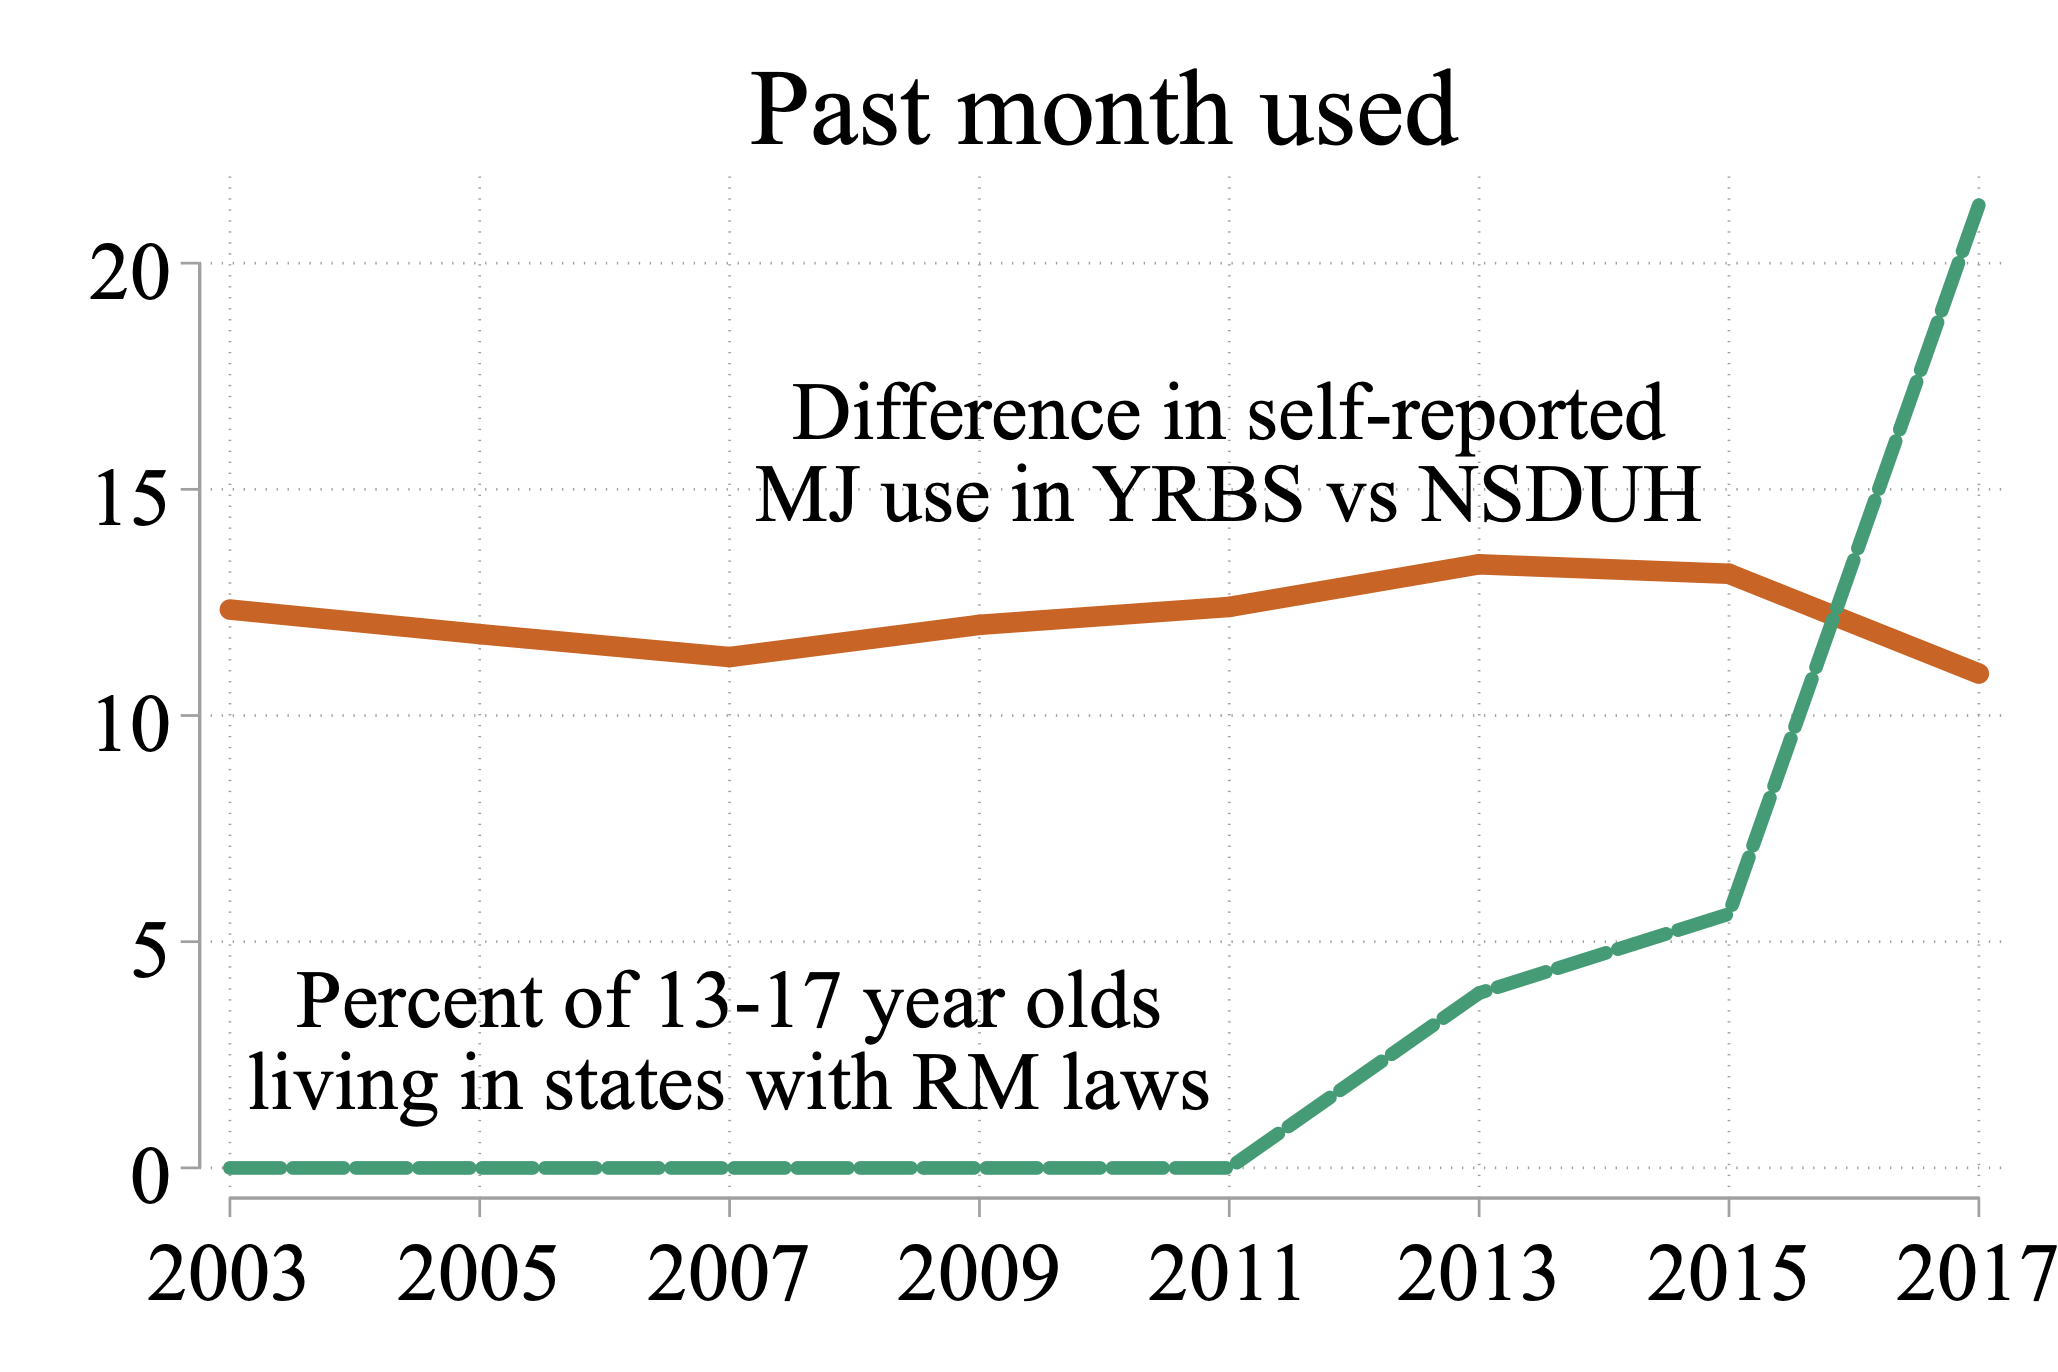
\includegraphics[width=\linewidth]{../output/plots/marijuana_30_pop.png}
       \label{fig:yrbs_nsudh_monthly}
      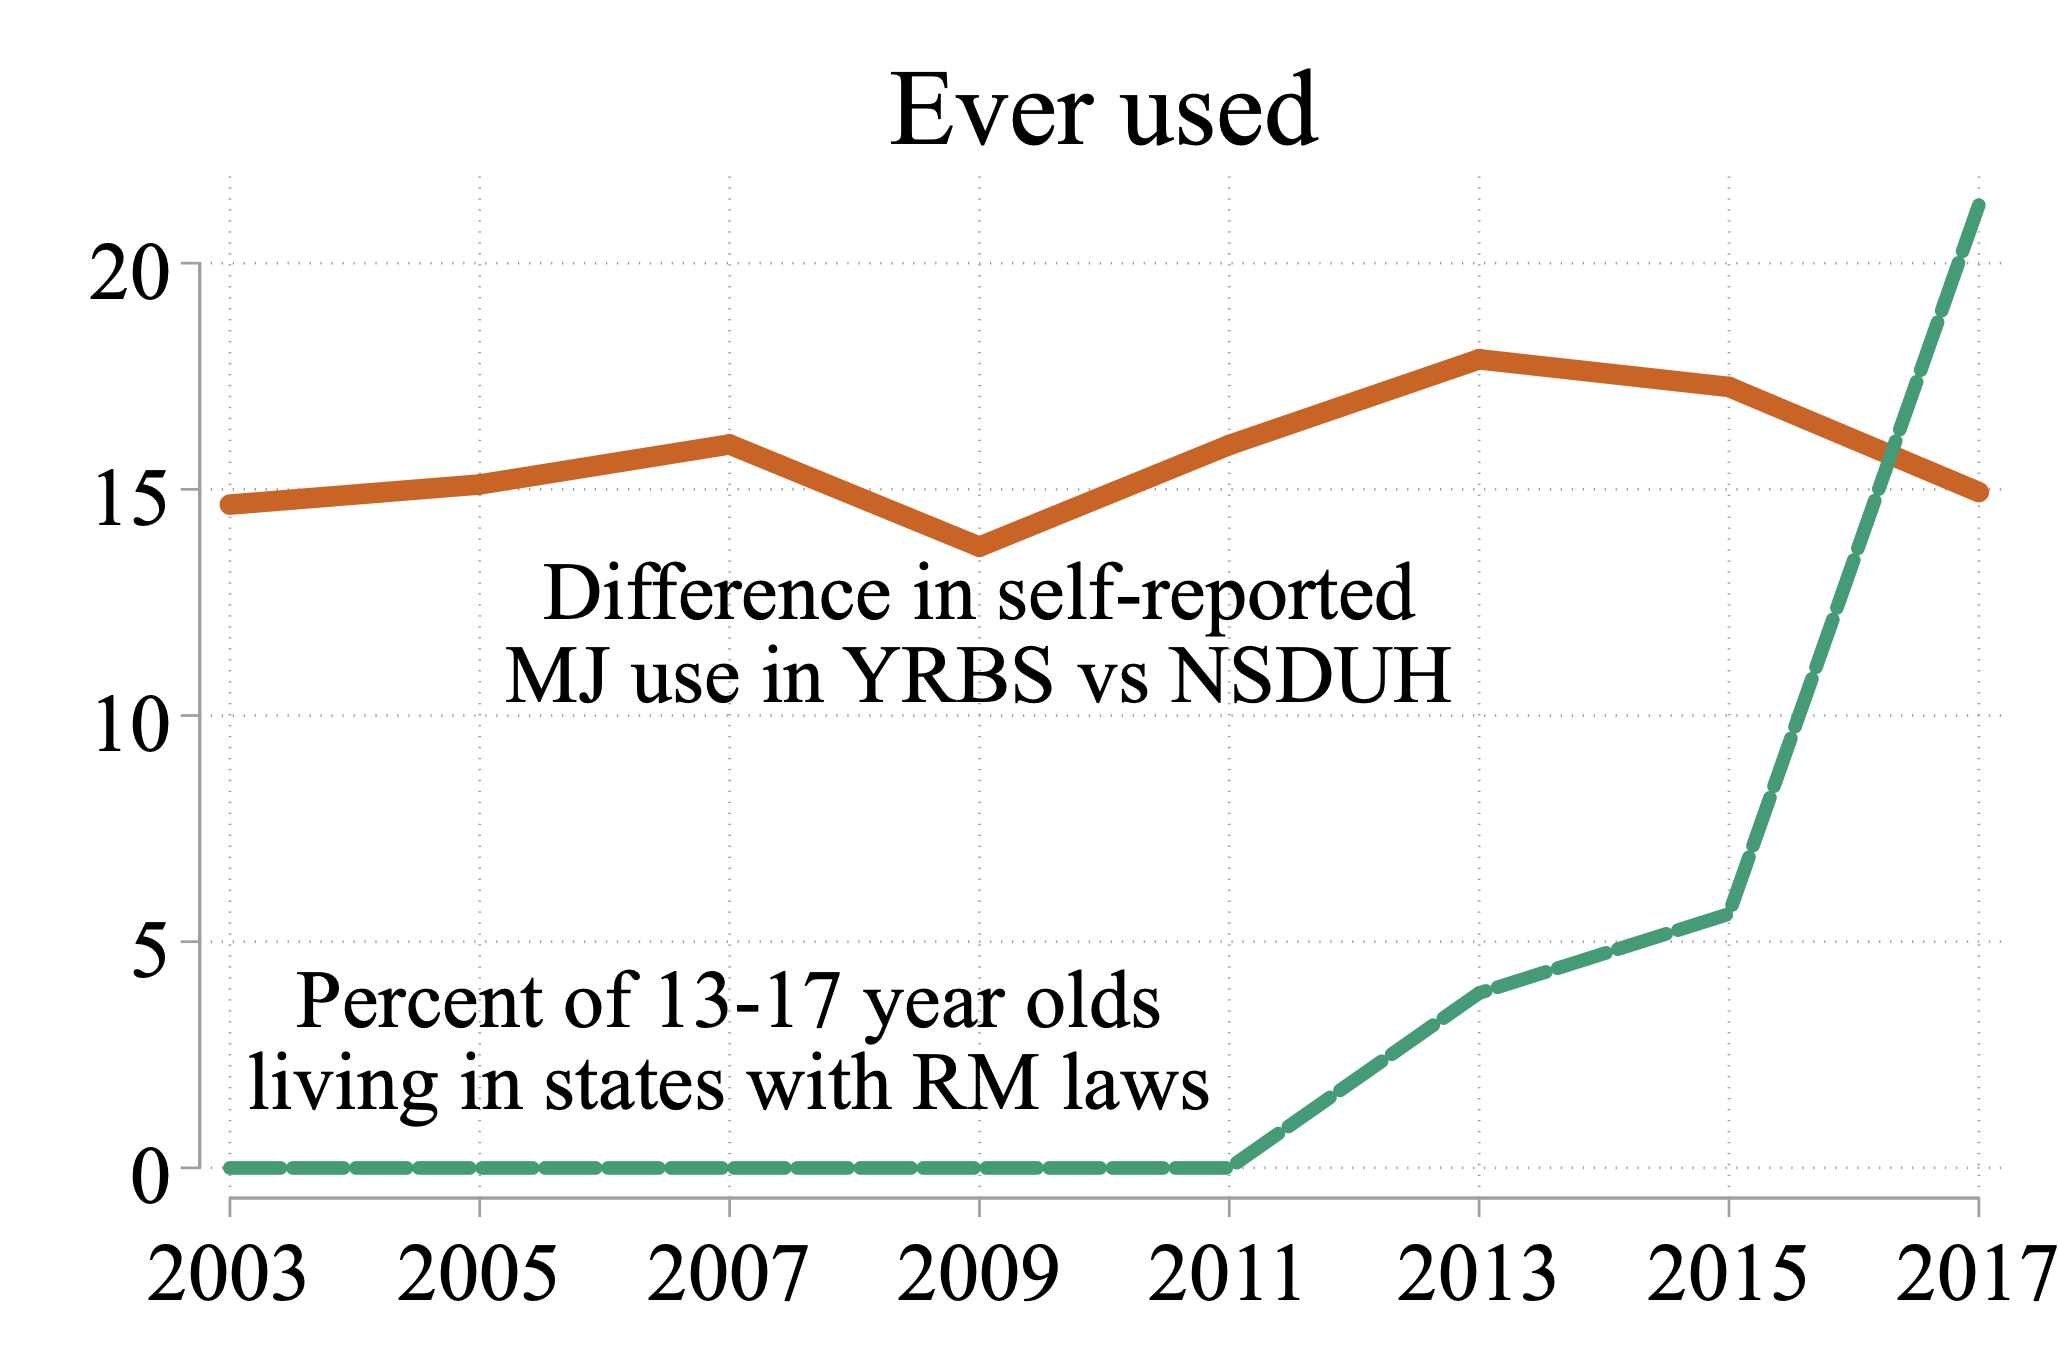
\includegraphics[width=\linewidth]{../output/plots/marijuana_ever_pop.png}
       \label{fig:yrbs_nsudh_ever}
       \begin{justify}
                {\footnotesize
                    \emph{Note:} 
        The solid orange line shows the difference in reported marijuana use for those aged 13 to 17 between the NSDUH and YRBS surveys. 
        Differences for reported past 30 day marijuana use are displayed on top, while differences in reported ever having used marijuana are displayed on the bottom. 
        The dashed green line reports the percent of 13-17 year olds that live in states with recreational marijuana laws in each year. This percent increases as more states adopt recreational marijuana policies.
        The difference between self-reported marijuana use was calculated using the national YRBSS files and the national NSDUH files. Due to the ways that these files categorize ages, only adolescents from age 13-17 were included. The percent of adolescents aged 13-17 living in states with recreational laws was calculated using SEER data.
                \par}
            \end{justify}
        \end{minipage}
        \label{fig:nsduh-v-yrbs}
    \end{figure}


   % Recreational marijuana and marijuana use
\begin{table}[ht]\centering
    \begin{adjustbox}{width=.85\textwidth}
        \centering
        \begin{threeparttable}
            \caption{The impact of recreational marijuana on marijuana use by age group and frequency of use: Dropping every other year so there is no  overlap in panel years.}
            \estauto{../output/tables/mj_full_table_add_rm_disp_drop_odd.tex}{6}{S[table-format=1.2,table-column-width=20mm]}
            \label{tab:mj_full_table_add_rm_disp_drop_odd}
            \Fignote{
            Here we exclude every other year from our data so there is no overlap in the years included in the analysis.
            For example, our main specification would include data from the 2001-2002, 2002-2003, and 2003-2004 NSDUH SAE.
            In this specification we only include the 2001-2002 and 2003-2004 data.
             * p $<$ 0.1, ** p $<$ 0.05, *** p $<$ 0.01.
            The dependent variable is the natural log of the prevalence of drug use in state $s$ in period $t$ for a specified age group and type of drug. We use the model coefficients to compute $\% \Delta \approx 100\times \left[exp(\beta_1)-1\right]$, which is the percent change in the prevalence of drug use generated a given policy change.  We use a cluster robust variance matrix that allows for dependency at the state level to estimate standard errors for the coefficients, and we use the delta method to compute standard errors for the transformed coefficients. The standard errors are shown in parenthesis. The results that include dispensaries report the combined estimated treatment effect of legalization and  of dispensaries opening.  We compute the combined effect by adding the estimated coefficients on the binary indicator for medical (recreational) marijuana  and the binary indicator for medical (recreational) dispensary and then using the transformation above to compute the percentage effect. The standard error refers to the standard error of the combined effect. The regressions adjust for unemployment rate, median income, \% white, and \% male. 
               }
        \end{threeparttable}
    \end{adjustbox}
\end{table}


% Recreational marijuana and marijuana use
\begin{table}[ht]\centering
    \begin{adjustbox}{width=.8\textwidth}
    \centering
      \begin{threeparttable}
        \caption{The impact of recreational marijuana on marijuana use by age group and frequency of use: with an aggressive treatment variable.}
        \estauto{../output/tables/mj_full_table_add_rm_disp_agr.tex}{6}{S[table-format=1.2,table-column-width=20mm]}
        \label{tab:mj_use_aggressive}
         \Fignote{
                 * p $<$ 0.1, ** p $<$ 0.05, *** p $<$ 0.01.
               Aggressive treatment means that we consider any panel wave with a treated year to be treated.
               This differs from Table~\ref{tab:mj_use_add_rm_disp}, where treatment is considered to be the first panel wave where both years are treated.
               For example, if a dispenary opened in 2014, Table~\ref{tab:mj_use_add_rm_disp} would consider the wave 2013-2014 to be untreated and the wave 2014-2015 to be treated.
               In this Table with aggressive treatment both of the waves would be considered treated.
               The dependent variable is the natural log of the prevalence of drug use in state $s$ in period $t$ for a specified age group and type of drug. We use the model coefficients to compute $\% \Delta \approx 100\times \left[exp(\beta_1)-1\right]$, which is the percent change in the prevalence of drug use generated a given policy change.  We use a cluster robust variance matrix that allows for dependency at the state level to estimate standard errors for the coefficients, and we use the delta method to compute standard errors for the transformed coefficients. The standard errors are shown in parenthesis. The results that include dispensaries report the combined estimated treatment effect of legalization and  of dispensaries opening.  We compute the combined effect by adding the estimated coefficients on the binary indicator for medical (recreational) marijuana  and the binary indicator for medical (recreational) dispensary and then using the transformation above to compute the percentage effect. The standard error refers to the standard error of the combined effect. The regressions adjust for unemployment rate, median income, \% white, and \% male. }
      \end{threeparttable}
     \end{adjustbox}
\end{table}

% Recreational marijuana and other substance use
\begin{table}[ht]\centering
  \begin{adjustbox}{width=.8\textwidth}
  \centering
    \begin{threeparttable}
      \caption{The impact of recreational marijuana on substance use by age group and frequency of use: with an aggressive treatment variable.}
      \estauto{../output/tables/other_use_full_table_add_rm_disp_agr.tex}{6}{S[table-format=1.2,table-column-width=20mm]}
      \label{tab:other_use_aggressive}
     \Fignote{
         * p $<$ 0.1, ** p $<$ 0.05, *** p $<$ 0.01.
                   Aggressive treatment means that we consider any panel wave with a treated year to be treated.
                   This differs from Table~\ref{tab:other_use_add_rm_disp}, where treatment is considered to be the first panel wave where both years are treated.
                   For example, if a dispenary opened in 2014, Table~\ref{tab:other_use_add_rm_disp} would consider the wave 2013-2014 to be untreated and the wave 2014-2015 to be treated.
                   In this Table with aggressive treatment both of the waves would be considered treated.
                   The dependent variable is the natural log of the prevalence of drug use in state $s$ in period $t$ for a specified age group and type of drug. We use the model coefficients to compute $\% \Delta \approx 100\times \left[exp(\beta_1)-1\right]$, which is the percent change in the prevalence of drug use generated a given policy change.  We use a cluster robust variance matrix that allows for dependency at the state level to estimate standard errors for the coefficients, and we use the delta method to compute standard errors for the transformed coefficients. The standard errors are shown in parenthesis. The results that include dispensaries report the combined estimated treatment effect of legalization and  of dispensaries opening.  We compute the combined effect by adding the estimated coefficients on the binary indicator for medical (recreational) marijuana  and the binary indicator for medical (recreational) dispensary and then using the transformation above to compute the percentage effect. The standard error refers to the standard error of the combined effect. The regressions adjust for unemployment rate, median income, \% white, and \% male. }   
    \end{threeparttable}
   \end{adjustbox}
\end{table}
 
%------------------------------------------%
%                Table A
%------------------------------------------%
% Recreational marijuana and marijuana use
\begin{table}[ht]\centering
    \begin{adjustbox}{width=.9\textwidth}
    \centering
      \begin{threeparttable}
        \caption{The impact of recreational marijuana on marijuana use by age group and frequency of use: with population weights.}
        \estauto{../output/tables/mj_full_table_pop_weights.tex}{6}{S[table-format=1.2,table-column-width=20mm]}
        \label{tab:mj_use_pop_weights}
         \Fignote{
        * p $<$ 0.1, ** p $<$ 0.05, *** p $<$ 0.01.
        Regressions are weighted by total state population.
        The dependent variable is the natural log of the prevalence of drug use in state $s$ in period $t$ for a specified age group and type of drug. We use the model coefficients to compute $\% \Delta \approx 100\times \left[exp(\beta_1)-1\right]$, which is the percent change in the prevalence of drug use generated a given policy change.  We use a cluster robust variance matrix that allows for dependency at the state level to estimate standard errors for the coefficients, and we use the delta method to compute standard errors for the transformed coefficients. The standard errors are shown in parenthesis. The results that include dispensaries report the combined estimated treatment effect of legalization and  of dispensaries opening.  We compute the combined effect by adding the estimated coefficients on the binary indicator for medical (recreational) marijuana  and the binary indicator for medical (recreational) dispensary and then using the transformation above to compute the percentage effect. The standard error refers to the standard error of the combined effect. The regressions adjust for unemployment rate, median income, \% white, and \% male.}
      \end{threeparttable}
     \end{adjustbox}
\end{table}

%------------------------------------------%
%                Table A
%------------------------------------------%
% Recreational marijuana and other substance use
\begin{table}[ht]\centering
    \begin{adjustbox}{width=.85\textwidth}
    \centering
      \begin{threeparttable}
        \caption{The impact of recreational marijuana on substance use by age group and frequency of use: with population weights.}
        \estauto{../output/tables/other_use_full_table_pop_weights.tex}{6}{S[table-format=1.2,table-column-width=20mm]}
        \label{tab:other_use_pop_weights}
         \Fignote{
         * p $<$ 0.1, ** p $<$ 0.05, *** p $<$ 0.01.
        Regressions are weighted by total state population.
        The dependent variable is the natural log of the prevalence of drug use in state $s$ in period $t$ for a specified age group and type of drug. We use the model coefficients to compute $\% \Delta \approx 100\times \left[exp(\beta_1)-1\right]$, which is the percent change in the prevalence of drug use generated a given policy change.  We use a cluster robust variance matrix that allows for dependency at the state level to estimate standard errors for the coefficients, and we use the delta method to compute standard errors for the transformed coefficients. The standard errors are shown in parenthesis. The results that include dispensaries report the combined estimated treatment effect of legalization and  of dispensaries opening.  We compute the combined effect by adding the estimated coefficients on the binary indicator for medical (recreational) marijuana  and the binary indicator for medical (recreational) dispensary and then using the transformation above to compute the percentage effect. The standard error refers to the standard error of the combined effect. The regressions adjust for unemployment rate, median income, \% white, and \% male.}
      \end{threeparttable}
     \end{adjustbox}
\end{table}
\FloatBarrier

%------------------------------------------%
%                Table A
%------------------------------------------%
% Recreational marijuana and marijuana use
\begin{table}[ht]\centering
    \begin{adjustbox}{width=.9\textwidth}
    \centering
      \begin{threeparttable}
        \caption{The impact of recreational marijuana on marijuana use by age group and frequency of use: untransformed (i.e. level) dependent variable.}
        \estauto{../output/tables/mj_full_table_mean.tex}{6}{S[table-format=1.2,table-column-width=20mm]}
        \label{tab:mj_use_pop_mean}
         \Fignote{
         * p $<$ 0.1, ** p $<$ 0.05, *** p $<$ 0.01.
          Robust standard errors clustered at the state level in parentheses.
          All regressions control for unemployment rate, median income, \% white, and \% male.
          The results that include dispensaries report the combined estimated treatment effect of legalization and  of dispensaries opening.
          We compute the combined effect by adding the estimated coefficients on the binary indicator for medical (recreational) marijuana  and the binary indicator for medical (recreational) dispensary.
          The standard error refers to the standard error of the combined effect.
          Mean use by age and substance is reported in Table~\ref{tab:summary_statistics}.
           }
      \end{threeparttable}
     \end{adjustbox}
\end{table}

%------------------------------------------%
%                Table A
%------------------------------------------%
% Recreational marijuana and other substance use
\begin{table}[ht]\centering
    \begin{adjustbox}{width=.85\textwidth}
    \centering
      \begin{threeparttable}
        \caption{The impact of recreational marijuana on substance use by age group and frequency of use: untransformed (i.e. level) dependent variable.}
        \estauto{../output/tables/other_use_full_table_mean.tex}{6}{S[table-format=1.2,table-column-width=20mm]}
        \label{tab:other_use_pop_mean}
         \Fignote{
          * p $<$ 0.1, ** p $<$ 0.05, *** p $<$ 0.01.
          Robust standard errors clustered at the state level in parentheses.
          All regressions control for unemployment rate, median income, \% white, and \% male.
          The results that include dispensaries report the combined estimated treatment effect of legalization and  of dispensaries opening.
          We compute the combined effect by adding the estimated coefficients on the binary indicator for medical (recreational) marijuana  and the binary indicator for medical (recreational) dispensary.
          The standard error refers to the standard error of the combined effect.
          Mean use by age and substance is reported in Table~\ref{tab:summary_statistics}. } 
      \end{threeparttable}
     \end{adjustbox}
\end{table}


%------------------------------------------%
%                Table A
%------------------------------------------%
% Covariate balance table

\begin{table}[ht]\centering
    \begin{adjustbox}{width=.666\textwidth}
    \centering
      \begin{threeparttable}
        \caption{Covariate balance between states with and without recreational marijuana.}
        \estauto{../output/tables/covariance_balance_test.tex}{11}{S[table-format=1.2,table-column-width=20mm]}
        \label{tab:covariate_balance_table}
         \Fignote{
                 * p $<$ 0.1, ** p $<$ 0.05, *** p $<$ 0.01.
                  Robust standard errors clustered at the state level in parentheses.
                  All regressions include state and region-by-year fixed effects.
                  Here we follow \citet{Pei2019} and use variables not included in our preferred specification as a balance test.
                  This test helps evaluate the identification assumption that the variation in our independent variables of interest is unrelated to omitted  variables after conditioning our preferred set of  fixed effects.
                  Each row reports results from a separate regression.
                  For each regression, the coefficient reported is the coefficient on a dummy variable for recreational marijuana enactment.
                  The standardized difference is difference divided by the standard deviation so that the estimates are comparable across variables of different scales and units.
                  }     
      \end{threeparttable}
     \end{adjustbox}
\end{table}
       
%------------------------------------------%
%                Table A
%------------------------------------------%
% Recreational marijuana and population
\begin{landscape}
    \begin{table}[ht]\centering
            \begin{adjustbox}{width=.825\textwidth}
            \centering
              \begin{threeparttable}
                \caption{The impact of recreational marijuana on population by group.}
                \estauto{../output/tables/mj_legalization_and_population.tex}{11}{S[table-format=1.2,table-column-width=25mm]}
                \label{tab:mj_and_pop}
                 \Fignote{
                         * p $<$ 0.1, ** p $<$ 0.05, *** p $<$ 0.01.
                 We use the model coefficients to compute $\% \Delta \approx 100\times \left[exp(\beta_1)-1\right]$, which is the percent change in the population generated a given policy change.  We use a cluster robust variance matrix that allows for dependency at the state level to estimate standard errors for the coefficients, and we use the delta method to compute standard errors for the transformed coefficients. The standard errors are shown in parenthesis. The results that include dispensaries report the combined estimated treatment effect of legalization and  of dispensaries opening.  We compute the combined effect by adding the estimated coefficients on the binary indicator for medical (recreational) marijuana  and the binary indicator for medical (recreational) dispensary and then using the transformation above to compute the percentage effect. The standard error refers to the standard error of the combined effect.
               All regressions control for unemployment rate and median income.
               While we use some demographic controls in our preferred specification, we do not use the demographic controls for these specifications.
               The without-region-by-year fixed effects specification includes year fixed effects. }                
              \end{threeparttable}
             \end{adjustbox}
        \end{table}
\end{landscape}

%------------------------------------------%
%                Table A
%------------------------------------------%
% Recreational marijuana and marijuana use
\begin{table}[ht]\centering
    \begin{adjustbox}{width=.7\textwidth}
    \centering
      \begin{threeparttable}
        \caption{The impact of recreational marijuana on marijuana use by age group and frequency of use: with control set limited to those states with a close pre-period match to recreational marijuana states.}
        \estauto{../output/tables/mj_use_full_table_only_good_pretrends.tex}{6}{S[table-format=1.2,table-column-width=20mm]}
        \label{tab:mj_use_only_good_pretrends}
        \Fignote{
        * p $<$ 0.1, ** p $<$ 0.05, *** p $<$ 0.01.
        Here we restricted the set of control states for each dependent variable to be those control states that are a close match for the pre-period substance use for each dependent variable.
        The set of states included in each regression can be found in Table~\ref{tab:only_good_pretrends_list_mj} and the procedure used to select the states is outlined in the main text. 
        The dependent variable is the natural log of the prevalence of drug use in state $s$ in period $t$ for a specified age group and type of drug. We use the model coefficients to compute $\% \Delta \approx 100\times \left[exp(\beta_1)-1\right]$, which is the percent change in the prevalence of drug use generated a given policy change.  We use a cluster robust variance matrix that allows for dependency at the state level to estimate standard errors for the coefficients, and we use the delta method to compute standard errors for the transformed coefficients. The standard errors are shown in parenthesis. The results that include dispensaries report the combined estimated treatment effect of legalization and  of dispensaries opening.  We compute the combined effect by adding the estimated coefficients on the binary indicator for medical (recreational) marijuana  and the binary indicator for medical (recreational) dispensary and then using the transformation above to compute the percentage effect. The standard error refers to the standard error of the combined effect. The regressions adjust for unemployment rate, median income, \% white, and \% male. 
        }     
      \end{threeparttable}
     \end{adjustbox}
\end{table}
%------------------------------------------%
%                Table A
%------------------------------------------%
% Recreational marijuana and other substance use
\begin{table}[ht]\centering
        \begin{adjustbox}{width=.7\textwidth}
        \centering
          \begin{threeparttable}
            \caption{The impact of recreational marijuana on substance use by age group and frequency of use: with control set limited to those states with a close pre-period match to recreational marijuana states.}
            \estauto{../output/tables/other_use_full_table_only_good_pretrends.tex}{6}{S[table-format=1.2,table-column-width=20mm]}
            \label{tab:other_only_good_pretrendss}
             \Fignote{
            * p $<$ 0.1, ** p $<$ 0.05, *** p $<$ 0.01.
            Here we restricted the set of control states for each dependent variable to be those control states that are a close match for the pre-period substance use for each dependent variable.
            The set of states included in each regression can be found in Table~\ref{tab:only_good_pretrends_list_oth} and the procedure used to select the states is outlined in the main text.
            The dependent variable is the natural log of the prevalence of drug use in state $s$ in period $t$ for a specified age group and type of drug. We use the model coefficients to compute $\% \Delta \approx 100\times \left[exp(\beta_1)-1\right]$, which is the percent change in the prevalence of drug use generated a given policy change.  We use a cluster robust variance matrix that allows for dependency at the state level to estimate standard errors for the coefficients, and we use the delta method to compute standard errors for the transformed coefficients. The standard errors are shown in parenthesis. The results that include dispensaries report the combined estimated treatment effect of legalization and  of dispensaries opening.  We compute the combined effect by adding the estimated coefficients on the binary indicator for medical (recreational) marijuana  and the binary indicator for medical (recreational) dispensary and then using the transformation above to compute the percentage effect. The standard error refers to the standard error of the combined effect. The regressions adjust for unemployment rate, median income, \% white, and \% male. }
          \end{threeparttable}
         \end{adjustbox}
    \end{table}

%------------------------------------------%
%                Table A
%------------------------------------------%
% States used in closes pre-trends
\begin{table}[ht]\centering
    \begin{adjustbox}{width=\textwidth}
        \centering
        \caption{List of states in limited control set based upon pre-period match to marijuana use in recreational marijuana states.}
        \begin{tabular}{@{}llp{8cm}p{2cm}p{2cm}p{2cm}@{}}
        \toprule
        \toprule
        {Substance}&{Age group}&{Set of closest states}&{Pre-treatment mean recreational states}&{Pre-treatment mean match states}&{Pre-treatment mean non-match states} \tabularnewline
\midrule \addlinespace[\belowrulesep]
\emph{Marijuana use in the past 365 days}&12 to 17&AZ, CT, DE, HI, ME, MI, MT, NH, NM, NV, NY, RI, WY&16.35&16.09&12.95 \tabularnewline
&18 to 25&CT, DE, ME, MI, MT, NM, NY&35.43&34.67&27.82 \tabularnewline
&12 and up&CT, ME, MI, MT, NH, NM, NY, RI, VT&14.38&13.67&9.81 \tabularnewline
&18 and up&CT, ME, MI, MT, NH, NY, RI, VT&14.16&13.56&9.50 \tabularnewline
&26 and up&CT, ME, MI, MT, NH, NV, NY, RI, VT&10.35&9.32&6.40 \tabularnewline
\emph{Marijuana use in the past 30 days}&12 to 17&AZ, CT, DE, HI, ME, MI, MN, MT, NC, NH, NM, NV, NY, OH, PA, RI, WI&8.79&8.40&6.61 \tabularnewline
&18 to 25&CT, DE, ME, MI, MT, NM, NY&21.91&21.41&16.38 \tabularnewline
&12 and up&CT, ME, MI, MT, NH, NM, NY, RI, VT&8.80&8.54&5.61 \tabularnewline
&18 and up&CT, ME, MI, MT, NH, NM, NY, RI, VT&8.80&8.43&5.48 \tabularnewline
&26 and up&CT, HI, ME, MI, MT, NH, NM, NV, NY, RI, VT&6.45&5.71&3.66 \tabularnewline
\emph{New marijuana initiates in the past two years}&12 to 17&AZ, CT, DE, HI, KY, MD, ME, MI, MT, NH, NV, NY, OH, RI, WI, WV, WY&6.90&6.55&5.62 \tabularnewline
&18 to 25&CT, DE, HI, IL, IN, KS, MD, ME, MI, MN, MT, ND, NJ, NM, NY, OH, PA, SC, VA, WI, WY&8.18&7.57&6.54 \tabularnewline
&12 and up&CT, DE, HI, ID, ME, MI, MN, MT, NH, NM, NV, OH, RI, VT, WI, WY&2.21&2.04&1.61 \tabularnewline
&18 and up&CT, DE, HI, ID, IL, IN, KS, MD, ME, MI, MN, MT, ND, NH, NM, NY, OH, PA, RI, SD, VA, VT, WI, WY&1.33&1.15&0.92 \tabularnewline
&26 and up&AR, AZ, CT, DE, FL, GA, ID, IL, IN, KS, KY, LA, MD, ME, MI, MN, MO, MT, NC, NE, NH, NJ, NM, NV, NY, OH, OK, PA, RI, SC, SD, TN, TX, UT, VA, VT, WI, WY&0.21&0.15&0.13 \tabularnewline

        \end{tabular}
    \label{tab:only_good_pretrends_list_mj}
\end{adjustbox}
\end{table}
%------------------------------------------%
%                Table A10
%------------------------------------------%
% States used in closes pre-trends. Non-marijuan outcomes
\begin{table}[ht]\centering
    \begin{adjustbox}{width=\textwidth}
        \centering
        \caption{List of states in limited control set based upon pre-period match to other substance use in recreational marijuana states.}
        \begin{tabular}{@{}llp{8cm}p{2cm}p{2cm}p{2cm}@{}}
            \toprule
            \toprule
                   {Substance}&{Age group}&{Set of closest states}&{Pre-treatment mean recreational states}&{Pre-treatment mean match states}&{Pre-treatment mean non-match states} \tabularnewline
\midrule \addlinespace[\belowrulesep]
\emph{Alcohol use in the past 30 days}&12 to 17&AL, AR, AZ, DE, FL, GA, HI, IA, ID, IL, IN, KS, KY, LA, MD, ME, MI, MN, MO, MS, NC, NH, NJ, NM, NV, NY, OH, OK, PA, SC, SD, TX, VA, WV, WY&16.09&15.63&17.12 \tabularnewline
&18 to 25&AZ, CT, DE, FL, HI, IA, IL, IN, KS, LA, MD, ME, MI, MN, MO, MT, NE, NJ, NV, NY, OH, PA, SD, VA, WI, WY&65.22&64.65&57.58 \tabularnewline
&12 and up&CT, DE, FL, IA, IL, KS, MD, ME, MI, MN, MT, ND, NE, NH, NJ, NV, NY, OH, PA, RI, SD, VA, VT, WI, WY&56.82&55.74&44.12 \tabularnewline
&18 and up&CT, DE, IA, IL, MD, ME, MI, MN, MT, ND, NE, NJ, NY, PA, RI, SD, VA, VT, WY&61.16&60.12&50.35 \tabularnewline
&26 and up&CT, DE, IA, IL, MD, ME, MI, MN, MT, ND, NE, NH, NJ, NY, PA, RI, SD, VT, WY&60.40&59.37&48.71 \tabularnewline
\emph{Tobacco use in the past 30 days}&12 to 17&AL, AZ, CT, DE, FL, GA, HI, IA, ID, IL, IN, KS, LA, MD, ME, MI, MN, MS, NC, NE, NH, NJ, NM, NV, NY, OH, PA, RI, SC, TN, TX, VA, VT, WI&11.95&12.91&15.87 \tabularnewline
&18 to 25&AL, AZ, CT, DE, FL, GA, HI, IA, ID, IL, IN, KS, LA, MD, MI, MS, NC, ND, NE, NH, NJ, NM, NV, NY, PA, RI, SC, TN, TX, VA, WI&41.56&43.65&48.33 \tabularnewline
&12 and up&AZ, CT, DE, FL, GA, IA, ID, IL, MD, ME, MN, NE, NH, NJ, NM, NV, NY, RI, TX, VA, VT, WI&27.06&28.13&32.19 \tabularnewline
&18 and up&AZ, CT, DE, FL, GA, IA, ID, IL, MD, ME, MN, ND, NE, NH, NJ, NM, NV, NY, RI, TX, VA, VT, WI&28.67&29.96&34.23 \tabularnewline
&26 and up&AZ, CT, DE, FL, GA, IA, ID, IL, MD, ME, MN, ND, NE, NH, NJ, NM, NY, RI, TX, VA, VT, WI&26.40&27.51&31.95 \tabularnewline
\emph{Cocaine use in the past 365 days}&12 to 17&AL, AR, CT, DE, FL, GA, HI, IA, ID, IL, IN, KS, KY, LA, MD, ME, MI, MN, MO, MS, MT, NC, ND, NE, NH, NJ, NM, NV, NY, OH, OK, PA, RI, SC, SD, TN, TX, UT, VA, VT, WI, WV, WY&1.39&1.34&1.94 \tabularnewline
&18 to 25&AZ, CT, DE, FL, IL, IN, KS, KY, ME, MI, MN, MO, MT, NC, NE, NH, NJ, NM, NV, NY, OH, PA, SC, TX, VA, WI, WV, WY&7.00&6.24&5.25 \tabularnewline
&12 and up&AZ, CT, DE, FL, GA, IL, IN, KS, KY, LA, MD, ME, MI, MN, MO, MT, NC, NH, NJ, NM, NV, NY, OH, PA, RI, SC, TN, TX, UT, VA, VT, WI, WV, WY&2.64&2.18&1.64 \tabularnewline
&18 and up&AZ, CT, DE, FL, GA, IL, IN, KS, KY, LA, MD, ME, MI, MN, MO, MT, NC, NH, NJ, NM, NV, NY, OH, PA, RI, SC, TN, TX, UT, VA, VT, WI, WV, WY&2.77&2.26&1.68 \tabularnewline
&26 and up&AL, AR, AZ, CT, DE, FL, GA, HI, IL, IN, KS, KY, LA, MD, ME, MI, MN, MO, MS, MT, NC, NE, NH, NJ, NM, NV, NY, OH, OK, PA, RI, SC, TN, TX, UT, VA, VT, WI, WV, WY&2.03&1.53&0.93 \tabularnewline

            \bottomrule 
        \end{tabular}
        \label{tab:only_good_pretrends_list_oth}
    \end{adjustbox}
\end{table}

%------------------------------------------%
%                Table A
%------------------------------------------%
% Recreational marijuana and marijuana use
\begin{table}[ht]\centering
    \begin{adjustbox}{width=.9\textwidth}
    \centering
      \begin{threeparttable}
        \caption{The impact of recreational marijuana on marijuana use by age group and frequency of use: without region-by-year fixed-effects.}
        \estauto{../output/tables/mj_full_table_no_region_fe.tex}{6}{S[table-format=1.2,table-column-width=20mm]}
        \label{tab:mj_use_no_region_fe}
         \Fignote{
         * p $<$ 0.1, ** p $<$ 0.05, *** p $<$ 0.01.
        The dependent variable is the natural log of the prevalence of drug use in state $s$ in period $t$ for a specified age group and type of drug. We use the model coefficients to compute $\% \Delta \approx 100\times \left[exp(\beta_1)-1\right]$, which is the percent change in the prevalence of drug use generated a given policy change.  We use a cluster robust variance matrix that allows for dependency at the state level to estimate standard errors for the coefficients, and we use the delta method to compute standard errors for the transformed coefficients. The standard errors are shown in parenthesis. The results that include dispensaries report the combined estimated treatment effect of legalization and  of dispensaries opening.  We compute the combined effect by adding the estimated coefficients on the binary indicator for medical (recreational) marijuana  and the binary indicator for medical (recreational) dispensary and then using the transformation above to compute the percentage effect. The standard error refers to the standard error of the combined effect. The regressions adjust for unemployment rate, median income, \% white, and \% male.  } 
      \end{threeparttable}
     \end{adjustbox}
\end{table}

%------------------------------------------%
%                Table A
%------------------------------------------%
% Recreational marijuana and other substance use
\begin{table}[ht]\centering
    \begin{adjustbox}{width=.85\textwidth}
    \centering
      \begin{threeparttable}
        \caption{The impact of recreational marijuana on substance use by age group and frequency of use: without region-by-year fixed-effects.}
        \estauto{../output/tables/other_use_full_table_no_region_fe.tex}{6}{S[table-format=1.2,table-column-width=20mm]}
        \label{tab:other_use_no_region_fe}
         \Fignote{
         * p $<$ 0.1, ** p $<$ 0.05, *** p $<$ 0.01.
        The dependent variable is the natural log of the prevalence of drug use in state $s$ in period $t$ for a specified age group and type of drug. We use the model coefficients to compute $\% \Delta \approx 100\times \left[exp(\beta_1)-1\right]$, which is the percent change in the prevalence of drug use generated a given policy change.  We use a cluster robust variance matrix that allows for dependency at the state level to estimate standard errors for the coefficients, and we use the delta method to compute standard errors for the transformed coefficients. The standard errors are shown in parenthesis. The results that include dispensaries report the combined estimated treatment effect of legalization and  of dispensaries opening.  We compute the combined effect by adding the estimated coefficients on the binary indicator for medical (recreational) marijuana  and the binary indicator for medical (recreational) dispensary and then using the transformation above to compute the percentage effect. The standard error refers to the standard error of the combined effect. The regressions adjust for unemployment rate, median income, \% white, and \% male. }
      \end{threeparttable}
     \end{adjustbox}
\end{table}
\FloatBarrier

%------------------------------------------%
%                Table A
%------------------------------------------%
% Recreational marijuana and marijuana use
\begin{table}[ht]\centering
    \begin{adjustbox}{width=.9\textwidth}
    \centering
      \begin{threeparttable}
        \caption{The impact of recreational marijuana on marijuana use by age group and frequency of use: without region-by-year fixed-effects or controls.}
        \estauto{../output/tables/mj_full_table_no_region_fe_no_control.tex}{6}{S[table-format=1.2,table-column-width=20mm]}
        \label{tab:mj_use_no_region_fe_no_control}
         \Fignote{
         * p $<$ 0.1, ** p $<$ 0.05, *** p $<$ 0.01.
           Robust standard errors clustered at the state level in parentheses.
               Regressions use a natural log transform of the raw data where the DID coefficient is transformed by 100*(exp(coef.)-1) and the standard errors are transformed using the delta method.
               The results that include dispensaries report the combined estimated treatment effect of legalization and  of dispensaries opening.
               We compute the combined effect by adding the estimated coefficients on the binary indicator for medical (recreational) marijuana  and the binary indicator for medical (recreational) dispensary.
               The standard error refers to the standard error of the combined effect. }   
      \end{threeparttable}
     \end{adjustbox}
\end{table}

%------------------------------------------%
%                Table A2
%------------------------------------------%
% Recreational marijuana and other substance use
\begin{table}[ht]\centering
    \begin{adjustbox}{width=.85\textwidth}
    \centering
      \begin{threeparttable}
        \caption{The impact of recreational marijuana on substance use by age group and frequency of use: without region-by-year fixed-effects or controls.}
        \estauto{../output/tables/other_use_full_table_no_region_fe_no_control.tex}{6}{S[table-format=1.2,table-column-width=20mm]}
        \label{tab:other_use_no_region_fe_no_control}
         \Fignote{
         * p $<$ 0.1, ** p $<$ 0.05, *** p $<$ 0.01.
        The dependent variable is the natural log of the prevalence of drug use in state $s$ in period $t$ for a specified age group and type of drug. We use the model coefficients to compute $\% \Delta \approx 100\times \left[exp(\beta_1)-1\right]$, which is the percent change in the prevalence of drug use generated a given policy change.  We use a cluster robust variance matrix that allows for dependency at the state level to estimate standard errors for the coefficients, and we use the delta method to compute standard errors for the transformed coefficients. The standard errors are shown in parenthesis. The results that include dispensaries report the combined estimated treatment effect of legalization and  of dispensaries opening.  We compute the combined effect by adding the estimated coefficients on the binary indicator for medical (recreational) marijuana  and the binary indicator for medical (recreational) dispensary and then using the transformation above to compute the percentage effect. The standard error refers to the standard error of the combined effect.  }  
      \end{threeparttable}
     \end{adjustbox}
\end{table}
\FloatBarrier

%------------------------------------------%
%                Table A
%------------------------------------------%
% Recreational marijuana and marijuana use
\begin{table}[ht]\centering
    \begin{adjustbox}{width=.95\textwidth}
        \centering
        \begin{threeparttable}
            \caption{The impact of recreational marijuana on marijuana use by age group and frequency of use: with division-by-year instead of region-by-year fixed-effects.}
            \estauto{../output/tables/mj_full_table_add_rm_disp_with_division.tex}{6}{S[table-format=1.2,table-column-width=20mm]}
            \label{tab:mj_use_division-by-year}
             \Fignote{
                 * p $<$ 0.1, ** p $<$ 0.05, *** p $<$ 0.01.
                   Robust standard errors clustered at the state level in parentheses.
                   Regressions use a natural log transform of the raw data where the DID coefficient is transformed by 100*(exp(coef.)-1) and the standard errors are transformed using the delta method.
                   All regressions control for unemployment rate, median income, \% white, and \% male.
                   The results that include dispensaries report the combined estimated treatment effect of legalization and  of dispensaries opening.
                   We compute the combined effect by adding the estimated coefficients on the binary indicator for medical (recreational) marijuana  and the binary indicator for medical (recreational) dispensary.
                   }
      \end{threeparttable}
     \end{adjustbox}
\end{table}

\begin{table}[ht]\centering
    \begin{adjustbox}{width=.9\textwidth}
    \centering
      \begin{threeparttable}
        \caption{The impact of recreational marijuana on substance use by age group and frequency of use: with division-by-year instead of region-by-year fixed-effects.}
        \estauto{../output/tables/other_use_full_table_add_rm_disp_with_division.tex}{6}{S[table-format=1.2,table-column-width=20mm]}
        \label{tab:oth_use_division-by-year}
         \Fignote{
                 * p $<$ 0.1, ** p $<$ 0.05, *** p $<$ 0.01.
                   Robust standard errors clustered at the state level in parentheses.
                   Regressions use a natural log transform of the raw data where the DID coefficient is transformed by 100*(exp(coef.)-1) and the standard errors are transformed using the delta method.
                   All regressions control for unemployment rate, median income, \% white, and \% male.
                   The results that include dispensaries report the combined estimated treatment effect of legalization and  of dispensaries opening.
                   We compute the combined effect by adding the estimated coefficients on the binary indicator for medical (recreational) marijuana  and the binary indicator for medical (recreational) dispensary.
                   }
      \end{threeparttable}
     \end{adjustbox}
\end{table}

\begin{landscape}
    \begin{figure}[H]
        \caption{States that adopted recreational marijuana laws saw larger than average increases in marijuana use from 2005 to 2017, showing average use rates rather than percent changes}
        \begin{minipage}{\linewidth}
            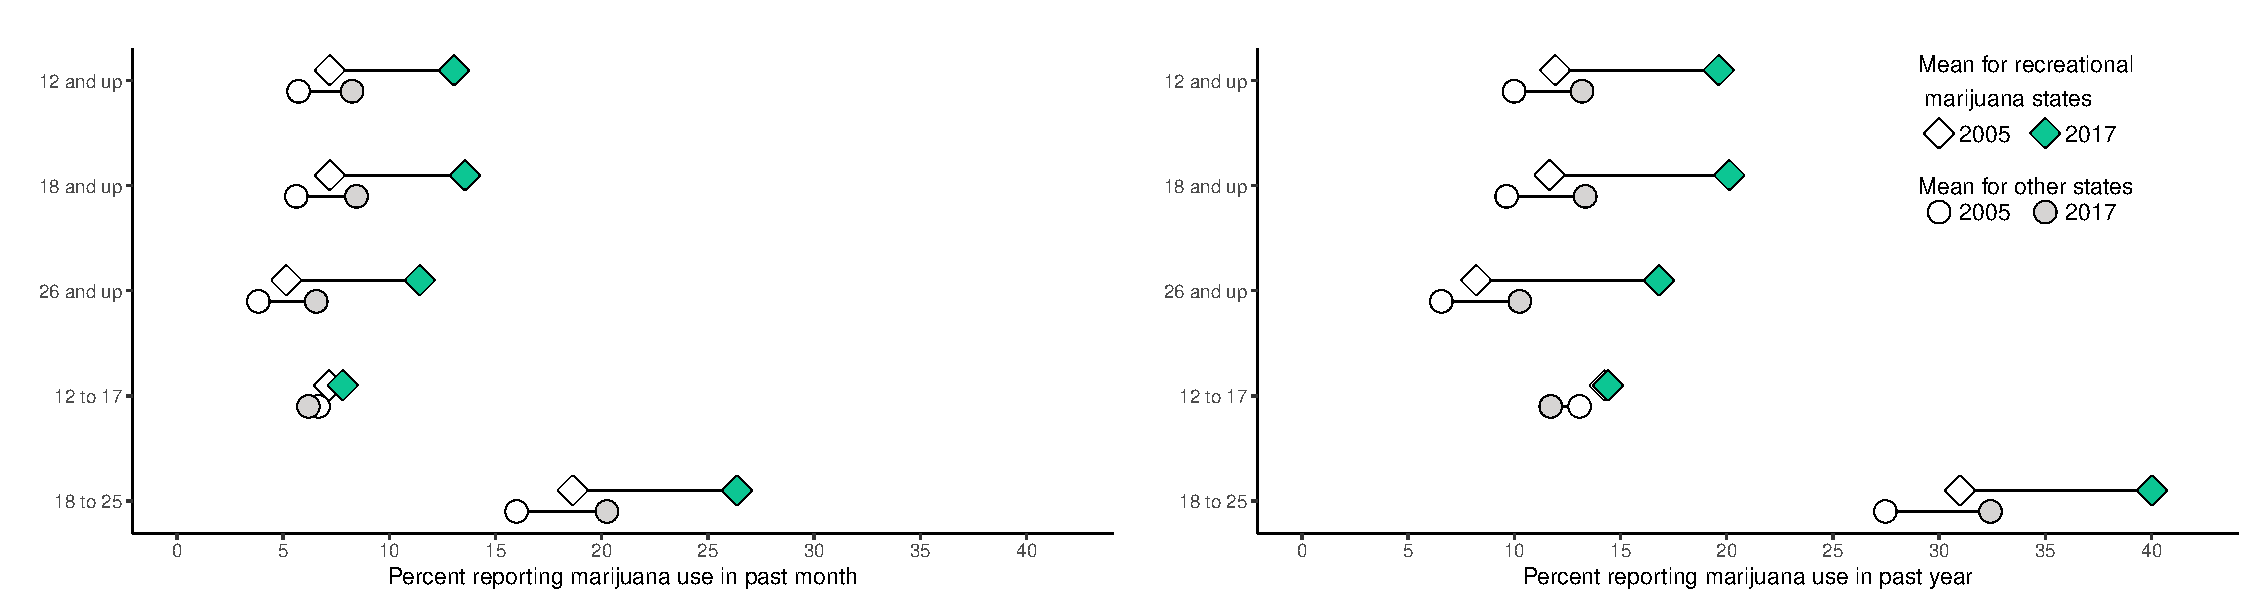
\includegraphics[width=\linewidth]{../output/plots/change-in-use-raw-data.pdf}
            \begin{justify}
            {\footnotesize
             \emph{Note:} 
            This figure presents the percent reporting marijuana use in the past-month (left panel) and past-year (right-panel) by age group. 
            %The top row displays the percent change from the 2005/2006 to 2016/2017. 
            The data are in these two-year averages due to the structure of the NSDUH SAE.   
            Data from 2005/2006 are displayed by the white shapes, while data from 2016/2016 are displayed by the shaded shapes.
            The green diamonds indicate data for recreational marijuana states, while the grey circles indicate all other states. 
            %The bottom row displays the difference in the percent change in use between recreational marijuana states and all other states by age group.  
                    \par}
                \end{justify}
        \end{minipage}
        \label{fig:change-in-mj-use-raw-data}
\end{figure}

    \end{landscape}

%------------------------------------------%
%     Figure AX - MJ Use over time
%------------------------------------------%
\begin{figure}[H]
    \caption{Comparing changes in marijuana use in different year}
    \begin{minipage}{.6\linewidth}
          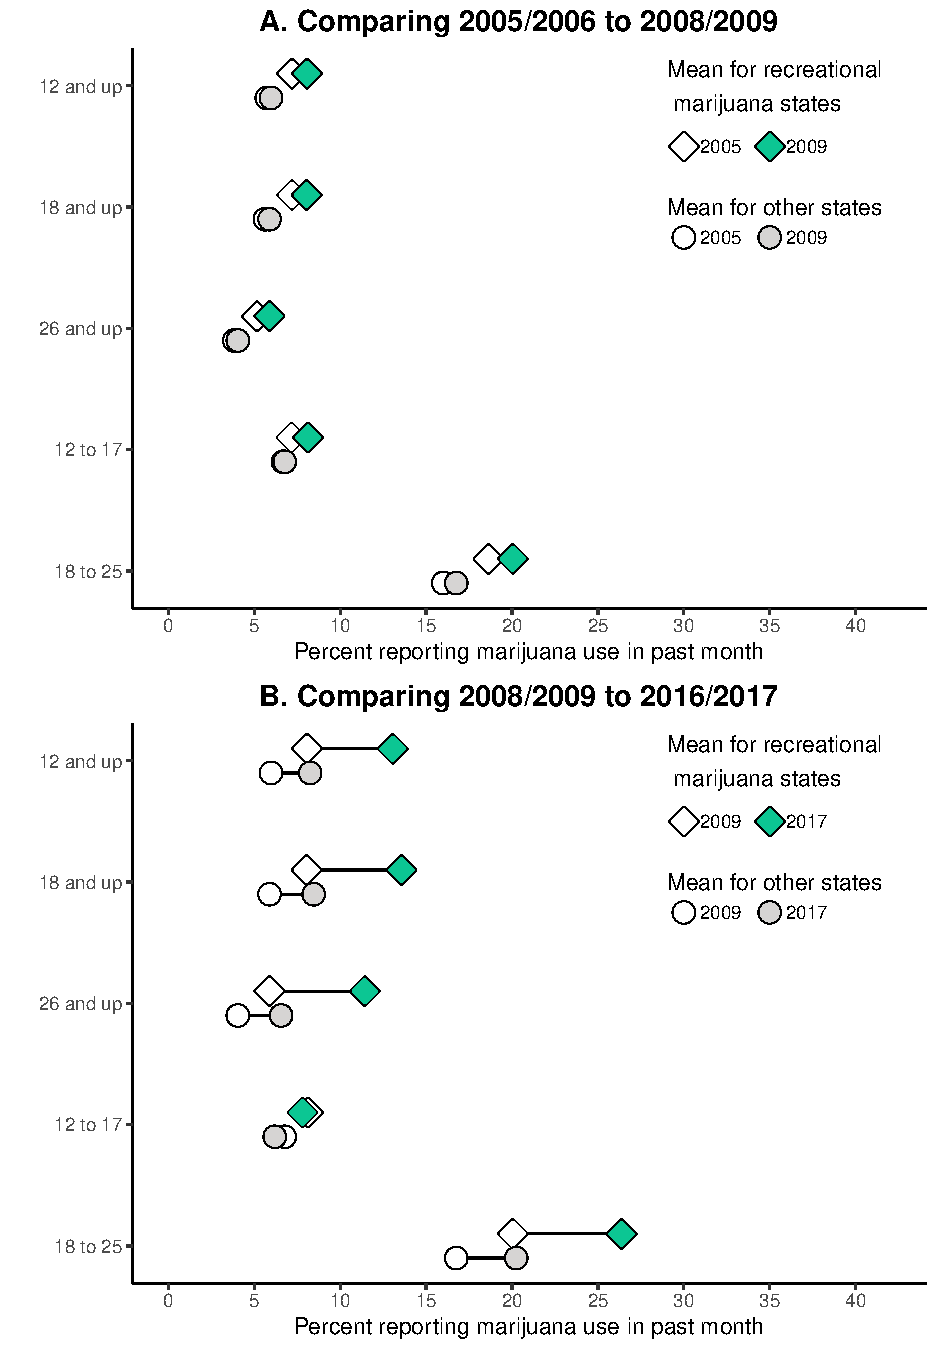
\includegraphics[width=\linewidth]{../output/plots/change-in-use-raw-data-additional-and-placebo.pdf}
                \begin{justify}
                    {\footnotesize
                        \emph{Note:} 
                        This figure presents the percent change in reported marijuana use in the past-month by age group and eventual-legality of marijuana. 
                        The top displays the change from the 2005/2006 to 2008/2009. 
                        The bottom displays the change from the 2008/2009 to 2016/2017. 
                        The data are in these two-year averages due to the structure of the NSDUH SAE.   
                        The green diamonds indicate changes for those in recreational marijuana states, while the grey circles indicate the same for all other states. 
                                \par}
                \end{justify}
    \end{minipage}
      \label{fig:change-in-mj-use-referee}
\end{figure}
%------------------------------------------%
%     Figure A
%------------------------------------------%
\begin{figure}[H]
\caption{States that adopted recreational marijuana laws saw larger than average increases in marijuana use from 2005 to 2017, showing each state}
  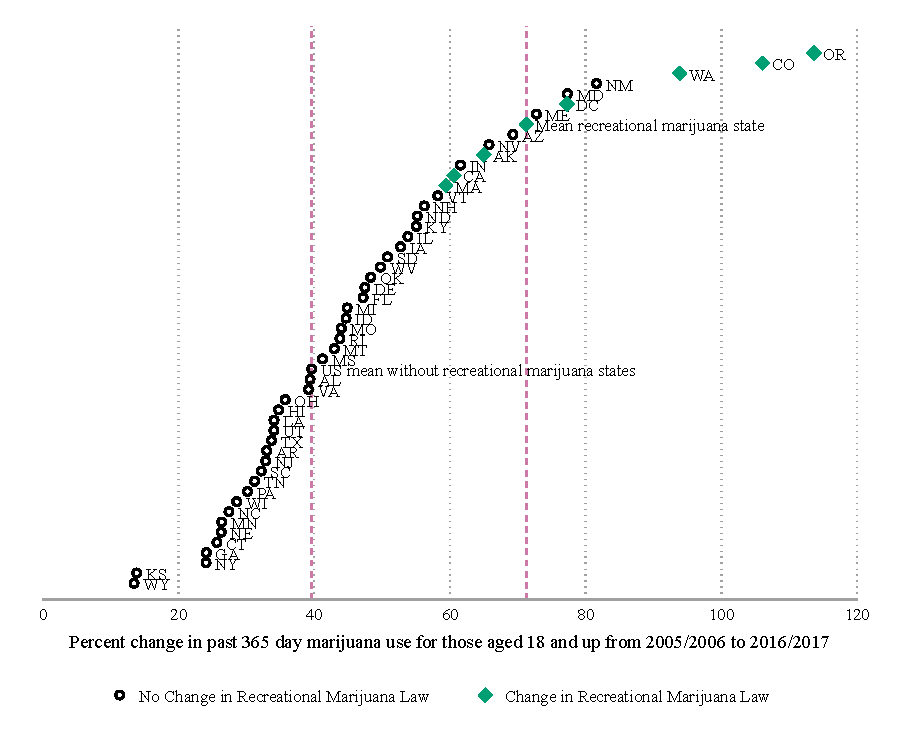
\includegraphics[width=\linewidth]{../output/plots/per_diff_mj_use_365_18.pdf}
   \label{fig:per_diff_mj_use_365_18}
\end{figure}
%------------------------------------------%
%     Figure AX - MJ Use over time
%------------------------------------------%
\begin{figure}[H]
    \caption{Marijuana use increased across all ages in recreational states compared to non-recreational states from 2005/2006 to 2016/2017}
    \begin{minipage}{\linewidth}
        \begin{minipage}{.49\linewidth}
          A. Aged 18+ \\
          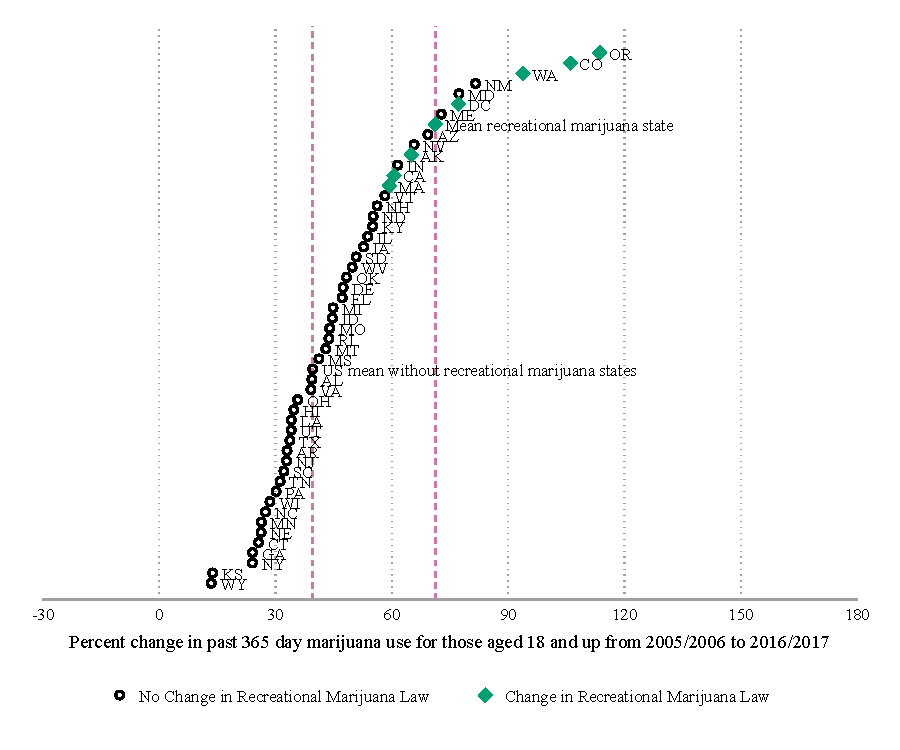
\includegraphics[width=\linewidth]{../output/plots/panel_per_diff_mj_use_365_18.pdf}
          C. Aged 12 to 17 \\
          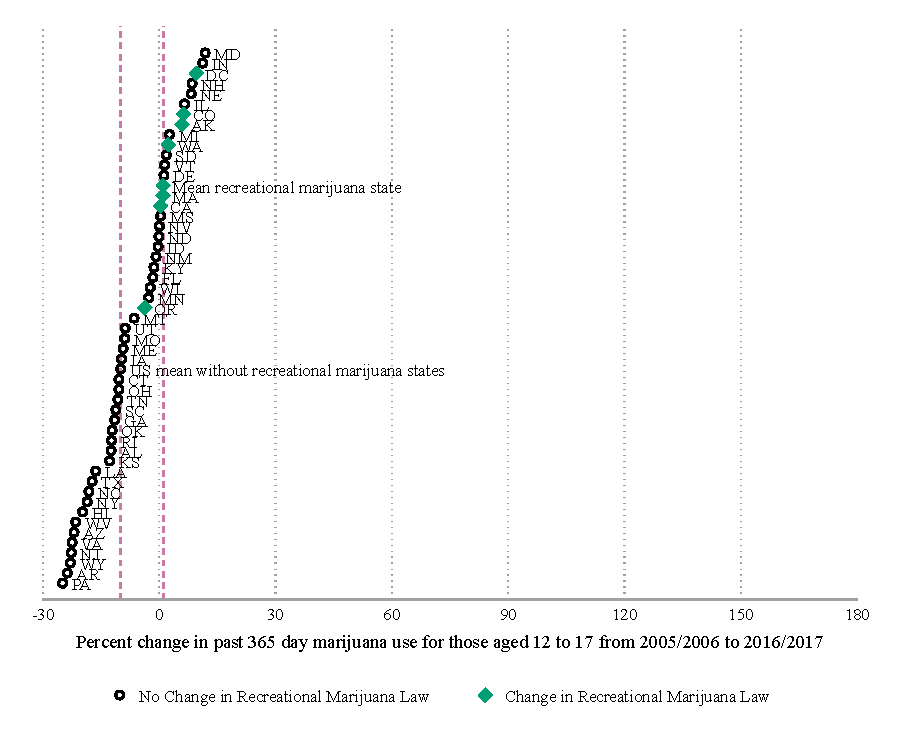
\includegraphics[width=\linewidth]{../output/plots/panel_per_diff_mj_use_365_12_17.pdf}
        \end{minipage}
        ~
        \begin{minipage}{.49\linewidth}
          B. Aged 26+\\
          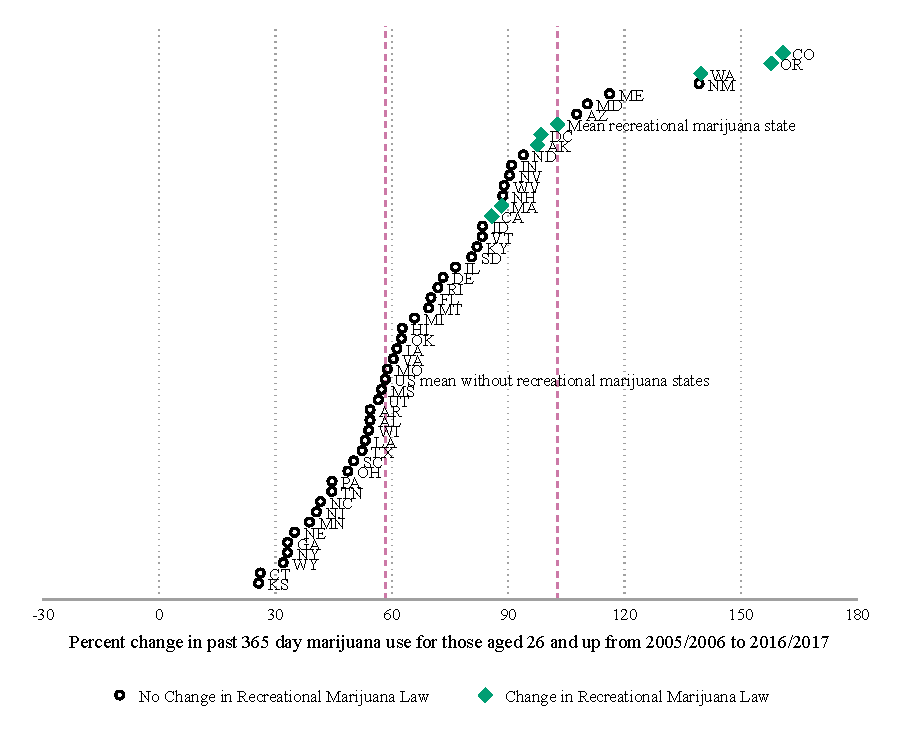
\includegraphics[width=\linewidth]{../output/plots/panel_per_diff_mj_use_365_26.pdf}
          D. Aged 18-25 \\
          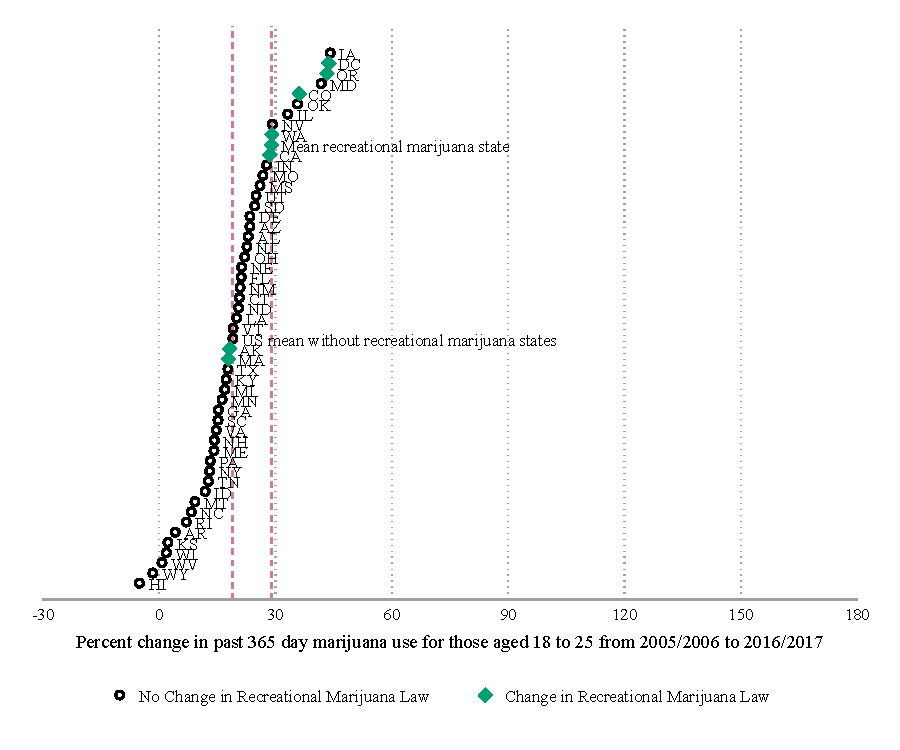
\includegraphics[width=\linewidth]{../output/plots/panel_per_diff_mj_use_365_18_25.pdf}
        \end{minipage}
    \end{minipage}
        \label{fig:mj-use-all-ages}
\end{figure}
   
%------------------------------------------%
%                Table A
%------------------------------------------%
% Summary statistics
\begin{table}[ht]\centering
    \begin{adjustbox}{width=\textwidth}
    \centering
      \begin{threeparttable}
        \caption{Summary statistics from non-substance use variables.}
        \estauto{../output/tables/summary_statistics_other_variables.tex}{9}{S[table-format=1.2,table-column-width=20mm]}
        \label{tab:summary_statistics_other}
      \end{threeparttable}
     \end{adjustbox}
\end{table}
\newpage
\FloatBarrier

%------------------------------------------%
%                Table A
%------------------------------------------%
% Recreational marijuana and marijuana use
\begin{table}[ht]\centering
  \begin{adjustbox}{width=.95\textwidth}
  \centering
    \begin{threeparttable}
      \caption{The impact of recreational marijuana on marijuana use by age group and frequency of use: without separating legalization and dispensary access.}
      \estauto{../output/tables/mj_table_no_rm_disp.tex}{6}{S[table-format=1.2,table-column-width=20mm]}
      \label{tab:mj_table_no_rm_disp}
     \Fignote{
         * p $<$ 0.1, ** p $<$ 0.05, *** p $<$ 0.01.
        The dependent variable is the natural log of the prevalence of drug use in state $s$ in period $t$ for a specified age group and type of drug. We use the model coefficients to compute $\% \Delta \approx 100\times \left[exp(\beta_1)-1\right]$, which is the percent change in the prevalence of drug use generated a given policy change.  We use a cluster robust variance matrix that allows for dependency at the state level to estimate standard errors for the coefficients, and we use the delta method to compute standard errors for the transformed coefficients. The standard errors are shown in parenthesis. The regressions adjust for unemployment rate, median income, \% white, and \% male.}
    \end{threeparttable}
   \end{adjustbox}
\end{table}
%------------------------------------------%
%                Table A
%------------------------------------------%

% Recreational marijuana and other substance use
  \begin{table}[ht]\centering
      \begin{adjustbox}{width=.90\textwidth}
      \centering
        \begin{threeparttable}
          \caption{The impact of recreational marijuana on substance use by age group and frequency of use:  without separating legalization and dispensary access.}
          \estauto{../output/tables/other_table_no_rm_disp.tex}{6}{S[table-format=1.2,table-column-width=20mm]}
          \label{tab:other_table_no_rm_disp}
         \Fignote{
            * p $<$ 0.1, ** p $<$ 0.05, *** p $<$ 0.01.
            The dependent variable is the natural log of the prevalence of drug use in state $s$ in period $t$ for a specified age group and type of drug. We use the model coefficients to compute $\% \Delta \approx 100\times \left[exp(\beta_1)-1\right]$, which is the percent change in the prevalence of drug use generated a given policy change.  We use a cluster robust variance matrix that allows for dependency at the state level to estimate standard errors for the coefficients, and we use the delta method to compute standard errors for the transformed coefficients. The standard errors are shown in parenthesis. The regressions adjust for unemployment rate, median income, \% white, and \% male.
          }  
        \end{threeparttable}
       \end{adjustbox}
    \end{table}
\FloatBarrier
 
%------------------------------------------%
%                Table A
%------------------------------------------%


\begin{figure}
    \caption{Event-study estimates of impact of recreational marijuana legalization, for early adopting states (CO and WA), by age group and frequency of marijuana use}
    \begin{minipage}{.9\linewidth}
        \begin{subfigure}[b]{0.32\columnwidth}
            \caption{\scriptsize{Marijuana use in past year}}
            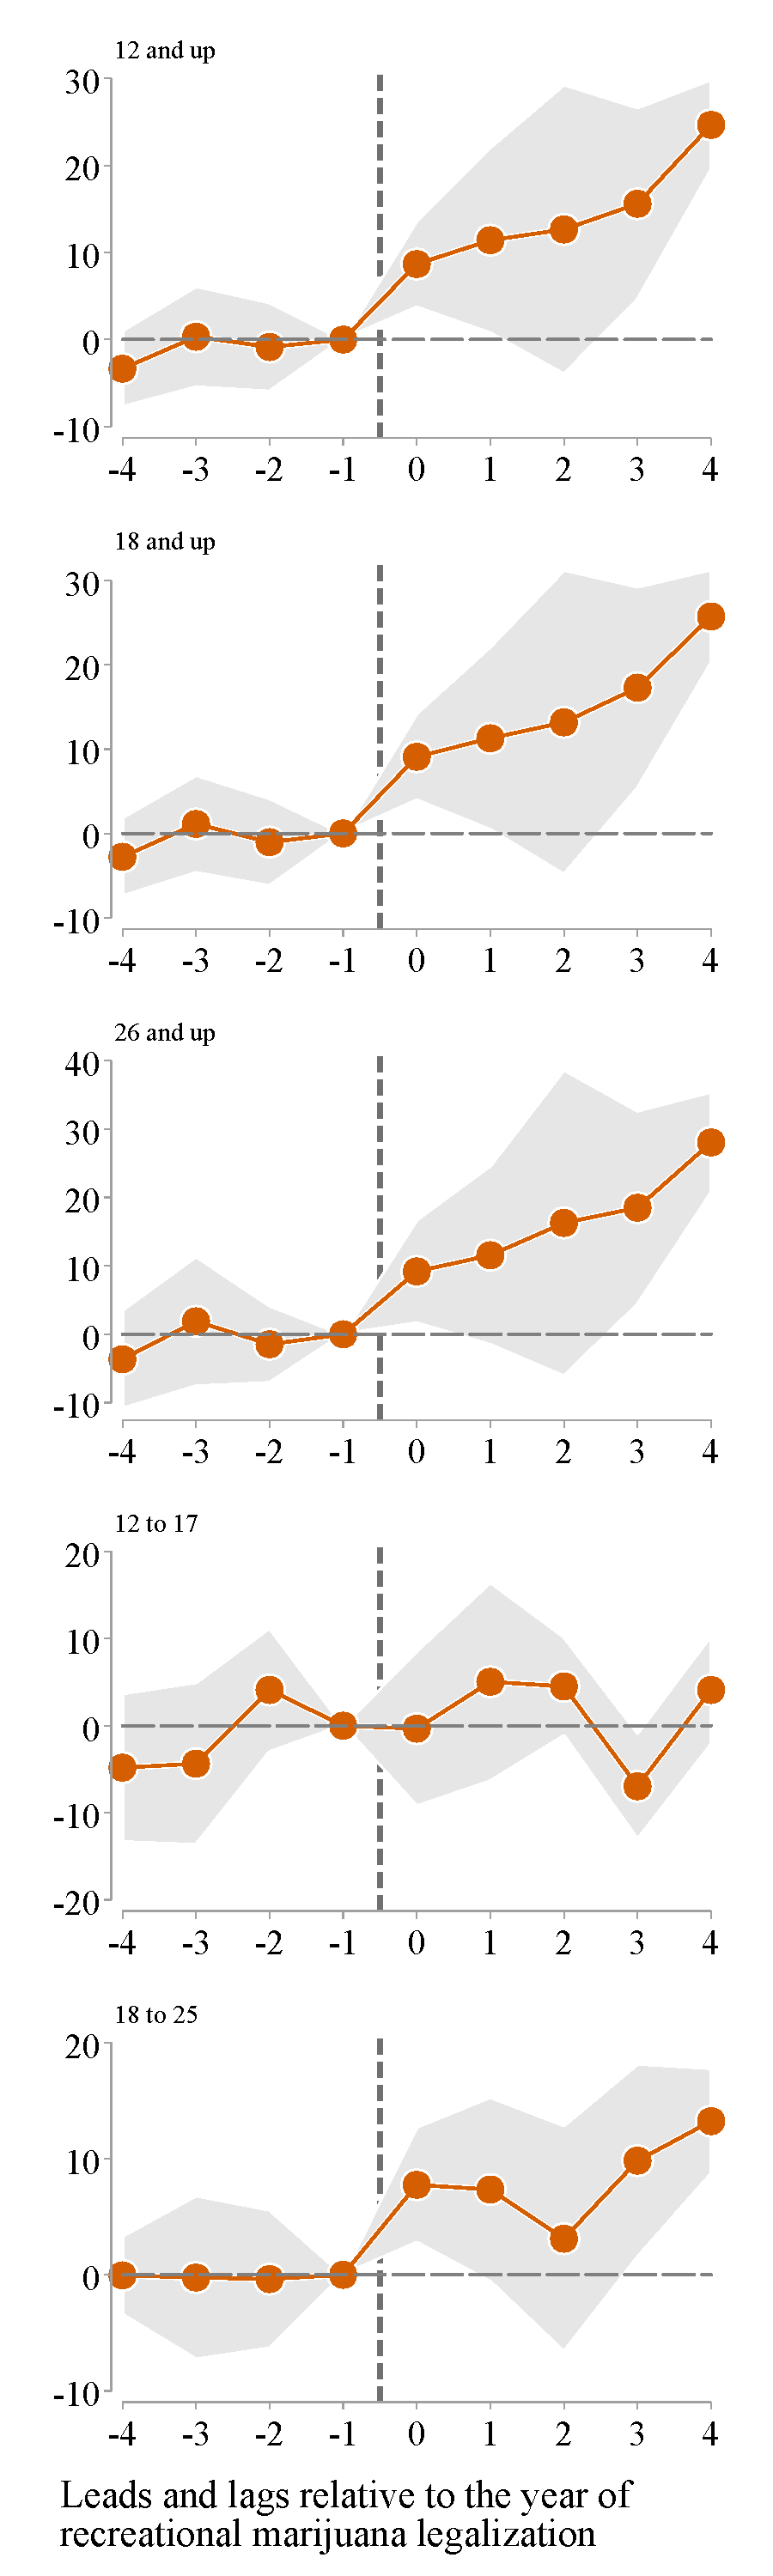
\includegraphics[width=\linewidth]{../output/plots/full-balanced-event-study-estimates-ln-mj_use_365.pdf}
        \end{subfigure}
            \hfill %%
        \begin{subfigure}[b]{0.32\columnwidth}
            \caption{\scriptsize{Marijuana use in past 30 days}}
            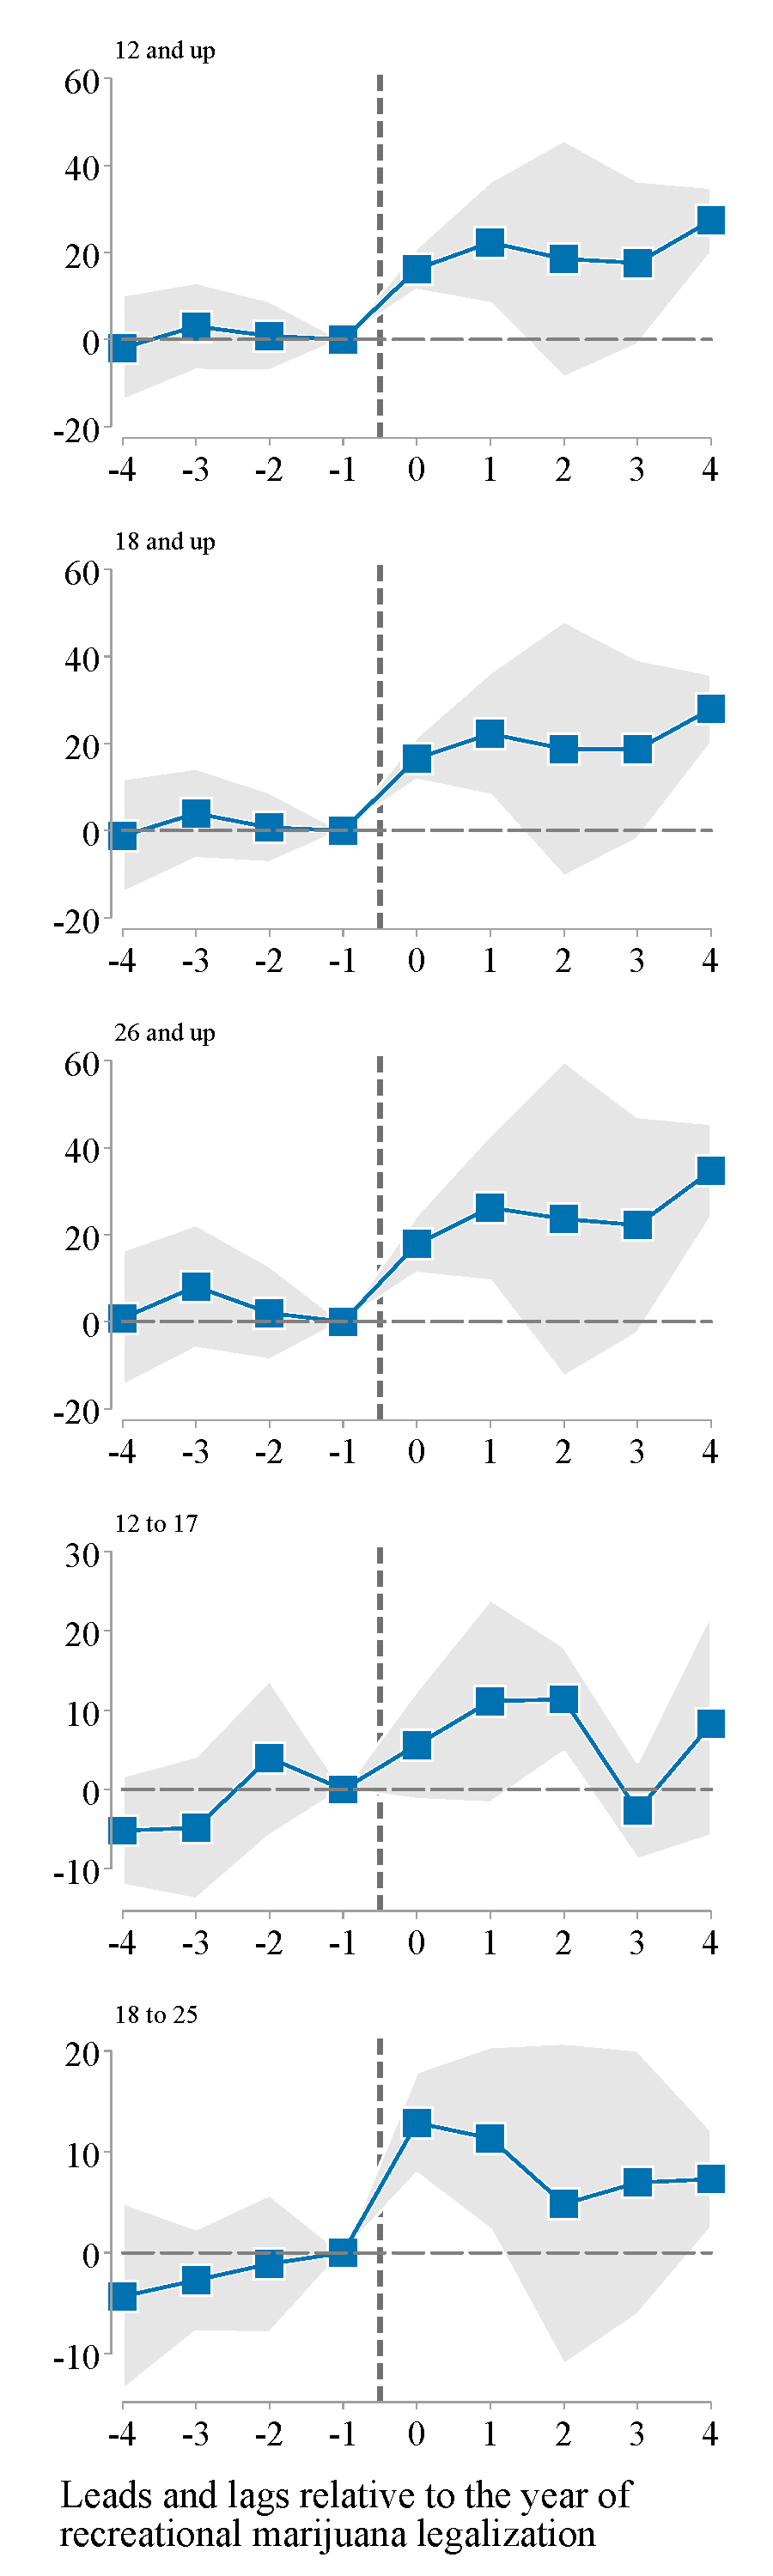
\includegraphics[width=\linewidth]{../output/plots/full-balanced-event-study-estimates-ln-mj_use_30.pdf}
        \end{subfigure}
            \hfill %%
        \begin{subfigure}[b]{0.32\columnwidth}
            \caption{\scriptsize{Marijuana initiates in past two years}}
            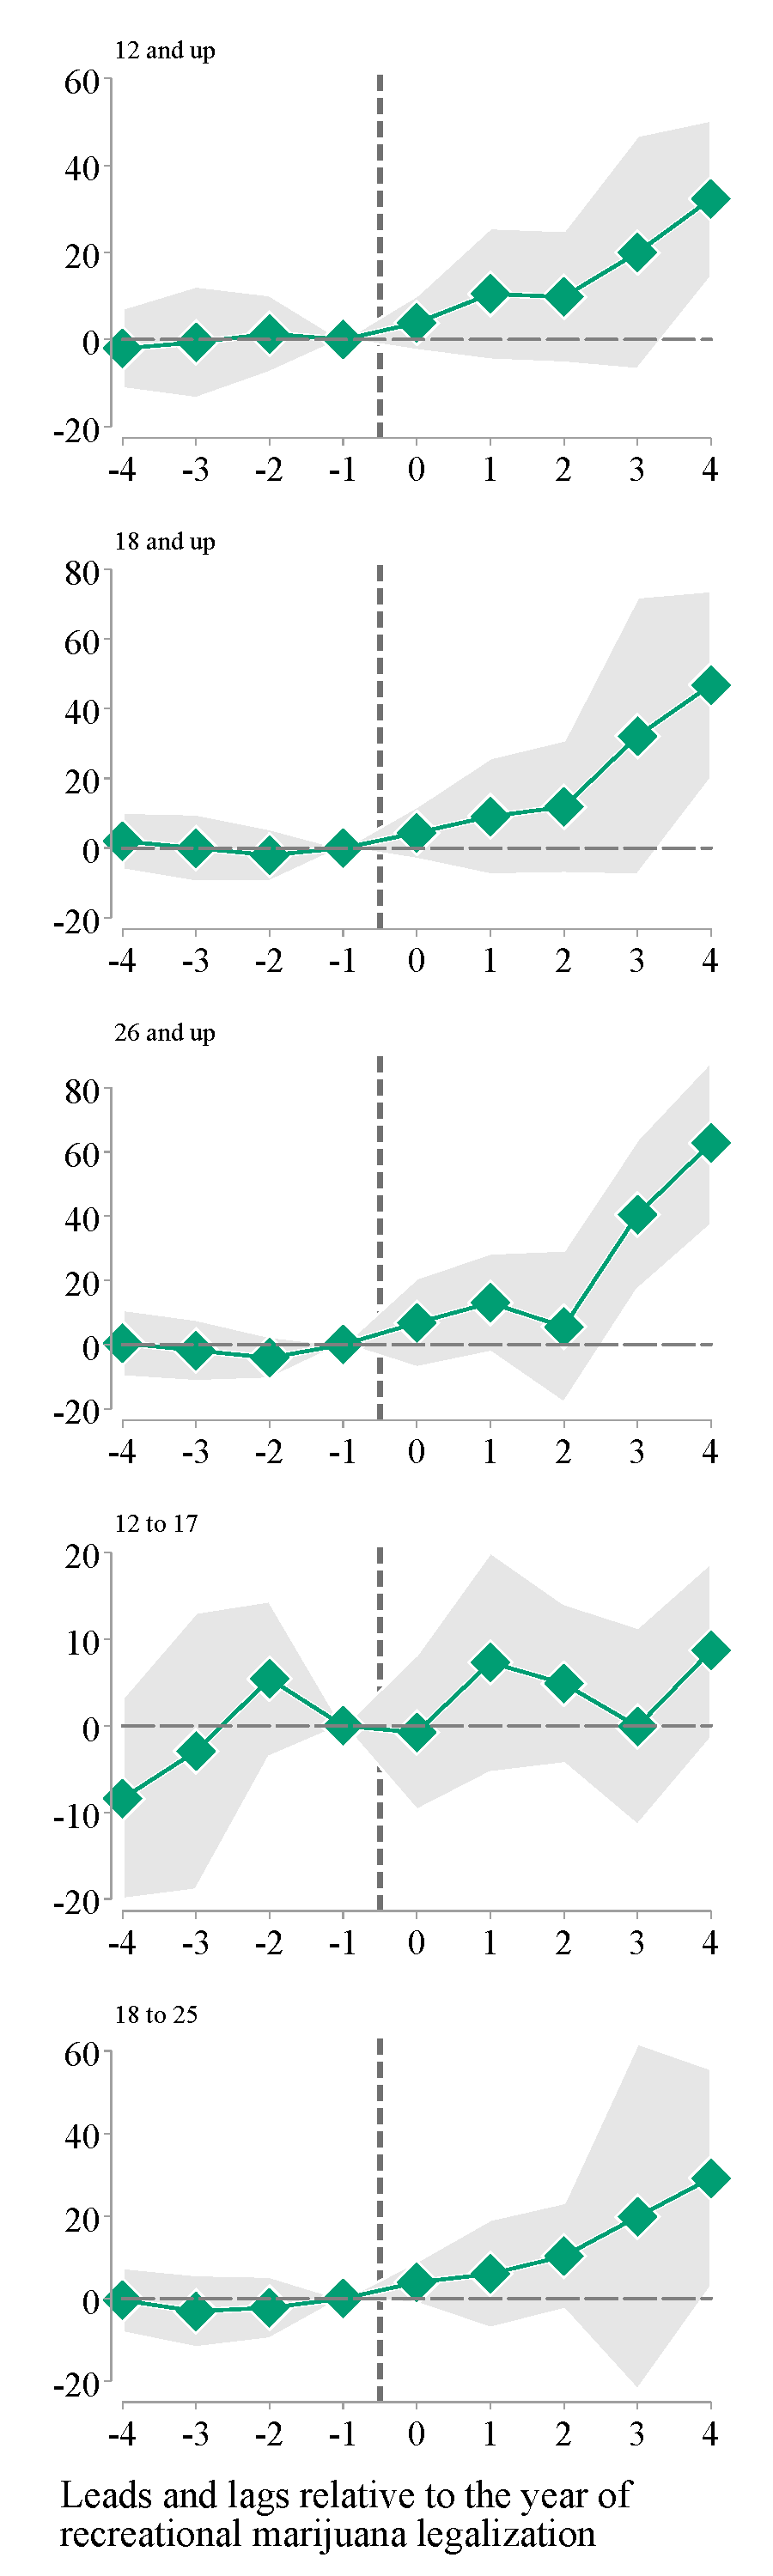
\includegraphics[width=\linewidth]{../output/plots/full-balanced-event-study-estimates-ln-mj_first_use.pdf}
        \end{subfigure}
        \begin{justify}
            {\footnotesize
            \emph{Note:} 
                Analyses in this figure include only states that did not adopt recreational marijuana in our sample time frame and the early adopting states of Colorado and Washington. This is to ensure a perfectly balanced composition of states contributing to the identification of each event-study point estimate. The dependent variable is the natural log of the prevalence of drug use in state $s$ in period $t$ for a specified age group and type of drug. We use the model coefficients to compute $\% \Delta \approx 100\times \left[exp(\beta_1)-1\right]$, which is the percent change in the prevalence of drug use generated a given policy change.  We use a cluster robust variance matrix that allows for dependency at the state level to estimate standard errors for the coefficients, and we use the delta method to compute standard errors for the transformed coefficients and associated 95\% confidence intervals, which are reported by the shaded area. The standard error refers to the standard error of the combined effect. The regressions adjust for unemployment rate, median income, \% white, and \% male. 
            \par}
        \end{justify}
    \end{minipage}
    \label{fig:event-study-early-adopters}
\end{figure}

\end{document}